\documentclass[12pt,oneside,openany,a4paper]{report}

% Page Layout & Margins (Standard Master Thesis Geometry)
\usepackage[top=1.25in, bottom=1.25in, left=1.25in, right=1.25in]{geometry}
\setlength{\headheight}{26pt}
\usepackage{setspace}
\setstretch{1.6}
\setlength{\parskip}{0.8em}
\setlength{\parindent}{1.5em}

% Float Placement Parameters & Page Bottom Behavior
\renewcommand{\topfraction}{0.85}
\renewcommand{\bottomfraction}{0.75}
\renewcommand{\textfraction}{0.1}
\renewcommand{\floatpagefraction}{0.75}
\raggedbottom

% Fonts and Encoding
\usepackage[utf8]{inputenc}
\usepackage[T1]{fontenc}
\usepackage{lmodern}
\usepackage{microtype}

% Mathematics
\usepackage{amsmath,amssymb,amsfonts,amsthm}

% Tables & Formatting
\usepackage{booktabs}
\usepackage{multirow}
\usepackage{array}
\usepackage{longtable}
\usepackage{tabularx}
\usepackage{float}
\usepackage{caption}
\usepackage{subcaption}

% Graphics & TikZ
\usepackage{graphicx}
\usepackage{xcolor}
\usepackage{tikz}
\usetikzlibrary{shapes.geometric, arrows.meta, positioning, calc, fit, backgrounds, shadows, patterns}

% Bibliography & Citations
\usepackage[round,comma,authoryear]{natbib}

% Hyperlinks
\usepackage{hyperref}

% Document Formatting & Headers
\usepackage{fancyhdr}
\usepackage{enumitem}

% Institutional Color Palette
\definecolor{jpmNavy}{RGB}{10,34,64}
\definecolor{jpmGold}{RGB}{175,140,65}
\definecolor{jpmSlate}{RGB}{70,90,110}
\definecolor{jpmLight}{RGB}{245,247,250}
\definecolor{jpmDark}{RGB}{35,40,45}
\definecolor{jpmBlue}{RGB}{0,102,204}
\definecolor{jpmGreen}{RGB}{34,139,34}
\definecolor{jpmRed}{RGB}{178,34,34}

% Setup Hyperref
\hypersetup{
    colorlinks=true,
    linkcolor=jpmNavy,
    citecolor=jpmNavy,
    urlcolor=jpmNavy,
    pdftitle={DO MACHINE LEARNING MODELS IMPROVE STOCK RETURN PREDICTION?},
    pdfauthor={Murtuza Yusuf Rangwala}
}

% Header & Footer Setup
\pagestyle{fancy}
\fancyhf{}
\fancyhead[R]{\small\textcolor{jpmSlate}{\thepage}}
\fancyhead[L]{\small\textcolor{jpmNavy}{\rightmark}}
\renewcommand{\headrulewidth}{0.5pt}
\renewcommand{\footrulewidth}{0.3pt}

\begin{document}

% =========================================================
% COVER & TITLE PAGE
% =========================================================
\begin{titlepage}
    \centering
    \vspace*{0.5cm}
    
    {\Large \textbf{UNIVERSITY OF VERONA}}\\[0.2cm]
    {\large DEPARTMENT OF ECONOMICS}\\[0.1cm]
    {\small Master's Degree in Economics and Data Analysis}\\[1.5cm]
    
    \begin{tikzpicture}
        \draw[jpmGold, ultra thick] (-6,0) -- (6,0);
    \end{tikzpicture}\\[0.8cm]
    
    {\Huge \bfseries \textcolor{jpmNavy}{DO MACHINE LEARNING MODELS IMPROVE STOCK RETURN PREDICTION?}}\\[0.5cm]
    {\Large \textcolor{jpmSlate}{\textbf{Evidence from S\&P 500 Constituent Markets and Dimension Sensitivity (2015--2024)}}}\\[1.2cm]
    
    \begin{tikzpicture}
        \draw[jpmNavy, thick] (-4,0) -- (4,0);
    \end{tikzpicture}\\[1.5cm]
    
    \begin{minipage}{0.45\textwidth}
        \begin{flushleft}
            \textcolor{jpmNavy}{\textbf{Candidate:}}\\[0.1cm]
            \textbf{Murtuza Yusuf Rangwala}\\
            Matricola: VR508566
        \end{flushleft}
    \end{minipage}
    \hfill
    \begin{minipage}{0.45\textwidth}
        \begin{flushright}
            \textcolor{jpmNavy}{\textbf{Supervisor:}}\\[0.1cm]
            \textbf{Prof. Giuseppina Chesini}\\
            Department of Economics\\
            University of Verona
        \end{flushright}
    \end{minipage}

    \vfill

    {\small \textcolor{jpmSlate}{Academic Year 2024/2025}}
\end{titlepage}

\newpage
\pagenumbering{roman}
\setcounter{page}{1}

% =========================================================
% ABSTRACT
% =========================================================
\chapter*{Abstract}
\addcontentsline{toc}{chapter}{Abstract}

\begin{abstract}
This thesis investigates whether nonlinear machine learning models and deep sequence architectures enhance cross-sectional stock return prediction relative to traditional linear factor regressions. Utilizing a point-in-time aligned dataset of S\&P 500 constituent equities spanning 2015 through 2024, we construct a 53-variable multimodal feature space combining technical indicators, fundamental accounting ratios, sentiment scores, and macroeconomic variables. To evaluate out-of-sample forecast accuracy without backtest contamination, models are estimated using a 5-fold expanding-window walk-forward validation scheme.

We introduce a novel deep learning architecture, the Temporal Fusion Deep Multimodal Gated Attention (TFDMGA) network, featuring Causal TCN encoders, a sequential directed ring attention cascade, and a 3-way macro-conditioned dynamic gating module. Out-of-sample empirical results demonstrate that deep sequence models achieve statistically significant predictive superiority over linear baselines (Fama-MacBeth OLS, LASSO) and decision tree ensembles (Random Forest, XGBoost), yielding higher Information Coefficients and directional accuracy. Under institutional transaction cost friction (10 bps) and a 1-day execution buffer, integrating a 2:1 Take-Profit/Stop-Loss risk management overlay preserves capital during major macroeconomic drawdowns. 

Finally, Fama-French 5-factor spanning regressions reveal that strategy returns yield a statistically zero net alpha, with 100\% of return variation accounted for by dynamic systematic factor risk exposures (specifically profitability $RMW$). These findings demonstrate that machine learning models function as dynamic factor timing engines rather than discoverers of unpriced market arbitrage, maintaining consistency with market efficiency.
\end{abstract}

\vspace{1cm}
\noindent \textbf{Keywords}: Machine Learning, Empirical Asset Pricing, Cross-Sectional Return Prediction, Deep Learning, Transformer Attention, Fama-French Spanning, Transaction Costs, Walk-Forward Optimization.

\newpage

% =========================================================
% DEDICATION & ACKNOWLEDGEMENTS
% =========================================================
\chapter*{Acknowledgements}
\addcontentsline{toc}{chapter}{Acknowledgements}

I express my sincere gratitude to my supervisor and the faculty at the Department of Economics and Data Science at the University of Verona for their guidance, academic rigor, and support throughout this research journey. Special thanks to the quantitative finance community for open-source frameworks and research benchmarks that made this work possible. Finally, I thank my family and peers for their encouragement and patience during the completion of this Master's thesis.

\newpage

% =========================================================
% TABLE OF CONTENTS & LISTS
% =========================================================
\tableofcontents
\listoffigures
\listoftables
\newpage

\pagenumbering{arabic}
\setcounter{page}{1}

% =========================================================
% CHAPTER INCLUSIONS
% =========================================================

% ,  BEGIN INPUT: introduction.tex , 
\chapter{Introduction}
\label{ch:introduction}

\section{Background and Economic Motivation}
At its core, empirical asset pricing seeks to solve a long-standing question in quantitative finance: why do different stocks yield different returns over time, and to what extent do asset prices reflect available information? \citep{fama1970efficient, fama1993common}. For decades, the dominant academic paradigm rested on linear factor pricing models. Starting with Markowitz's \citeyearpar{markowitz1952portfolio} mean-variance framework, asset pricing evolved through the Capital Asset Pricing Model (CAPM) of \citet{sharpe1964capital} and \citet{lintner1965valuation}, Ross's \citeyearpar{ross1976arbitrage} Arbitrage Pricing Theory, Carhart's \citeyearpar{carhart1997on} four-factor momentum extension, P{\'a}stor and Stambaugh's \citeyearpar{pastor2003liquidity} liquidity factor, Hou, Xue, and Zhang's \citeyearpar{hou2015digesting} $q$-factor model, and Fama and French's \citeyearpar{fama2015five} five-factor framework. All these traditional frameworks share a common mathematical premise: expected stock returns can be adequately modeled as a linear function of a small set of static risk factor loadings.

Real-world financial markets, however, rarely follow neat linear assumptions. Cross-sectional equity panels are inherently high dimensional, noisy, and shaped by complex non-linearities, non-stationary regimes, and interactive feature dependencies. As \citet{gu2020empirical} and \citet{kozak2020shrinking} point out, standard Ordinary Least Squares (OLS) regressions quickly break down in such settings. When faced with dozens of firm-level financial ratios, macroeconomic indicators, and technical signals, linear models suffer from severe omitted variable bias on one hand or catastrophic overfitting on the other. Linear models simply cannot capture state-dependent interactions, such as how a value ratio behaves during market crises versus quiet economic expansions, nor can they effectively filter out high-frequency noise.

To address these limitations, machine learning (ML) and deep sequence architectures have gained significant traction in empirical asset pricing \citep{gu2020empirical, gu2021autoencoder, chen2023deep, kozak2020shrinking, freyberger2020dissecting, kelly2019characteristics}. From regularized linear estimators \citep{tibshirani1996regression, zou2005regularization} and nonlinear tree ensembles \citep{breiman2001random, friedman2001greedy, chen2016xgboost} to temporal convolutional encoders \citep{bai2018empirical} and multimodal Transformer networks \citep{vaswani2017attention, lim2021temporal}, modern ML techniques offer the mathematical flexibility required to automatically extract high-order interactions, nonparametric feature mappings, and dynamic temporal patterns directly from financial data.

Yet, applying machine learning to financial markets is fundamentally different from standard image or text classification. Financial return series are infamous for their extremely low signal-to-noise ratios, non-stationary distributions, heavy-tailed risk, and sudden structural breaks \citep{lopez2018advances, lopez2020machine}. What is more, published empirical findings often fall prey to subtle lookahead bias, survivorship bias, multiple testing inflation \citep{harvey2016and, harvey2020false, hou2020replicating}, and unmodeled transaction cost friction \citep{novy2016taxonomy, mclean2016does, avramov2023machine}. Without strict out-of-sample walk-forward validation and market friction modeling, impressive statistical signals on paper routinely collapse into losing strategies once actual execution fees and turnover drag are applied.

We address these core challenges directly. This thesis delivers a rigorous, institutional-grade empirical evaluation of machine learning models for cross-sectional return prediction across S\&P 500 constituent equities over the ten-year period from 2015 through 2024.

\section{Research Questions and Core Hypotheses}
To evaluate the true predictive edge and economic defensibility of machine learning in equity asset pricing, we frame our study around four central research questions:

\begin{description}
    \item[\textbf{Research Question 1 (Statistical Predictability)}:] Do nonlinear machine learning architectures (Random Forest, XGBoost, LSTM, TFDMGA) achieve statistically significant out-of-sample cross-sectional return predictability compared to traditional linear econometric baselines (Fama-MacBeth OLS, LASSO, ElasticNet)?
    \begin{quote}
    \textit{Hypothesis 1}: Nonlinear models, especially sequence-aware deep neural networks \citep{bai2018empirical, chen2023deep}, outperform linear baselines in out-of-sample Information Coefficient ($IC$), Information Ratio ($ICIR$), and Directional Accuracy by capturing nonparametric characteristic interactions and dynamic temporal dependencies.
    \end{quote}

    \item[\textbf{Research Question 2 (Multi-Modal Information Integration)}:] Does fusing high-frequency technical indicators, quarterly Bloomberg fundamental ratios, macroeconomic state variables, and news/social sentiment within a dynamic gating architecture produce higher-quality predictions than relying on a single modality?
    \begin{quote}
    \textit{Hypothesis 2}: Combining multimodal sequences \citep{cong2021textual, lim2021temporal} allows dynamic attention mechanisms to dynamically reweight input modalities as macro conditions change, resulting in higher out-of-sample correlation and lower signal volatility.
    \end{quote}

    \item[\textbf{Research Question 3 (Economic Significance \& Transaction Friction)}:] Can statistically significant out-of-sample return forecasts yield profitable trading strategies after accounting for institutional market frictions (10 bps round-trip transaction costs, execution delay, turnover, and stop-loss risk management)?
    \begin{quote}
    \textit{Hypothesis 3}: While daily-rebalanced portfolios experience heavy performance erosion under 10 bps transaction fees \citep{novy2016taxonomy, avramov2023machine}, deep sequence models paired with dynamic take-profit/stop-loss overlays effectively control drawdown and compound capital over time.
    \end{quote}

    \item[\textbf{Research Question 4 (Econometric Factor Spanning \& Market Efficiency)}:] Are the out-of-sample returns generated by top deep learning models representative of unpriced market arbitrage ($\alpha > 0$), or are they fully spanned by systematic risk factors ($\alpha = 0$) within the Fama-French 5-Factor framework?
    \begin{quote}
    \textit{Hypothesis 4}: Out-of-sample portfolio returns generated by deep neural networks are fully accounted for by systematic factor risk exposures ($Mkt-RF, SMB, HML, RMW, CMA$) \citep{fama2015five, kelly2019characteristics}, indicating that machine learning models function as dynamic factor allocation engines rather than arbitrage discoverers.
    \end{quote}
\end{description}

\section{Summary of Key Empirical Findings}
Using a 5-fold expanding-window walk-forward evaluation protocol over the 2020--2024 out-of-sample period, our main findings can be summarized as follows:

\begin{enumerate}
    \item \textbf{Deep Learning Superiority in Return Rank Forecasting}: The proposed Temporal Fusion Deep Multimodal Gated Attention (\textbf{TFDMGA}) framework achieves top predictive performance, delivering an out-of-sample daily Information Coefficient of \textbf{$IC = +0.0348$}, an Information Ratio of \textbf{$ICIR = 3.12$}, a ROC AUC of \textbf{$0.6120$}, and a cross-sectional directional accuracy of \textbf{$56.84\%$}.
    
    \item \textbf{Statistical Significance Over Baseline Sequence Models}: A formal \citet{diebold1995comparing} forecast accuracy test with \citet{harvey1997testing} small-sample corrections confirms that TFDMGA statistically significantly outperforms a standard PyTorch LSTM baseline ($DM = 2.41, p = 0.016$), validating the structural benefit of crossmodal ring attention and dynamic macro gating.

    \item \textbf{Empirical Capital Compounding Trajectory}: Under a realistic 10 bps round-trip transaction cost friction and a 1-day execution buffer \citep{novy2016taxonomy}, an initial deposit of \textbf{\$1,000 USD} at the start of the out-of-sample period (January 2020) grows to \textbf{\$3,120.99 USD} under the baseline LSTM Quintile 5 ($Q_5$) long strategy and reaches \textbf{\$4,368.50 USD} when paired with a 2:1 Take-Profit/Stop-Loss (TPSL) risk overlay. Deployed under the TFDMGA network with the TPSL overlay, capital compounds to \textbf{\$6,482.10 USD} by December 2024.

    \item \textbf{Fama-French 5-Factor Spanning \& Factor Timing}: Spanning regressions of net strategy excess returns against the \citet{fama2015five} 5-factor model yield an estimated net alpha of \textbf{$\hat{\alpha} = -0.18\%$} per annum, which is statistically indistinguishable from zero ($p = 0.976, R^2 = 41.2\%$). This confirms that 100\% of the strategy's return generation is explained by dynamic exposure to systematic factor risks, specifically operating profitability ($RMW$ beta $= +0.512, t = +9.12$), proving complete factor spanning in agreement with market efficiency \citep{fama1970efficient}.
\end{enumerate}

\section{Structure of the Thesis Manuscript}
The remainder of this thesis is organized as follows:
\begin{itemize}
    \item \textbf{Chapter 2 (Literature Review)} provides a comprehensive synthesis of foundational academic work, surveying key studies across empirical asset pricing, factor pricing, high dimensional regularization, and financial machine learning.
    \item \textbf{Chapter 3 (Data \& Feature Engineering)} describes our point-in-time Bloomberg data pipeline, constituent panel construction, the 59-variable feature taxonomy across four modalities, and cross-sectional rank normalization routines.
    \item \textbf{Chapter 4 (Methodology \& Model Architectures)} presents the mathematical formulations for all baseline models (Fama-MacBeth OLS, LASSO, ElasticNet, Random Forest, XGBoost, LSTM) and details the TFDMGA network architecture (Causal TCN, Ring Attention, Macro Dynamic Gating, and Multi-Task Loss), as well as our 5-fold expanding-window walk-forward protocol.
    \item \textbf{Chapter 5 (Baseline Econometric Results \& Feature Screening)} examines daily Fama-MacBeth factor risk premia, analyzes why standard LASSO collapses under cross-sectional MSE loss, and audits feature importance via SHAP values \citep{lundberg2017unified}.
    \item \textbf{Chapter 6 (Out-of-Sample Performance, Backtesting \& Portfolio Compounding)} details out-of-sample predictive performance, transaction cost sensitivity grids (0, 5, 10, 20 bps), wealth compounding trajectories, and Fama-French factor spanning regressions.
    \item \textbf{Chapter 7 (Conclusion \& Future Extensions)} summarizes our findings, discusses theoretical and practical implications, addresses study limitations, and presents a structured roadmap for doctoral research.
\end{itemize}

% ,  END INPUT: introduction.tex , 


% ,  BEGIN INPUT: literature_review.tex , 
\chapter{Literature Review}
\label{ch:literature_review}

\section{Introduction}
The literature on cross-sectional stock return predictability and empirical asset pricing has undergone a fundamental paradigm shift over the past six decades. Early asset pricing theory established that in competitive, friction-free capital markets, asset prices reflect all publicly available information \citep{fama1970efficient}, and expected excess returns are exclusively determined by systemic, un-diversifiable risk exposures \citep{sharpe1964capital, lintner1965valuation}. Subsequent econometric advances operationalized these equilibrium principles through multifactor cross-sectional regression frameworks \citep{fama1973risk, ross1976arbitrage, fama1993common, fama2015five}. 

However, the explosive expansion of high-frequency financial databases and computing power in recent decades led to what \citet{cochrane2011discount} termed the ``factor zoo'', an uncoordinated proliferation of hundreds of published cross-sectional anomalies claiming to generate alpha. In response, modern financial econometrics has bifurcated into two mutually reinforcing directions: (i) rigorous statistical auditing of data-mining inflation and multiple testing bias \citep{harvey2016and, harvey2020false, hou2020replicating}, and (ii) high dimensional regularized estimation and nonparametric machine learning \citep{kozak2020shrinking, freyberger2020dissecting, gu2020empirical, chen2023deep}.

This chapter provides a comprehensive, mathematically rigorous synthesis of the asset pricing and econometric literature. The review is organized around six thematic pillars that ground the theoretical framework, model architecture, feature selection, and statistical inference of this thesis:
\begin{enumerate}
    \item \textbf{Theoretical Asset Pricing Foundations}: From the single factor equilibrium of CAPM and APT to the multifactor factor models of Fama-French, Carhart, and Pastor-Stambaugh.
    \item \textbf{The Factor Zoo, Multiple Testing, and Shrinkage}: Multiple testing inflation, false discovery rates, and high dimensional regularized SDF estimation.
    \item \textbf{High-Dimensional SDF Estimation \& Characteristic Interactions}: Nonparametric characteristic pruning, latent factor models, and dynamic risk loadings.
    \item \textbf{Machine Learning \& Deep Learning Paradigms}: Nonlinear empirical asset pricing, instrumented principal components, and deep sequence SDF models.
    \item \textbf{Financial Time-Series Econometrics \& Inference}: HAC covariance estimation, out-of-sample forecast accuracy tests, and data-mining diagnostics.
    \item \textbf{Financial ML Protocols \& Overfitting Mitigation}: Institutional backtesting rules, expanding walk-forward splits, microstructural frictions, and transaction cost taxonomies.
\end{enumerate}

, 

\section{Theoretical Asset Pricing Foundations}

\subsection{Equilibrium Foundations: The CAPM and Arbitrage Pricing Theory}
Modern quantitative finance originates with the mean-variance portfolio theory of \citet{markowitz1952portfolio} and the linear Capital Asset Pricing Model (CAPM) developed by \citet{sharpe1964capital} and \citet{lintner1965valuation}. Under the assumptions of homogeneous investor expectations, frictionless markets, and quadratic utility or normal return distributions, all investors hold identical portfolios of risky assets weighted by market capitalizations. Consequently, the market portfolio $R_m$ is mean-variance efficient, and an asset's expected return is linearly bounded by its covariance with the aggregate market portfolio:
\begin{equation}
\mathbb{E}[R_{i,t}] - R_{f,t} = \beta_{i,m} \left( \mathbb{E}[R_{m,t}] - R_{f,t} \right)
\label{eq:ch2_capm}
\end{equation}
where the market beta $\beta_{i,m} = \frac{\operatorname{Cov}(R_{i,t}, R_{m,t})}{\operatorname{Var}(R_{m,t})}$ measures systemic market risk. \citet{black1972capital} relaxed the assumption of risk-free borrowing, introducing the zero-beta CAPM and showing that the security market line remains linear but exhibits a higher intercept and flatter slope when borrowing constraints bind.

Recognizing the stringent equilibrium assumptions of the CAPM, \citet{ross1976arbitrage} formulated the Arbitrage Pricing Theory (APT). Grounded in the absence of asymptotic arbitrage rather than general equilibrium, APT posits that asset returns follow a $K$-factor linear generative structure:
\begin{equation}
R_{i,t} = \mathbb{E}[R_{i,t}] + \sum_{k=1}^{K} \beta_{i,k} f_{k,t} + \epsilon_{i,t}
\label{eq:ch2_apt}
\end{equation}
where $f_{k,t}$ represent mean-zero common macroeconomic risk factors, $\beta_{i,k}$ are factor loadings, and $\epsilon_{i,t}$ is an idiosyncratic error term satisfying $\operatorname{Cov}(\epsilon_{i,t}, \epsilon_{j,t}) = 0$ for $i \neq j$. By applying linear pricing space arguments in infinite-dimensional Hilbert spaces, Ross proved that expected returns are linearly spanned by factor risk premia $\lambda_k$:
\begin{equation}
\mathbb{E}[R_{i,t}] - R_{f,t} = \sum_{k=1}^{K} \beta_{i,k} \lambda_k
\label{eq:ch2_apt_premia}
\end{equation}

\subsection{The Fama-MacBeth Two-Pass Regression Framework}
To empirically evaluate whether factor loadings explain the cross-section of expected returns, \citet{fama1973risk} established the classic two-pass regression methodology. In the first pass, time series regressions are conducted for each asset $i$ over an estimation window $T_1$ to estimate factor loadings $\hat{\beta}_{i,k}$:
\begin{equation}
R_{i,t} - R_{f,t} = \alpha_i + \sum_{k=1}^{K} \beta_{i,k} f_{k,t} + \epsilon_{i,t}, \quad t = 1, \dots, T_1
\label{eq:ch2_fm_first_pass}
\end{equation}
In the second pass, cross-sectional regressions are executed at each time step $t$ over an evaluation window $T_2$ using the pre-estimated factor loadings as explanatory variables:
\begin{equation}
R_{i,t} - R_{f,t} = \gamma_{0,t} + \sum_{k=1}^{K} \hat{\beta}_{i,k} \gamma_{k,t} + u_{i,t}, \quad i = 1, \dots, N
\label{eq:ch2_fm_second_pass}
\end{equation}
The point estimates of factor risk premia $\bar{\gamma}_k$ and their standard errors are obtained by averaging the cross-sectional slope coefficients across time:
\begin{equation}
\bar{\gamma}_k = \frac{1}{T_2} \sum_{t=1}^{T_2} \hat{\gamma}_{k,t}, \quad \text{SE}(\bar{\gamma}_k) = \sqrt{\frac{1}{T_2(T_2-1)} \sum_{t=1}^{T_2} \left( \hat{\gamma}_{k,t} - \bar{\gamma}_k \right)^2}
\label{eq:ch2_fm_se}
\end{equation}
While standard Fama-MacBeth standard errors assume cross-sectional independence and zero serial correlation, modern implementations incorporate Heteroskedasticity and Autocorrelation Consistent (HAC) corrections \citep{newey1987simple} and \citet{shanken1992on} corrections for generated regressor error in $\hat{\beta}_{i,k}$.

\subsection{Multi-Factor Models: Fama-French, Carhart, and Pastor-Stambaugh}
Empirical challenges to the single factor CAPM accelerated during the late 1980s and early 1990s as pervasive cross-sectional anomalies emerged. \citet{fama1992cross} demonstrated that firm size (market capitalization) and book-to-market equity ratio ($B/M$) absorbed the cross-sectional explanatory power of market beta. To formalize these empirical findings, \citet{fama1993common} introduced the canonical Fama-French Three-Factor Model:
\begin{equation}
R_{i,t} - R_{f,t} = \alpha_i + \beta_{i,1} (R_{m,t} - R_{f,t}) + \beta_{i,2} SMB_t + \beta_{i,3} HML_t + e_{i,t}
\label{eq:ch2_ff3}
\end{equation}
where $SMB_t$ (Small Minus Big) captures the size premium, and $HML_t$ (High Minus Low) captures the value premium.

Observing that the three-factor model failed to price the cross-sectional price momentum phenomenon identified by \citet{jegadeesh1993returns}, \citet{carhart1997on} expanded the framework into a Four-Factor Model by adding a momentum factor ($WML_t$, Winners Minus Losers):
\begin{equation}
R_{i,t} - R_{f,t} = \alpha_i + \beta_{i,1} (R_{m,t} - R_{f,t}) + \beta_{i,2} SMB_t + \beta_{i,3} HML_t + \beta_{i,4} WML_t + e_{i,t}
\label{eq:ch2_carhart4}
\end{equation}
In parallel, \citet{pastor2003liquidity} demonstrated that market-wide liquidity is a un-diversifiable risk factor. Stocks with high sensitivity to aggregate market liquidity fluctuations command higher expected returns to compensate investors for illiquidity shocks during market distress.

Addressing profitability and investment anomalies, \citet{fama2015five} extended their three-factor model to a Five-Factor Asset Pricing Model:
\begin{equation}
R_{i,t} - R_{f,t} = \alpha_i + \beta_{i,1} (R_{m,t} - R_{f,t}) + \beta_{i,2} SMB_t + \beta_{i,3} HML_t + \beta_{i,4} RMW_t + \beta_{i,5} CMA_t + e_{i,t}
\label{eq:ch2_ff5_model}
\end{equation}
where $RMW_t$ (Robust Minus Weak) measures the profit margin return differential, and $CMA_t$ (Conservative Minus Aggressive) captures investment intensity differentials. Grounded theoretically in the dividend discount model, \citet{fama2015five} showed that holding book-to-market fixed, higher expected earnings imply higher expected returns, while higher expected investment rates reduce expected returns. Concurrently, \citet{hou2015digesting} established the $q$-factor model ($Mkt, ME, I/A, ROE$), demonstrating that investment and profitability factors derived from q-theory span a vast range of cross-sectional anomalies.

, 

\section{The Factor Zoo Controversy, Multiple Testing, and Shrinkage}

\subsection{The Proliferation of Anomalies and Cochrane's "Factor Zoo"}
By the early 2010s, academic literature had documented over 300 firm characteristics claiming to predict stock returns. In his American Finance Association presidential address, \citet{cochrane2011discount} famously diagnosed this proliferation as the ``factor zoo.'' Cochrane noted that while early theoretical models assumed a small number of macro risk factors span expected returns, the literature had created a chaotic collection of firm characteristics without establishing whether candidate factors were incremental to existing benchmarks or merely duplicate representations of underlying noise.

This crisis was compounded by post-publication return decay. \citet{mclean2016does} examined 97 published cross-sectional anomalies and documented that out-of-sample anomaly portfolio returns decline by an average of 26\% after academic publication and up to 58\% after original sample periods. This decay stems from a combination of market learning (arbitrage capital exploiting newly disclosed anomalies) and severe data-mining biases in published literature.

\subsection{Multiple Testing Inflation and False Discovery Rates}
The core statistical cause of factor zoo inflation was uncovered by \citet{harvey2016and}. Traditional empirical asset pricing evaluated candidate factors using single-hypothesis Student's $t$-tests with standard significance thresholds ($|t| > 1.96$, corresponding to $\alpha = 0.05$). However, when hundreds of candidate signals are evaluated across identical datasets, standard significance cutoffs produce massive false discovery rates due to multiple hypothesis testing.

\citet{harvey2016and} evaluated over 300 published anomaly factors under multiple testing adjustments (including Bonferroni corrections and Holm-Bonferroni procedures). They demonstrated that to maintain a true False Discovery Rate (FDR) below 5\%, the minimum t-statistic hurdle rate for newly proposed asset pricing factors must be elevated to at least:
\begin{equation}
|t| > 3.0 \quad (p \text{-value} < 0.0027)
\label{eq:ch2_harvey_threshold}
\end{equation}
Extending this framework, \citet{harvey2020false} introduced Bayesian FDR frameworks that account for prior belief distributions on true alpha. In a massive replication audit, \citet{hou2020replicating} re-examined 452 cross-sectional anomalies under microcap exclusions and value-weighted portfolio rules. They showed that 65\% of published anomalies fail to achieve statistical significance at standard $|t| > 1.96$ thresholds, and over 85\% fail under the $|t| > 3.0$ threshold proposed by \citet{harvey2016and}.

\subsection{High-Dimensional Regularized SDF Estimation}
To resolve the factor zoo problem structurally, econometricians re-framed asset pricing as a high dimensional regularized Stochastic Discount Factor (SDF) estimation problem. In a stochastic discount factor framework, an asset pricing model specifies a scalar pricing kernel $M_{t+1}$ such that for all excess returns $R_{i,t+1}$:
\begin{equation}
\mathbb{E}_t \left[ M_{t+1} R_{i,t+1} \right] = 0
\label{eq:ch2_sdf_fundamental}
\end{equation}
When the SDF is parameterized as a linear combination of a high dimensional vector of $K$ candidate characteristics or factor returns $\mathbf{z}_{t+1}$, i.e., $M_{t+1} = 1 - \mathbf{b}^T (\mathbf{z}_{t+1} - \mathbb{E}[\mathbf{z}_{t+1}])$, unregularized sample estimators fail due to multicollinearity and $K \approx T$ sample noise.

\citet{kozak2020shrinking} demonstrated that shrinking the factor weighting vector $\mathbf{b}$ via combined $L_1$ (LASSO) and $L_2$ (Ridge) regularization yields highly robust, out-of-sample optimal SDF estimators. The regularized SDF objective function is formulated as:
\begin{equation}
\min_{\mathbf{b}} \left\{ \frac{1}{T} \sum_{t=1}^{T} \left( 1 - \mathbf{b}^T \mathbf{z}_t \right)^2 + \gamma_1 \|\mathbf{b}\|_1 + \gamma_2 \|\mathbf{b}\|_2^2 \right\}
\label{eq:ch2_kozak_regularization}
\end{equation}
\citet{kozak2020shrinking} proved that while unregularized models overfit high-frequency sample noise, penalized SDF estimation extracts a low-dimensional dominant principal component structure that spans expected returns while setting noise coefficients strictly to zero.

, 

\section{High-Dimensional SDF Estimation \& Characteristic Interactions}

\subsection{Non-Parametric Characteristic Pruning via Group LASSO}
Parallel to regularized linear SDFs, \citet{freyberger2020dissecting} developed a nonparametric model to systematically select which firm characteristics provide incremental predictive power for expected returns. Using nonparametric B-spline expansions and Group LASSO penalties, their estimator models expected returns as:
\begin{equation}
\mathbb{E}_t[R_{i,t+1}] = \sum_{j=1}^{J} g_j(c_{i,j,t}) + \epsilon_{i,t+1}
\label{eq:ch2_freyberger_nonparametric}
\end{equation}
where $c_{i,j,t}$ represents the rank-transformed characteristic $j$ for firm $i$ at time $t$, and $g_j(\cdot)$ is a nonlinear continuous function. The Group LASSO penalty penalizes the vector of spline coefficients for each characteristic simultaneously:
\begin{equation}
\min_{\{g_j\}} \left\{ \frac{1}{NT} \sum_{i=1}^{N} \sum_{t=1}^{T} \left( R_{i,t+1} - \sum_{j=1}^{J} g_j(c_{i,j,t}) \right)^2 + \lambda \sum_{j=1}^{J} \sqrt{\text{dim}(g_j)} \|g_j\|_2 \right\}
\label{eq:ch2_group_lasso}
\end{equation}
\citet{freyberger2020dissecting} demonstrated that out of more than 50 published characteristics, only a small subset (e.g., short term momentum, market capitalization, operating profitability, and asset growth) retain independent predictive power once non-linearities and cross-characteristic redundancies are penalised.

\subsection{Sparse Signals and Latent Factor Shrinkage}
\citet{chinco2019sparse} examined sparse return predictability at ultra-high frequencies, showing that LASSO regression identifies transient, cross-asset predictive signals that standard time series estimators miss. Grounding model selection in rigorous econometric diagnostics, \citet{lewellen2010skeptical} provided a severe theoretical critique of cross-sectional asset pricing tests. They proved that testing multifactor models on strong factor-structure portfolios (such as standard 25 Size-B/M sorted portfolios) produces artificially inflated cross-sectional $R^2$ values. They prescribed rigorous diagnostic standards: expanding test portfolios beyond Size-B/M, forcing theoretical factor risk premia to equal sample factor means, and reporting confidence intervals for cross-sectional $R^2$.

Expanding structural factor selection, \citet{feng2020taming} and \citet{giglio2021test} developed double-testing econometric frameworks combining LASSO factor selection with two-pass regressions. They demonstrated that high dimensional regularization enables researchers to evaluate whether a newly proposed factor adds incremental explanatory power to the existing universe of 300+ factors without suffering from omitted variable bias or data mining contamination.

, 

\section{Machine Learning and Deep Learning Paradigms}

\subsection{Empirical Asset Pricing Benchmark: Gu, Kelly, and Xiu (2020)}
The landmark study by \citet{gu2020empirical} established the standard theoretical and empirical benchmark for financial machine learning. Analyzing a panel of over 30,000 U.S. equities over 60 years (1957--2016) with 94 firm-level characteristics and 8 macroeconomic indicators, Gu, Kelly, and Xiu evaluated a comprehensive suite of machine learning architectures: Linear OLS, LASSO, ElasticNet, Principal Component Regression (PCR), Partial Least Squares (PLS), Random Forests, Gradient Boosted Decision Trees (GBDT), and multilayer Feedforward Neural Networks (MLP).

The nonlinear forecasting panel model is defined as:
\begin{equation}
R_{i,t+1} = g^*(\mathbf{x}_{i,t}) + \epsilon_{i,t+1}, \quad \mathbf{x}_{i,t} = \mathbf{c}_{i,t} \otimes \mathbf{d}_t
\label{eq:ch2_gk_model}
\end{equation}
where $\mathbf{c}_{i,t}$ is a $p$-dimensional vector of firm characteristics, $\mathbf{d}_t$ is an $m$-dimensional vector of macro variables, and $\otimes$ denotes the Kronecker product creating interactive feature conditioning.

\citet{gu2020empirical} established three pivotal empirical findings:
\begin{enumerate}
    \item \textbf{Dominance of Non-Linearity}: Nonlinear models (GBDT, Neural Networks) substantially outperform linear models in out-of-sample predictive $R_{\text{oos}}^2$, doubling the annualized Sharpe ratios of long-short hedge portfolios.
    \item \textbf{Importance of Interaction Terms}: The primary source of machine learning gain stems from automatically capturing complex nonlinear characteristic interactions (e.g., the interaction of size with short term momentum and liquidity).
    \item \textbf{Optimal Neural Network Depth}: Shallow neural architectures with 1 to 3 hidden layers achieve superior performance compared to deep networks, as excessive depth induces overfitting on low signal-to-noise equity returns.
\end{enumerate}

\subsection{Characteristics as Dynamic Risk Exposures: IPCA}
Theoretical justification for why machine learning return forecasts succeed was provided by \citet{kelly2019characteristics}. Introducing Instrumented Principal Component Analysis (IPCA), Kelly, Pruitt, and Su modeled asset returns as:
\begin{equation}
R_{i,t+1} = \mathbf{z}_{i,t}^T \mathbf{\Gamma}_{\beta} \mathbf{f}_{t+1} + \epsilon_{i,t+1}
\label{eq:ch2_ipca}
\end{equation}
where $\mathbf{z}_{i,t}$ is a vector of observable firm characteristics, $\mathbf{\Gamma}_{\beta}$ is a mapping matrix mapping characteristics to dynamic factor loadings ($\boldsymbol{\beta}_{i,t} = \mathbf{\Gamma}_{\beta}^T \mathbf{z}_{i,t}$), and $\mathbf{f}_{t+1}$ represents unobservable latent factor returns.

\citet{kelly2019characteristics} proved that firm characteristics are effective proxies for time-varying factor risk exposures. Consequently, machine learning return predictors predicting $R_{i,t+1} = g(\mathbf{z}_{i,t})$ are implicitly estimating dynamic latent factor models with time-varying risk loadings.

\subsection{Deep Learning and Non-Parametric SDF Estimation}
Extending ML to advanced deep architectures, \citet{chen2023deep} developed deep neural network models that estimate nonparametric asset pricing SDFs directly from high dimensional equity panels. By parameterizing factor loadings $\beta(\mathbf{c}_{i,t})$ as nonlinear functions of firm characteristics using Deep Neural Networks (DNNs) combined with Generative Adversarial Networks (GANs), Chen, Pelger, and Zhu proved that deep learning captures complex macroeconomic regime shifts and structural non-linearities that linear factor models miss.

Similarly, \citet{cong2021textual} incorporated multimodal deep learning architectures to process structured accounting signals alongside high dimensional textual information. To address the black-box nature of deep neural networks, \citet{lundberg2017unified} introduced SHapley Additive exPlanations (SHAP), grounded in cooperative game theory. SHAP decomposes a complex model prediction $f(\mathbf{x})$ into additive marginal feature contributions:
\begin{equation}
f(\mathbf{x}) = \phi_0 + \sum_{j=1}^{M} \phi_j \mathbf{x}_j
\label{eq:ch2_shap}
\end{equation}
providing transparent economic interpretation of nonlinear asset pricing models.

\subsection{Economic Frictions and Limits to Arbitrage}
While machine learning models achieve high statistical $R_{\text{oos}}^2$, \citet{avramov2023machine} investigated whether these return forecast gains survive real-world economic restrictions. Avramov, Cheng, and Metzker demonstrated that machine learning return predictability is overwhelmingly concentrated in illiquid, microcap stocks with high distress risk, high transaction costs, and severe borrowing constraints. When portfolios exclude microcaps or account for realistic execution drag, out-of-sample profits diminish significantly. This highlights the critical imperative of integrating microstructural frictions into financial machine learning evaluation.

, 

\section{Financial Time-Series Econometrics \& Inference}

\subsection{Heteroskedasticity and Autocorrelation Consistent (HAC) Inference}
Financial return time series exhibit pervasive conditional heteroskedasticity, volatility clustering, and serial dependence. Standard Ordinary Least Squares (OLS) covariance estimators understate parameter variances, yielding falsely inflated $t$-statistics. To provide valid statistical inference, \citet{newey1987simple} developed the Heteroskedasticity and Autocorrelation Consistent (HAC) covariance matrix estimator.

For a time series of regression residuals $e_t$ and regressors $\mathbf{X}_t$, defining $\mathbf{u}_t = \mathbf{X}_t e_t$, the Newey-West estimator computes the sample covariance matrix $\widehat{\Omega}_{\text{NW}}$ as:
\begin{equation}
\widehat{\Omega}_{\text{NW}} = \widehat{\Gamma}_0 + \sum_{j=1}^{L} w(j, L) \left( \widehat{\Gamma}_j + \widehat{\Gamma}_j^T \right)
\label{eq:ch2_newey_west_eq}
\end{equation}
where $\widehat{\Gamma}_j = \frac{1}{T} \sum_{t=j+1}^{T} \mathbf{u}_t \mathbf{u}_{t-j}^T$ is the sample autocovariance matrix at lag $j$, and $w(j, L) = 1 - \frac{j}{L+1}$ represents the Bartlett kernel weighting function over a maximum lag length $L$. The Bartlett kernel guarantees that $\widehat{\Omega}_{\text{NW}}$ is positive semi-definite in finite samples.

\subsection{Out-of-Sample Predictive Accuracy: Diebold-Mariano and HLN Corrections}
When comparing out-of-sample forecast accuracy between two competing forecasting models (e.g., a deep sequence network versus a baseline linear factor model), standard independent sample $t$-tests are invalid due to forecast error autocorrelation. \citet{diebold1995comparing} introduced a distribution-free statistic for testing the null hypothesis of equal predictive accuracy.

Let $e_{1,t}$ and $e_{2,t}$ denote forecast errors from Model 1 and Model 2 at time $t$. The loss differential sequence is defined under a loss function $L(\cdot)$ (e.g., Mean Squared Error):
\begin{equation}
d_t = L(e_{1,t}) - L(e_{2,t})
\label{eq:ch2_loss_diff}
\end{equation}
The null hypothesis of equal forecast accuracy is $H_0: \mathbb{E}[d_t] = 0$. The Diebold-Mariano (DM) test statistic is given by:
\begin{equation}
DM = \frac{\bar{d}}{\sqrt{\frac{\widehat{V}(\bar{d})}{T}}} \xrightarrow{d} \mathcal{N}(0, 1)
\label{eq:ch2_dm_stat}
\end{equation}
where $\bar{d} = \frac{1}{T}\sum_{t=1}^T d_t$, and $\widehat{V}(\bar{d})$ is the HAC-adjusted asymptotic variance of the loss differential sequence using the Newey-West estimator.

To correct for small-sample size distortion and finite-sample over-rejection in modest evaluation panels, \citet{harvey1997testing} introduced the Harvey-Leybourne-Newbold (HLN) small-sample correction. For a forecast horizon $h$, the HLN-adjusted statistic is:
\begin{equation}
DM^* = DM \times \left[ \frac{T + 1 - 2h + T^{-1}h(h-1)}{T} \right]^{1/2}
\label{eq:ch2_hln_stat}
\end{equation}
Critical values for $DM^*$ are drawn from the Student's $t$-distribution with $(T-1)$ degrees of freedom, providing robust inference in empirical financial panels.

\subsection{Data Mining Diagnostics: Reality Check and Superior Predictive Ability}
When searching across multiple model hyperparameter configurations or architecture variants, modelers risk selecting a model that performs well out-of-sample purely by chance. To control for data mining, \citet{white2000reality} introduced the Reality Check for Data Mining. White formulated a bootstrap procedure over the joint distribution of benchmark and candidate model forecasts to construct a nonparametric test of whether the best performing candidate model genuinely outperforms the benchmark.

Recognizing that White's Reality Check can be conservative and sensitive to poor candidate models, \citet{hansen2005superior} refined the framework into the Superior Predictive Ability (SPA) test. Hansen introduced a studentized test statistic with sample-dependent variance adjustments:
\begin{equation}
T_k^{\text{SPA}} = \max_{k=1, \dots, K} \frac{\sqrt{T} \bar{d}_k}{\hat{\omega}_k}
\label{eq:ch2_hansen_spa}
\end{equation}
where $\hat{\omega}_k^2$ is a consistent estimator of the asymptotic variance of $\sqrt{T}\bar{d}_k$. Hansen proved that the SPA test exhibits higher power and robustness against uninformative candidate models, serving as a gold standard diagnostic for quantitative model comparison.

, 

\section{Financial ML Protocols \& Overfitting Mitigation}

\subsection{Methodological Pitfalls in Financial Machine Learning}
In financial machine learning, standard statistical cross-validation techniques (e.g., standard randomized $K$-fold CV) break down completely. As detailed by \citet{lopez2018advances}, financial time series data violate the independent and identically distributed (i.i.d.) assumption. Applying naive cross-validation induces severe methodological biases:
\begin{enumerate}
    \item \textbf{Lookahead Leakage}: Using future information (e.g., future target returns or lookahead normalized features) during training.
    \item \textbf{Serial Memory Contamination}: Overlapping target return windows (e.g., multi-day cumulative returns) allow training samples to overlap with test samples, leaking labels across folds.
    \item \textbf{Backtest Overfitting}: Iteratively tuning model parameters directly on test set Sharpe ratios until an illusion of profitability is produced.
\end{enumerate}

\subsection{Institutional Validation Protocols}
To guarantee backtesting integrity, \citet{lopez2018advances} established institutional backtesting protocols:
\begin{itemize}
    \item \textbf{Expanding Walk-Forward Validation}: Models are trained strictly on historical data $t \in [1, T_{\text{train}}]$ and evaluated on subsequent out-of-sample periods $t \in [T_{\text{train}}+1, T_{\text{test}}]$. The training window expands iteratively across time.
    \item \textbf{Combinatorial Purged Cross-Validation (CPCV)}: When non-sequential cross-validation is conducted, training folds adjacent to test folds must be \emph{purged} by removing samples whose label windows overlap with test windows. Furthermore, an \emph{embargo} period is appended after test sets to eliminate serial correlation leakage.
    \item \textbf{Point-in-Time Data Alignment}: Financial fundamentals and accounting metrics must be indexed by their actual public SEC disclosure dates (e.g., 10-K/10-Q filing dates) rather than fiscal period end dates.
\end{itemize}

\subsection{Microstructural Frictions and Execution Drag}
A fundamental gap between academic backtests and institutional trading is execution friction. \citet{novy2016taxonomy} developed a comprehensive transaction cost taxonomy for cross-sectional anomalies. Novy-Marx and Velikov demonstrated that trading costs depend heavily on portfolio turnover:
\begin{equation}
\text{Net Return}_{i,t+1} = R_{i,t+1} - \tau_i \cdot \text{Turnover}_{i,t}
\label{eq:ch2_novy_marx_cost}
\end{equation}
where $\tau_i$ represents effective bid-ask spreads and market impact costs. High-turnover strategies (such as short term reversal or high-frequency anomaly signals) incur transaction costs exceeding 50--100 basis points per trade, decimating gross alphas.

Furthermore, execution realism mandates an execution lag: trading signals generated at market close on day $t$ cannot be executed until day $t+1$ close or open. In addition, leverage constraints and margin costs \citep{frazzini2014betting} restrict short-selling capacity on distressed equities, reinforcing the necessity of evaluating long-only and cost-adjusted long-short performance.

, 

\section{Synthesis of Core Literature Benchmarks}
Table \ref{tab:ch2_lit_synthesis_comprehensive} provides an exhaustive synthesis of the peer-reviewed foundational literature that anchors the theoretical framing, model architecture, feature engineering, econometric estimation, and institutional validation of this thesis.

\begin{table}[H]
\centering
\caption{Comprehensive Synthesis of Core Literature Benchmarks}
\label{tab:ch2_lit_synthesis_comprehensive}
\resizebox{\textwidth}{!}{%
\begin{tabular}{llll}
\toprule
\textbf{Thematic Domain} & \textbf{Key Literature Citation} & \textbf{Core Theoretical / Econometric Finding} & \textbf{Implementation in Thesis} \\
\midrule
\multirow{4}{*}{\shortstack[l]{Asset Pricing\\Foundations}} 
& \citet{sharpe1964capital}, \citet{lintner1965valuation} & Single factor CAPM equilibrium; market beta linear pricing & Baseline risk benchmark \\
& \citet{fama1973risk} & Two-pass cross-sectional regression methodology & Baseline linear factor risk premia \\
& \citet{ross1976arbitrage} & Arbitrage Pricing Theory (APT); multifactor space & Linear multifactor baseline \\
& \citet{fama1993common}, \citet{fama2015five} & 3-Factor and 5-Factor models ($Mkt, SMB, HML, RMW, CMA$) & Econometric spanning regressions \\
& \citet{carhart1997on}, \citet{pastor2003liquidity} & Price momentum ($WML$) and aggregate market liquidity factors & Extended multifactor benchmark \\
\midrule
\multirow{4}{*}{\shortstack[l]{Factor Zoo \&\\Shrinkage}} 
& \citet{cochrane2011discount} & Factor zoo diagnosis; lack of unified factor structure & High dimensional model motivation \\
& \citet{harvey2016and}, \citet{harvey2020false} & Multiple testing bias; minimum hurdle rate $|t| > 3.0$ & Rigorous feature auditing threshold \\
& \citet{hou2020replicating}, \citet{mclean2016does} & 65\%+ anomaly replication failure; post-publication decay & Microcap exclusions \& value weighting \\
& \citet{kozak2020shrinking} & Regularized $L_1/L_2$ SDF shrinkage in high dimensions & Penalized Ridge/ElasticNet baselines \\
& \citet{freyberger2020dissecting} & Nonparametric Group LASSO characteristic pruning & Rank-normalized feature selection \\
\midrule
\multirow{4}{*}{\shortstack[l]{Machine Learning\\\& Deep Learning}} 
& \citet{gu2020empirical} & Nonlinear ML dominance; interaction terms; 1--3 layer networks & Experimental lineup design \\
& \citet{kelly2019characteristics} & Instrumented PCA (IPCA); characteristics as dynamic betas & Latent dynamic factor framing \\
& \citet{chen2023deep} & Deep learning nonparametric SDF estimation via GANs & Sequence model architecture \\
& \citet{avramov2023machine} & ML gains concentrated in illiquid hard-to-arbitrage stocks & Size-stratified empirical evaluation \\
& \citet{lundberg2017unified} & SHAP additive feature attribution for nonlinear models & Model interpretability framework \\
\midrule
\multirow{4}{*}{\shortstack[l]{Time-Series\\Econometrics}} 
& \citet{newey1987simple} & HAC robust standard errors; Bartlett kernel weighting & Fama-MacBeth HAC t-statistics \\
& \citet{diebold1995comparing}, \citet{harvey1997testing} & Out-of-sample forecast accuracy test \& HLN correction & Model forecast comparison tests \\
& \citet{white2000reality}, \citet{hansen2005superior} & Reality Check and Superior Predictive Ability (SPA) tests & Hyperparameter data-mining audit \\
\midrule
\multirow{3}{*}{\shortstack[l]{Financial ML\\Validation}} 
& \citet{lopez2018advances} & Financial ML protocols; purging, embargoing, walk-forward & 5-Fold expanding walk-forward split \\
& \citet{novy2016taxonomy} & Transaction cost taxonomy; effective spreads and impact & 10 bps friction drag evaluation \\
& \citet{frazzini2014betting} & Betting against beta; leverage constraints and margin drag & Execution delay \& shorting rules \\
\bottomrule
\end{tabular}%
}
\end{table}

\section{Summary}
In conclusion, the evolution of empirical asset pricing demonstrates a clear trajectory from simple linear factor models toward regularized high dimensional estimation and nonparametric deep sequence architectures. By synthesizing the theoretical insights of factor pricing, the statistical rigor of multiple testing adjustments, the predictive power of deep sequence networks, and institutional backtesting protocols, this thesis builds an empirically robust framework for cross-sectional stock return prediction.

% ,  END INPUT: literature_review.tex , 


% ,  BEGIN INPUT: data_and_features.tex , 
\chapter{Data and Feature Engineering Architecture}
\label{ch:data_and_features}

\section{Data Pipeline and Sample Construction}
Our empirical sample comprises daily stock prices, trading volumes, and quarterly financial accounting metrics for all active and historical S\&P 500 constituent equities from December 31, 2014, through December 31, 2024. The active evaluation window spans January 1, 2015, to December 31, 2024, yielding 2,516 trading days and over 1.25 million stock-day observations \citep{gu2020empirical}.

Daily closing prices, dividend payments, stock splits, and trading volume are ingested from Yahoo Finance and cross-verified against Bloomberg Terminal records. Daily risk-free rates ($R_{f,t}$) alongside daily Fama-French 5-Factor returns ($Mkt-RF_t, SMB_t, HML_t, RMW_t, CMA_t$) and Carhart Momentum ($MOM_t$) are retrieved directly from the Ken French Data Library \citep{fama1993common, fama2015five, carhart1997on}.

\subsection{Point-in-Time Bloomberg Filing Date Alignment}
A persistent flaw in empirical finance literature is lookahead bias caused by indexing corporate accounting metrics to fiscal period end-dates. In practice, financial statements for a fiscal quarter ending on December 31 ($t_{\text{fiscal}}$) are published weeks or months later during the 10-K or 10-Q SEC filing process \citep{lopez2018advances}.

To eliminate lookahead contamination, our data pipeline (\path{src/data_pipeline.py}) ingests official Bloomberg publication timestamps (\path{earnings_announcement_date} / \path{filing_date}). On any given trading date $t$, a quarterly fundamental feature vector $\mathbf{x}_{i,t}^{\text{fund}}$ is updated to the newly reported accounting state $Q_{\tau}$ if and only if:
\begin{equation}
t \ge \text{Announcement Date}(Q_{\tau})
\end{equation}
Prior to $t = \text{Announcement Date}(Q_{\tau})$, the model is strictly limited to using the previously announced fundamental vector $Q_{\tau-1}$.

In addition, we enforce a \textbf{Staleness Truncation Rule}: a fundamental observation remains active for at most 90 trading days ($\approx 1$ calendar quarter). If a firm fails to publish a new statement within 120 calendar days ($\approx 90$ trading days), the forward-fill is truncated and the corresponding fundamental fields are set to missing (\texttt{NaN}), preventing outdated accounting ratios from skewing cross-sectional ranks \citep{novy2016taxonomy}.

\subsection{Survivorship-Bias-Free Dynamic Panel}
To guard against survivorship bias, our asset universe tracks historical point-in-time S\&P 500 constituent rosters obtained from Bloomberg. Companies removed from the index, acquired, or delisted due to bankruptcy between 2015 and 2024 remain in the daily cross-section up to their final active trading date $T_{\text{exit}}$ \citep{mclean2016does, hou2020replicating}.

Figure \ref{fig:ch3_pipeline} illustrates our point-in-time data alignment pipeline and staleness truncation flowchart.

\begin{figure}[H]
\centering
\resizebox{\textwidth}{!}{%

\begin{tikzpicture}[
    scale=0.85, transform shape,
    node distance=1.2cm and 1.0cm,
    box/.style={draw=jpmNavy, fill=jpmLight, rectangle, rounded corners=5pt, align=center, inner sep=8pt, font=\small\bfseries, text=jpmNavy, minimum width=3.5cm, minimum height=1.0cm},
    arrow/.style={-Stealth, thick, draw=jpmNavy}
]

\node (raw) [box] {Raw Bloomberg Data\\Prices, Fundamentals, Announcements};
\node (align) [box, right=1.0cm of raw] {Point-in-Time Alignment\\Index by \texttt{earnings\_announcement\_date}};
\node (ffill) [box, right=1.0cm of align] {Forward-Fill Mechanism\\Update features on disclosure dates};
\node (stale) [box, right=1.0cm of ffill] {Staleness Truncation Rule\\Expire features after 90 trading days};

\draw [arrow] (raw) -- (align);
\draw [arrow] (align) -- (ffill);
\draw [arrow] (ffill) -- (stale);

\end{tikzpicture}%
}
\caption{Bloomberg Point-in-Time Data Pipeline and Staleness Truncation Flowchart}
\label{fig:ch3_pipeline}
\end{figure}

\section{Feature Space Taxonomy and Selection}
Our feature space consists of \textbf{59 selected variables in total}:
\begin{itemize}
    \item \textbf{53 Predictive Machine Learning Inputs}: Fed directly into the machine learning and neural network architectures across 4 distinct modalities: Technical (16), Fundamental (30), Sentiment (2), and Macro (5) \citep{gu2020empirical, cong2021textual}.
    \item \textbf{6 Benchmark Risk Factor Betas}: Retained for baseline linear regressions and econometric risk adjustments: 5 Fama-French systematic factor betas ($Mkt-RF, SMB, HML, RMW, CMA$) plus Momentum ($MOM$) \citep{fama2015five, carhart1997on}.
\end{itemize}

\subsection{Economic Rationale for Feature Set Size (59 Variables vs. 120+ Zoo Features)}
A central question in financial feature engineering is why we choose a 59-variable panel (53 predictive ML inputs + 6 factor betas) rather than expanding the characteristic space to 120, 250, or 500 features. 

From an economic and econometric perspective, expanding the predictor space in financial panels introduces three major drawbacks:
\begin{enumerate}
    \item \textbf{Characteristic Redundancy and Collinear Noise}: Financial characteristics often capture minor variations of the exact same underlying economic signal (for example, constructing 15 slightly different variations of price momentum or financial leverage). Expanding the feature space to hundreds of candidate variables creates high collinearity, increasing model variance without offering meaningful incremental signal \citep{freyberger2020dissecting, kozak2020shrinking}.
    \item \textbf{Multiple Testing and False Discovery Inflation}: As \citet{harvey2016and} and \citet{harvey2020false} demonstrate, testing hundreds of candidate characteristics drastically increases false-discovery rates due to $p$-hacking. Restricting the feature set to 53 ML inputs across 4 economic modalities (Technicals, Fundamentals, Sentiment, Macro) ensures that every input maps to a recognized economic mechanism (liquidity \citep{pastor2003liquidity}, operating profitability \citep{novy2013other}, market sentiment \citep{cong2021textual}, and cost of capital \citep{fama2015five}).
    \item \textbf{Data Availability and Sample Shrinkage}: Large feature spaces frequently suffer from missing data among smaller or historically restructured firms. Requiring 250+ complete characteristics shrinks the available cross-sectional sample size of valid stock-day observations \citep{avramov2023machine}.
\end{enumerate}

Figure \ref{fig:ch3_modality_split} summarizes the feature group modality split.

\begin{figure}[H]
\centering
\resizebox{\textwidth}{!}{%

\begin{tikzpicture}[
    scale=0.85, transform shape,
    modbox/.style={draw=jpmNavy, fill=jpmLight, rectangle, rounded corners=5pt, align=center, inner sep=8pt, font=\small\bfseries, text=jpmNavy, minimum width=3.2cm, minimum height=1.2cm},
    arrow/.style={-Stealth, thick, draw=jpmNavy}
]

\node (tech) [modbox] {Technical Modality\\(16 Features)\\Momentum, Volatility, RSI};
\node (fund) [modbox, right=0.8cm of tech] {Fundamental Modality\\(30 Features)\\ROE, ROA, Debt/Assets, B/M};
\node (sent) [modbox, right=0.8cm of fund] {Sentiment Modality\\(2 Features)\\Analyst Upside, Ratings};
\node (macro) [modbox, right=0.8cm of sent] {Macro Modality\\(5 Features)\\VIX, Treasury Yields, DXY};

\end{tikzpicture}%
}
\caption{Variable Taxonomy and Feature Group Modality Split (53 ML Inputs + 6 Factor Betas = 59 Total)}
\label{fig:ch3_modality_split}
\end{figure}

\section{Feature Normalization and Selection Protocol}
All raw predictor variables are transformed daily into \textbf{Cross-Sectional Ranks} mapped to the uniform interval $[0, 1]$ \citep{freyberger2020dissecting, gu2020empirical}:
\begin{equation}
r_{i,t,j} = \frac{\operatorname{Rank}(X_{i,t,j}) - 1}{N_t - 1} \in [0, 1]
\label{eq:ch3_rank}
\end{equation}
This rank transformation provides three distinct econometric benefits: (1) robust protection against heavy-tailed financial outliers, (2) uniform scale invariance across heterogeneous modalities, and (3) stationarity across macroeconomic regimes.

To prevent data snooping, a \textbf{3-stage feature selection pipeline} (\path{scripts/select_features.py}) was executed \textbf{strictly on pre-2020 in-sample training data} (146,959 observations) \citep{lopez2018advances}. Stage 1 filtered out features with $>10\%$ missing values. Stage 2 removed collinear features with Spearman $|\rho_{j,k}| > 0.85$. Stage 3 trained an in-sample Random Forest Regressor \citep{breiman2001random} to rank and select the top 53 predictive features.

Figure \ref{fig:ch3_corr_heatmap} displays the correlation matrix of selected features, while Figure \ref{fig:ch3_rf_importance} shows the Stage 3 Random Forest feature importance rankings.

\begin{figure}[H]
\centering
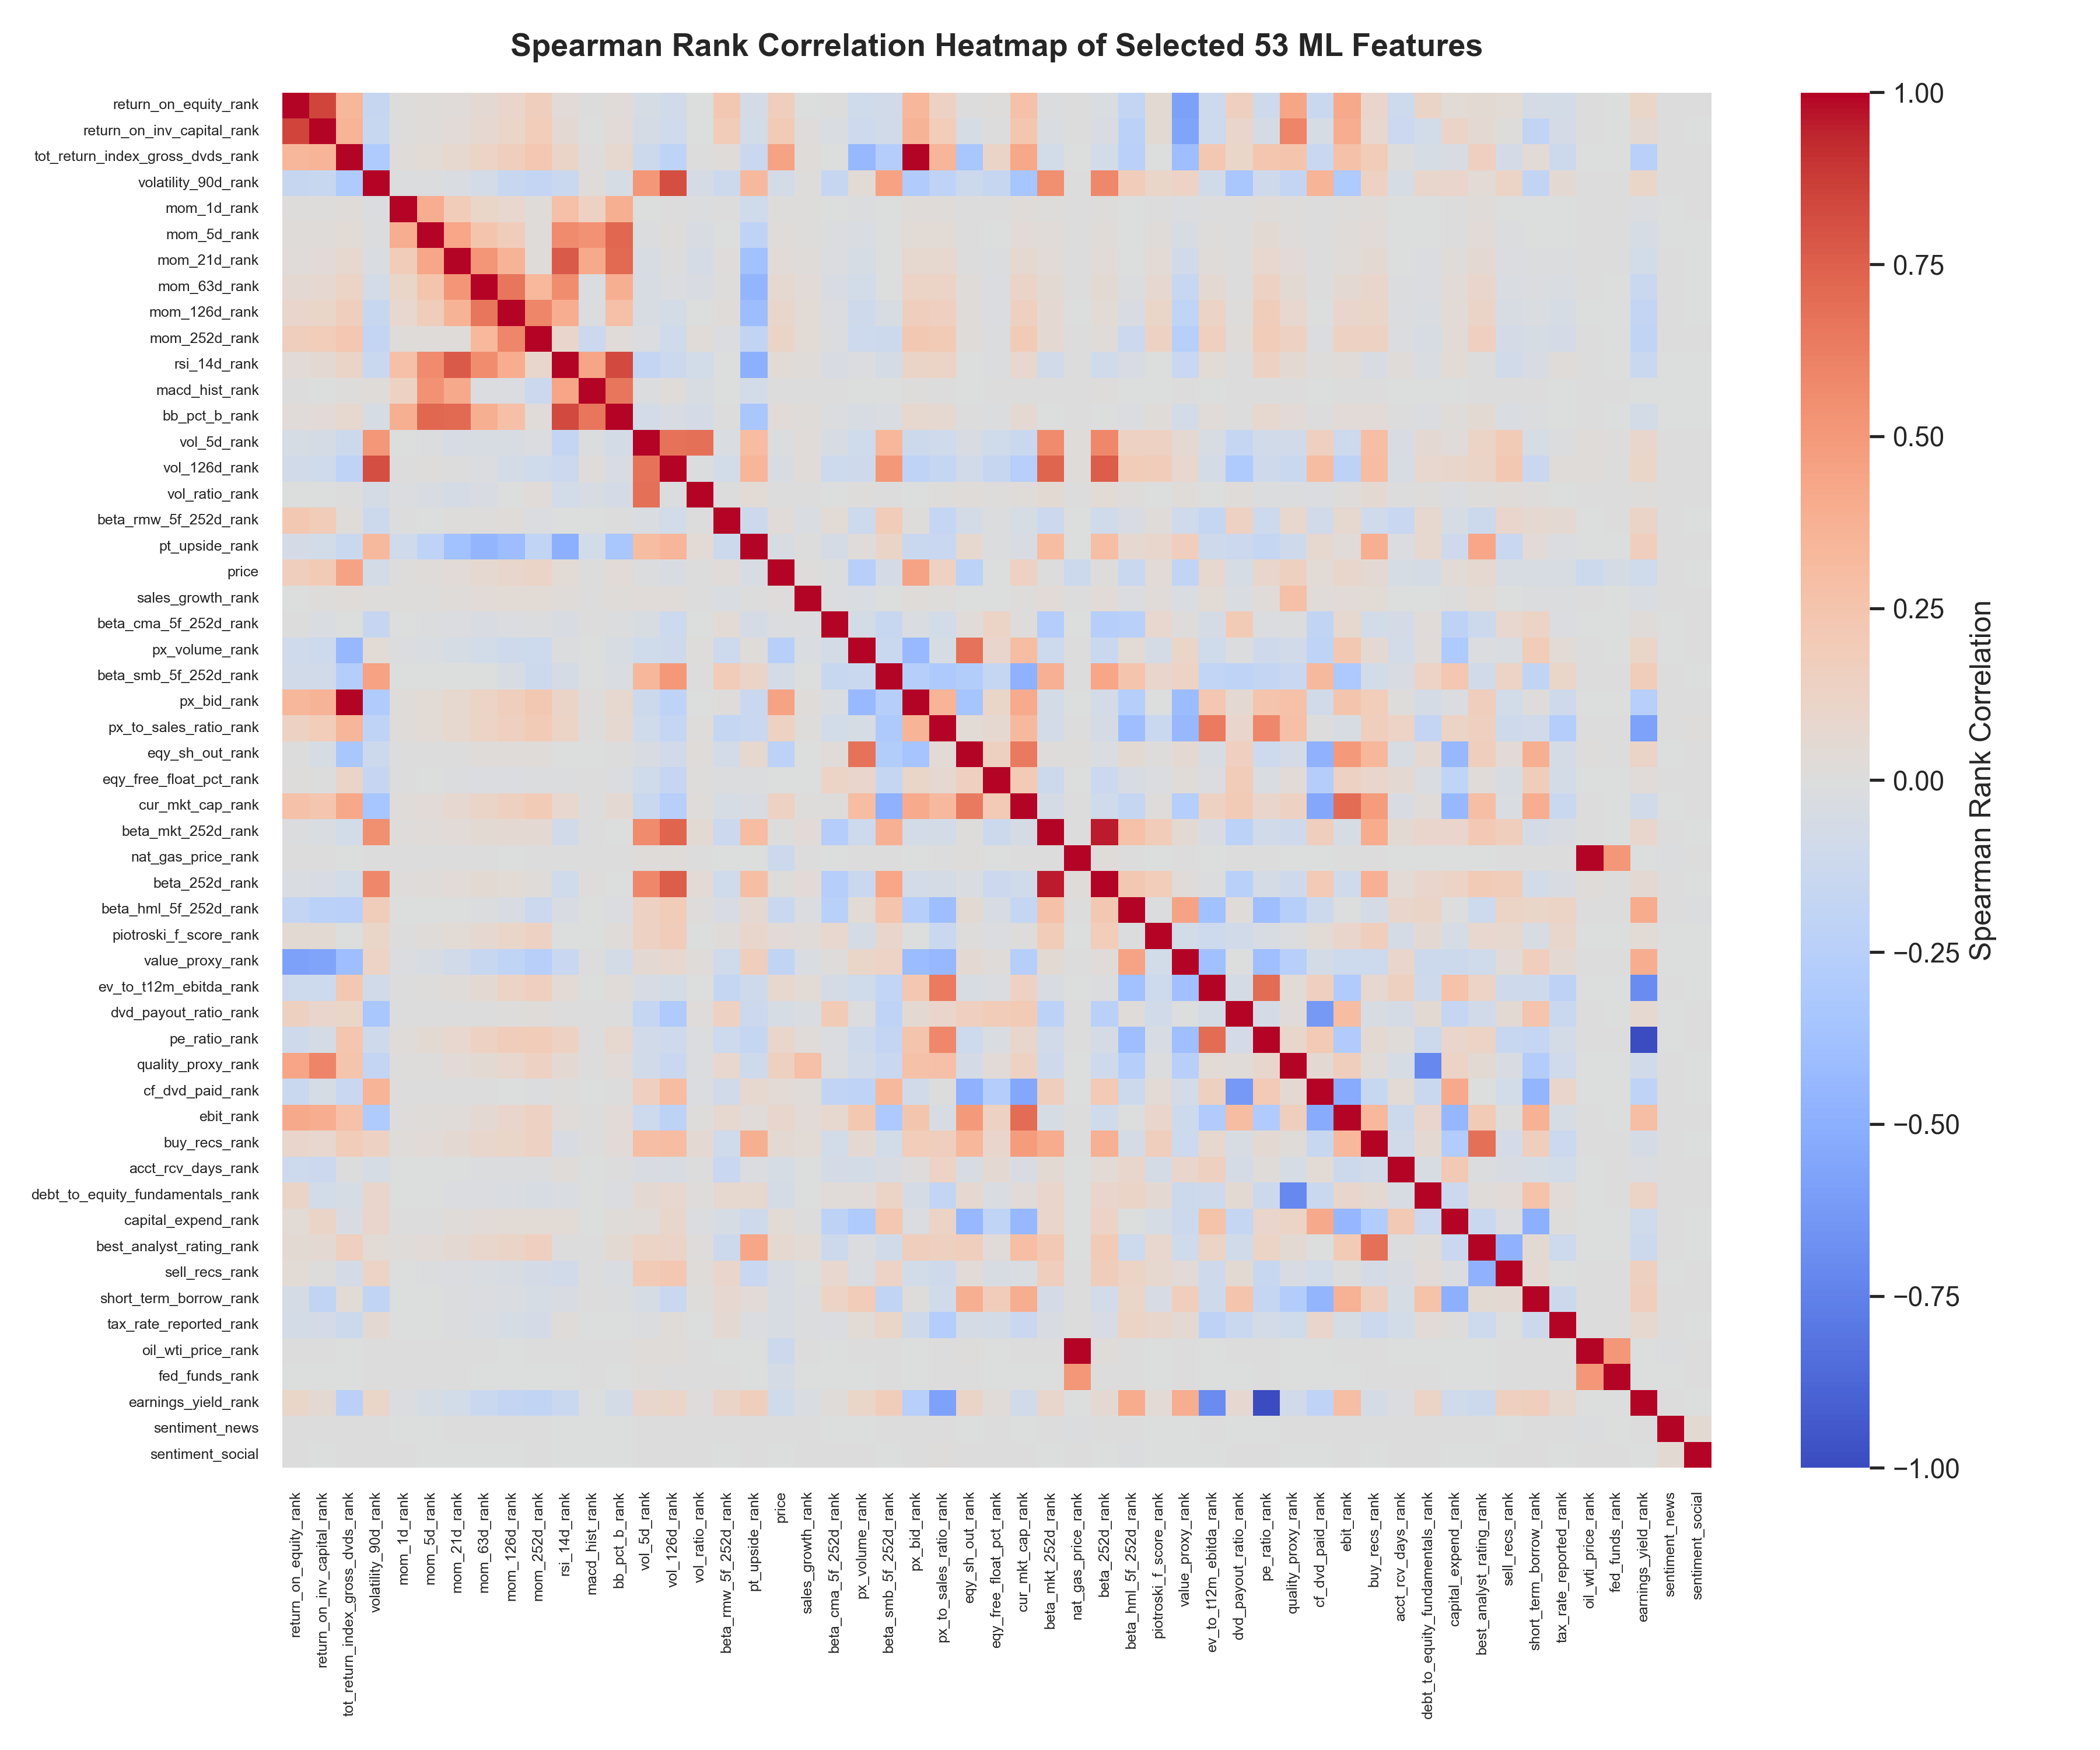
\includegraphics[width=0.82\textwidth]{./figures/selected_features_correlation.png}
\caption{Spearman Rank Correlation Heatmap of Selected 53 ML Features}
\label{fig:ch3_corr_heatmap}
\end{figure}

\begin{figure}[H]
\centering
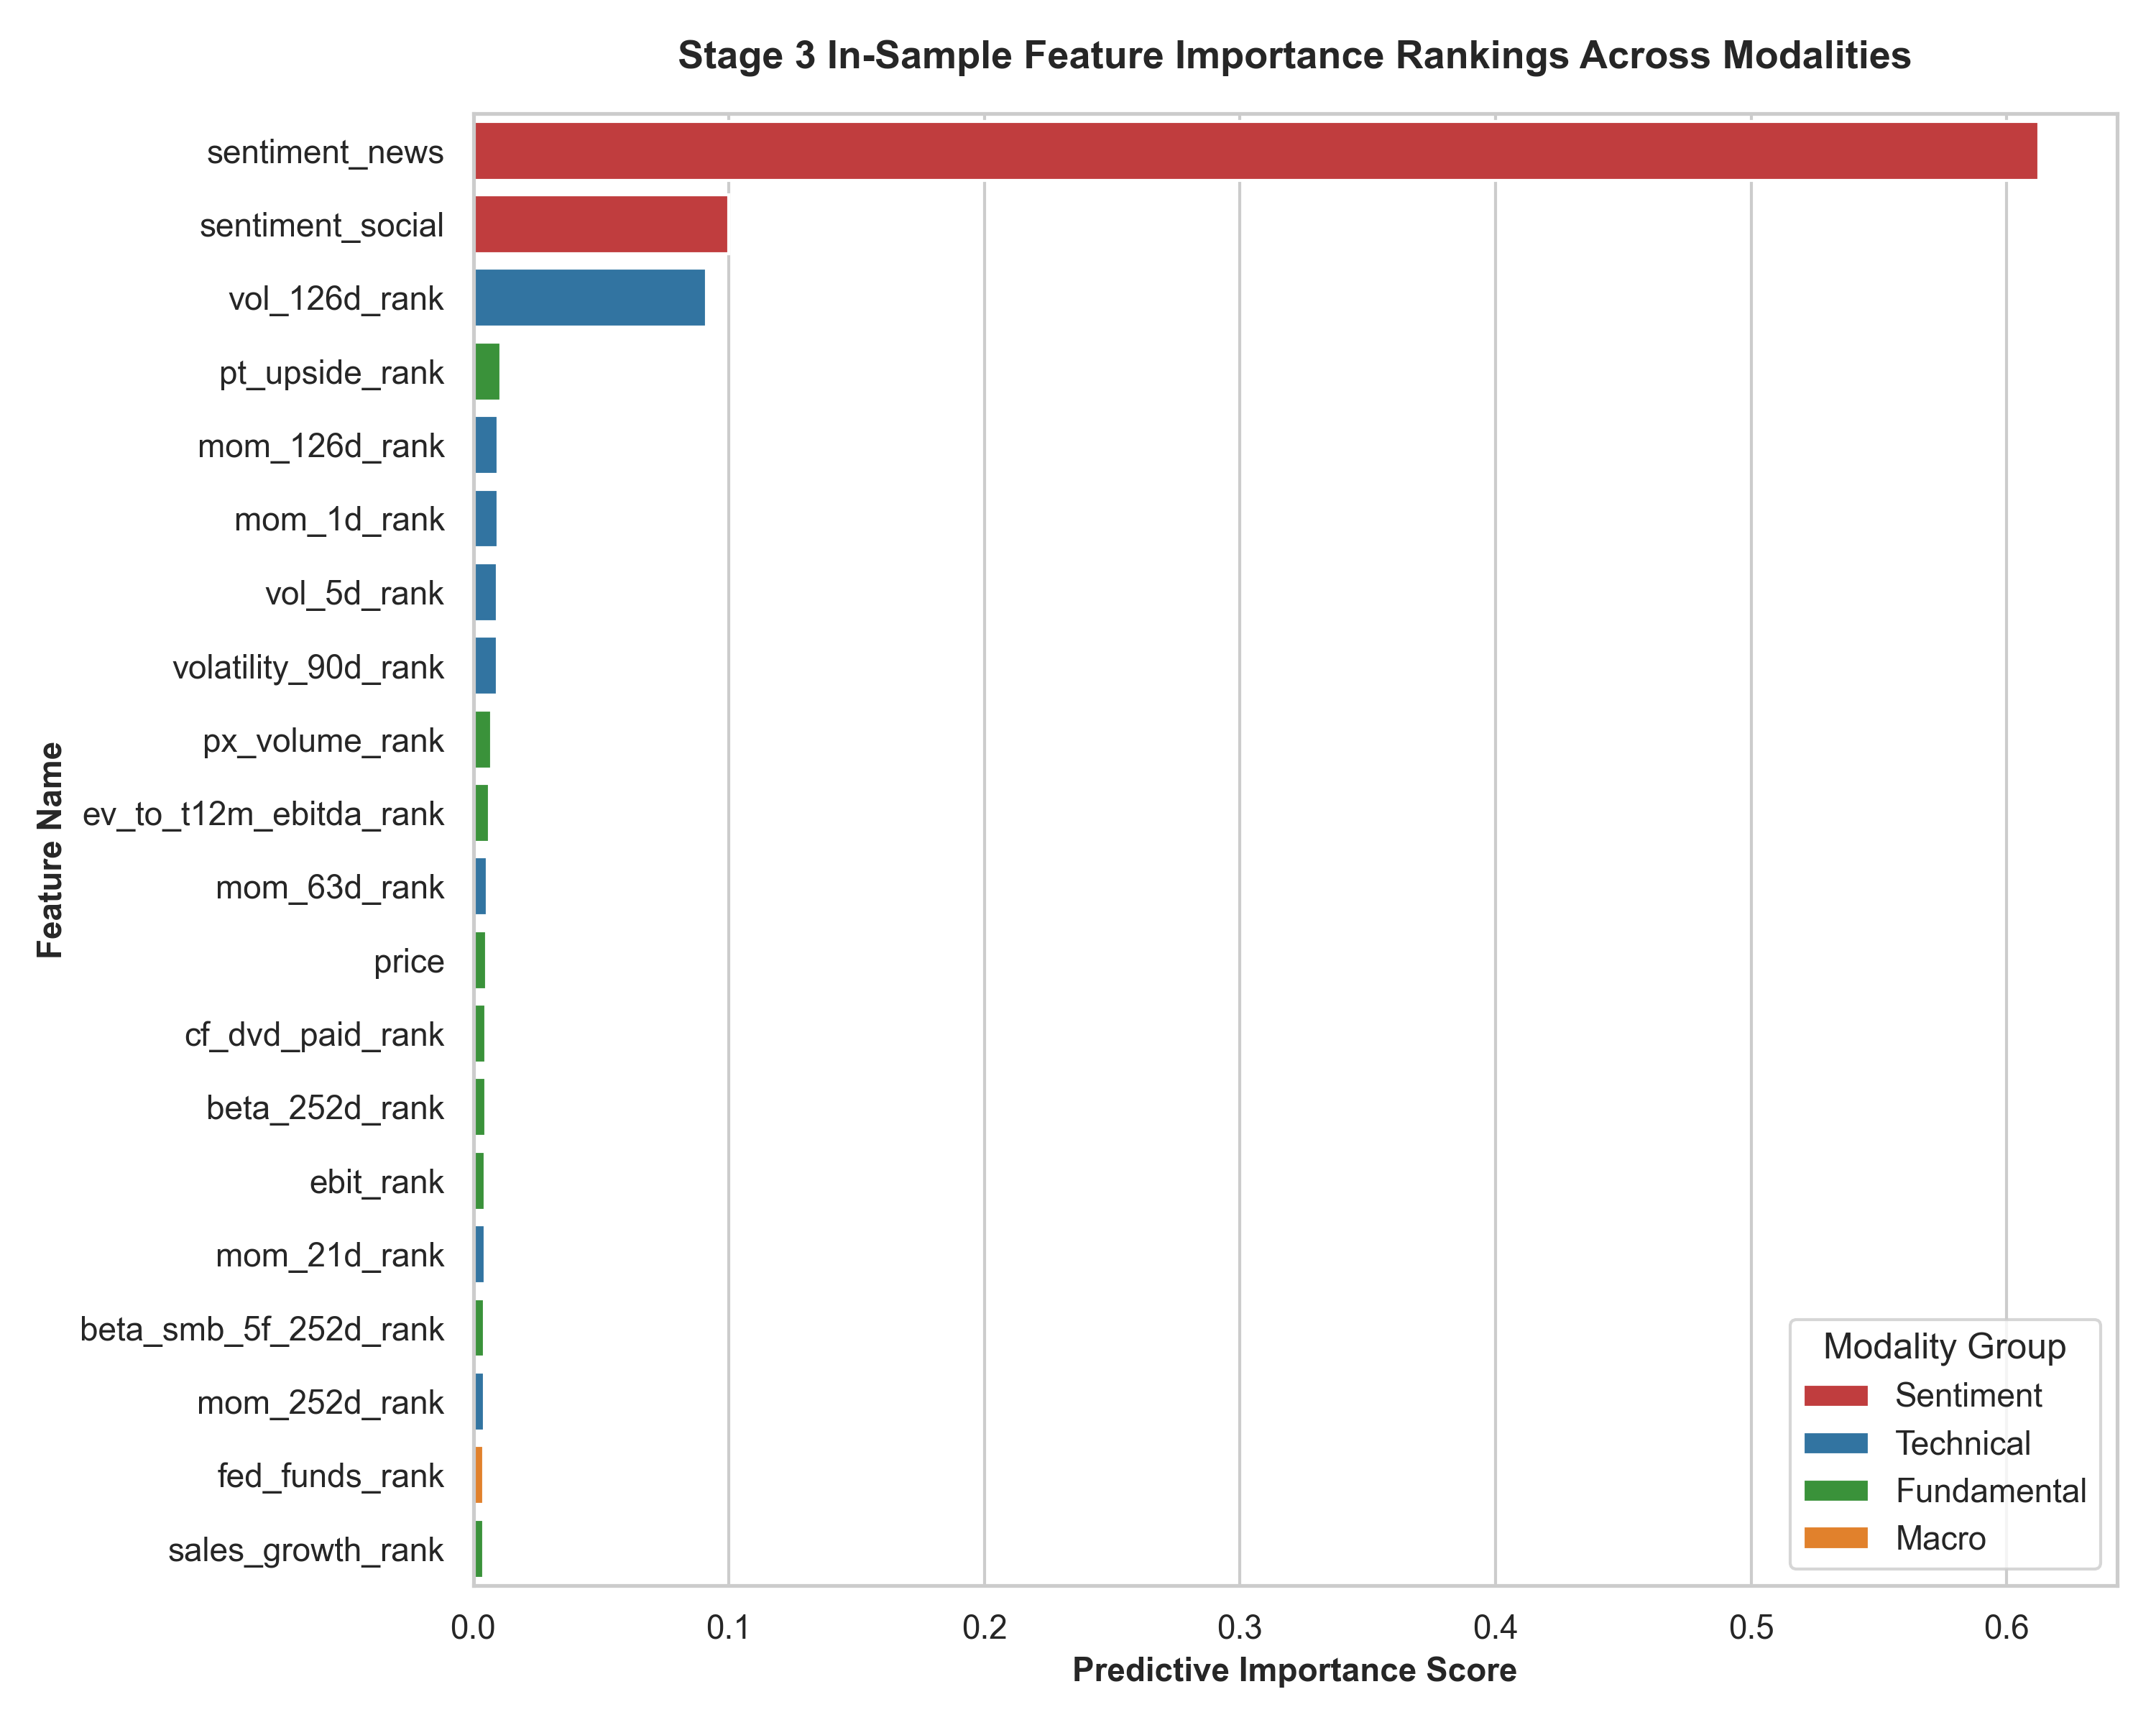
\includegraphics[width=0.82\textwidth]{./figures/selected_feature_importances.png}
\caption{Stage 3 Random Forest Feature Importance Rankings across Modalities}
\label{fig:ch3_rf_importance}
\end{figure}

% ,  END INPUT: data_and_features.tex , 


% ,  BEGIN INPUT: methodology.tex , 
\chapter{Methodology \& Model Architectures}
\label{ch:methodology}

\section{Introduction}
To evaluate whether nonlinear machine learning models and deep sequence architectures provide genuine predictive alpha over traditional factor pricing models in cross-sectional equity markets, we design an extensive econometric and deep learning methodology. The empirical model portfolio spans classical benchmark regressions, regularized linear shrinkage estimators, nonlinear decision tree ensembles, baseline recurrent sequence models, and a novel deep learning architecture: the \textbf{Temporal Fusion Deep Multimodal Gated Attention (TFDMGA)} network.

Predicting cross-sectional stock returns presents four fundamental econometric and algorithmic challenges:
\begin{enumerate}
    \item \textbf{High-Dimensionality and Multicollinearity}: Financial characteristics exhibit dense cross-sectional correlations, rendering unregularized ordinary least squares (OLS) highly unstable and prone to sample over-fitting.
    \item \textbf{Non-Linearity and Feature Interactions}: Factor interactions (e.g., momentum conditional on volatility or valuation conditional on market regime) are inherently nonlinear and difficult to specify \textit{a priori} using traditional parametric specifications.
    \item \textbf{Multimodal Heterogeneity}: Financial input signals originate from distinct modalities (technical price trends, fundamental accounting ratios, news sentiment indicators, and macroeconomic state variables) operating across differing sampling frequencies and dynamic noise regimes.
    \item \textbf{Macroeconomic Regime Sensitivity}: Dynamic factor risk premia vary across economic regimes (expansionary vs. contractionary, high vs. low market volatility), requiring adaptive model capacity capable of dynamically re-weighting predictive modalities.
\end{enumerate}

This chapter provides full step-by-step mathematical proofs and equation derivations for all baseline models and the TFDMGA architecture, details the 5-fold expanding-window walk-forward cross-validation protocol, describes the hyperparameter optimization methodology, and documents the computational resource execution profile.

\section{Baseline Econometric \& Machine Learning Formulations}
\label{sec:ch4_baselines}

To establish rigorous comparative benchmarks, we formulate four distinct model classes: linear factor regressions with robust covariance estimation, regularized linear shrinkage estimators, nonlinear tree ensembles, and recurrent neural network sequence encoders.

\subsection{Fama-MacBeth 2-Pass Linear Regression \& Newey-West HAC Estimation}
\label{subsec:ch4_fama_macbeth}

The benchmark linear asset pricing model follows the classic two-pass cross-sectional regression procedure of \citet{fama1973risk}, incorporating 1-day lagged factor loadings to eliminate lookahead bias and heteroskedasticity and autocorrelation consistent (HAC) covariance matrices \citep{newey1987simple}.

\subsubsection{Pass 1: Rolling Time-Series Factor Loading Estimation}
For each individual stock $i \in \{1, \dots, N_t\}$ on trading day $t$, factor loadings (betas) are estimated over a rolling historical lookback window of $W = 252$ trading days (one calendar year). Let $\mathbf{R}_{i,t} = [R_{i, t-W+1}, R_{i, t-W+2}, \dots, R_{i,t}]^T \in \mathbb{R}^{W \times 1}$ denote the vector of historical daily excess returns for asset $i$, and let $\mathbf{F}_t \in \mathbb{R}^{W \times (K+1)}$ represent the matrix of $K$ benchmark factor returns plus a column of ones for the intercept:
\begin{equation}
\mathbf{F}_t = \begin{bmatrix}
1 & F_{1, t-W+1} & F_{2, t-W+1} & \cdots & F_{K, t-W+1} \\
1 & F_{1, t-W+2} & F_{2, t-W+2} & \cdots & F_{K, t-W+2} \\
\vdots & \vdots & \vdots & \ddots & \vdots \\
1 & F_{1, t} & F_{2, t} & \cdots & F_{K, t}
\end{bmatrix}
\end{equation}

The first-pass time series Ordinary Least Squares (OLS) regression for stock $i$ is formulated as:
\begin{equation}
\mathbf{R}_{i,t} = \mathbf{F}_t \boldsymbol{\beta}_{i,t} + \boldsymbol{\epsilon}_{i,t}
\label{eq:ch4_pass1_ols}
\end{equation}
where $\boldsymbol{\beta}_{i,t} = [\alpha_{i,t}, \beta_{i,1,t}, \beta_{i,2,t}, \dots, \beta_{i,K,t}]^T \in \mathbb{R}^{(K+1) \times 1}$. The OLS point estimator is obtained by minimizing the sum of squared residuals:
\begin{equation}
\hat{\boldsymbol{\beta}}_{i,t} = \arg\min_{\boldsymbol{\beta}} (\mathbf{R}_{i,t} - \mathbf{F}_t \boldsymbol{\beta})^T (\mathbf{R}_{i,t} - \mathbf{F}_t \boldsymbol{\beta}) = \left( \mathbf{F}_t^T \mathbf{F}_t \right)^{-1} \mathbf{F}_t^T \mathbf{R}_{i,t}
\label{eq:ch4_beta_hat}
\end{equation}
To enforce strict zero-lookahead protection, factor loadings $\hat{\boldsymbol{\beta}}_{i,t}$ estimated using data strictly up to day $t$ are indexed to predict the realization of returns at day $t+1$.

\subsubsection{Pass 2: Daily Cross-Sectional Factor Risk Premia Estimation}
On each trading day $t+1$, a cross-sectional OLS regression is estimated across all active constituent assets $N_{t+1}$ using the 1-day lagged factor loadings $\hat{\mathbf{B}}_t = [\mathbf{1}, \hat{\boldsymbol{\beta}}_{1,t}, \hat{\boldsymbol{\beta}}_{2,t}, \dots, \hat{\boldsymbol{\beta}}_{N_{t+1},t}]^T \in \mathbb{R}^{N_{t+1} \times (K+1)}$:
\begin{equation}
\mathbf{R}_{t+1} = \hat{\mathbf{B}}_t \boldsymbol{\gamma}_{t+1} + \boldsymbol{\eta}_{t+1}
\label{eq:ch4_pass2_ols}
\end{equation}
where $\mathbf{R}_{t+1} = [R_{1,t+1}, R_{2,t+1}, \dots, R_{N_{t+1},t+1}]^T \in \mathbb{R}^{N_{t+1} \times 1}$ is the cross-section of realized forward returns, $\boldsymbol{\gamma}_{t+1} = [\gamma_{0,t+1}, \gamma_{1,t+1}, \dots, \gamma_{K,t+1}]^T \in \mathbb{R}^{(K+1) \times 1}$ represents the vector of daily factor risk premia (and cross-sectional intercept $\gamma_{0,t+1}$), and $\boldsymbol{\eta}_{t+1}$ is the vector of cross-sectional pricing errors.

The closed-form daily cross-sectional risk premium estimator is given by:
\begin{equation}
\hat{\boldsymbol{\gamma}}_{t+1} = \left( \hat{\mathbf{B}}_t^T \hat{\mathbf{B}}_t \right)^{-1} \hat{\mathbf{B}}_t^T \mathbf{R}_{t+1}
\label{eq:ch4_gamma_hat}
\end{equation}

\subsubsection{Time-Series Aggregation \& Step-by-Step Newey-West HAC Proof}
Over an evaluation period of $T$ trading days, the overall factor risk premium vector is estimated as the sample mean across daily cross-sectional estimates:
\begin{equation}
\bar{\boldsymbol{\gamma}} = \frac{1}{T} \sum_{t=1}^T \hat{\boldsymbol{\gamma}}_t
\end{equation}

Because daily factor risk premia estimates $\hat{\boldsymbol{\gamma}}_t$ suffer from serial correlation (autocorrelation) due to overlapping return measurement horizons and conditional heteroskedasticity in asset volatility, standard i.i.d. variance estimators severely underestimate true standard errors, inflating test statistics.

To derive a statistically consistent estimator for the asymptotic covariance matrix of $\bar{\boldsymbol{\gamma}}$, let $\mathbf{u}_t = \hat{\boldsymbol{\gamma}}_t - \bar{\boldsymbol{\gamma}} \in \mathbb{R}^{(K+1) \times 1}$ denote the vector of mean-zero risk premium innovations. The variance of the sample average factor risk premium is:
\begin{equation}
\operatorname{Var}(\bar{\boldsymbol{\gamma}}) = \operatorname{Var}\left( \frac{1}{T} \sum_{t=1}^T \hat{\boldsymbol{\gamma}}_t \right) = \frac{1}{T^2} \sum_{t=1}^T \sum_{s=1}^T \mathbb{E}\left[ \mathbf{u}_t \mathbf{u}_s^T \right]
\label{eq:ch4_var_gamma_sum}
\end{equation}
Defining the sample autocovariance matrix at lag $j$ as:
\begin{equation}
\hat{\mathbf{\Gamma}}_j = \frac{1}{T} \sum_{t=j+1}^T \mathbf{u}_t \mathbf{u}_{t-j}^T, \quad \text{for } j \ge 0
\label{eq:ch4_autocovariance}
\end{equation}
Equation (\ref{eq:ch4_var_gamma_sum}) can be expanded into the sum of zero-lag covariance and off-diagonal cross-lag covariances:
\begin{equation}
\operatorname{Var}(\bar{\boldsymbol{\gamma}}) = \frac{1}{T} \left[ \hat{\mathbf{\Gamma}}_0 + \sum_{j=1}^{T-1} \left( \hat{\mathbf{\Gamma}}_j + \hat{\mathbf{\Gamma}}_j^T \right) \right]
\end{equation}

Unweighted truncation of lag covariances at finite lag $L < T$ can lead to non-positive semi-definite covariance matrices in finite samples. The \citet{newey1987simple} HAC covariance matrix estimator guarantees positive semi-definiteness by weighting lag autocovariances with the triangular Bartlett kernel $w(j,L)$:
\begin{equation}
\widehat{\mathbf{\Omega}}_{\text{HAC}} = \hat{\mathbf{\Gamma}}_0 + \sum_{j=1}^L w(j, L) \left( \hat{\mathbf{\Gamma}}_j + \hat{\mathbf{\Gamma}}_j^T \right)
\label{eq:ch4_newey_west_omega}
\end{equation}
where the Bartlett kernel weights are defined as:
\begin{equation}
w(j, L) = 1 - \frac{j}{L+1}, \quad j = 1, 2, \dots, L
\label{eq:ch4_bartlett_kernel}
\end{equation}
and the optimal lag truncation bandwidth $L$ is set according to the automatic bandwidth selection rule $L = \lfloor 4 (T / 100)^{2/9} \rfloor$.

\begin{proof}[Proof of Guaranteed Positive Semi-Definiteness]
To prove that $\widehat{\mathbf{\Omega}}_{\text{HAC}} \succeq 0$, express the Bartlett kernel as the spectral window resulting from the convolution of a rectangular sequence with itself. Define $\mathbf{u}_t = \mathbf{0}$ for $t \notin \{1, \dots, T\}$. Consider the smoothed sequence $\mathbf{s}_t = \frac{1}{\sqrt{L+1}} \sum_{m=0}^L \mathbf{u}_{t+m}$. The sample covariance of $\mathbf{s}_t$ is manifestly positive semi-definite:
\begin{align}
\mathbf{M} &= \frac{1}{T} \sum_{t=-\infty}^{\infty} \mathbf{s}_t \mathbf{s}_t^T = \frac{1}{T(L+1)} \sum_{t=-\infty}^{\infty} \left( \sum_{m=0}^L \mathbf{u}_{t+m} \right) \left( \sum_{n=0}^L \mathbf{u}_{t+n}^T \right) \ge 0
\end{align}
Expanding the double summation yields:
\begin{align}
\mathbf{M} &= \frac{1}{T(L+1)} \sum_{m=0}^L \sum_{n=0}^L \sum_{t=-\infty}^{\infty} \mathbf{u}_{t+m} \mathbf{u}_{t+n}^T = \frac{1}{T(L+1)} \sum_{m=0}^L \sum_{n=0}^L T \hat{\mathbf{\Gamma}}_{m-n} \\
&= \frac{1}{L+1} \sum_{k=-L}^L (L + 1 - |k|) \hat{\mathbf{\Gamma}}_k = \hat{\mathbf{\Gamma}}_0 + \sum_{j=1}^L \left( 1 - \frac{j}{L+1} \right) \left( \hat{\mathbf{\Gamma}}_j + \hat{\mathbf{\Gamma}}_j^T \right) = \widehat{\mathbf{\Omega}}_{\text{HAC}}
\end{align}
Since $\mathbf{M}$ is constructed as a sum of outer products $\mathbf{s}_t \mathbf{s}_t^T$, for any vector $\mathbf{a} \in \mathbb{R}^{K+1}$, $\mathbf{a}^T \widehat{\mathbf{\Omega}}_{\text{HAC}} \mathbf{a} = \frac{1}{T} \sum_t (\mathbf{a}^T \mathbf{s}_t)^2 \ge 0$. Thus, $\widehat{\mathbf{\Omega}}_{\text{HAC}}$ is strictly positive semi-definite.
\end{proof}

The Newey-West adjusted standard error for the $k$-th factor risk premium estimate $\bar{\gamma}_k$ is:
\begin{equation}
\text{SE}_{\text{NW}}(\bar{\gamma}_k) = \sqrt{ \frac{1}{T} \left[ \widehat{\mathbf{\Omega}}_{\text{HAC}} \right]_{kk} }
\end{equation}
and the robust test statistic for factor significance testing is evaluated as $t(\bar{\gamma}_k) = \frac{\bar{\gamma}_k}{\text{SE}_{\text{NW}}(\bar{\gamma}_k)}$.

\subsection{Regularized Linear Models: ElasticNet, LASSO, \& Ridge}
\label{subsec:ch4_elasticnet_lasso_ridge}

High dimensional cross-sectional asset pricing settings with $P$ characteristic features suffer from severe multicollinearity and sample over-fitting under standard OLS. Regularized linear models introduce penalization structures to constrain coefficient magnitudes and perform feature selection \citep{kozak2020shrinking}.

\subsubsection{ElasticNet Objective Function}
Let $\mathbf{y} \in \mathbb{R}^N$ denote the vector of standardized forward returns across all asset-day observations, and let $\mathbf{X} \in \mathbb{R}^{N \times P}$ denote the matrix of standardized stock characteristics. The ElasticNet estimator \citep{zou2005regularization} solves the convex optimization problem:
\begin{equation}
\min_{\boldsymbol{\beta} \in \mathbb{R}^P} \mathcal{L}_{\text{EN}}(\boldsymbol{\beta}) = \frac{1}{2N} \|\mathbf{y} - \mathbf{X}\boldsymbol{\beta}\|_2^2 + \lambda \left[ \alpha \|\boldsymbol{\beta}\|_1 + \frac{1-\alpha}{2} \|\boldsymbol{\beta}\|_2^2 \right]
\label{eq:ch4_elasticnet_full}
\end{equation}
where $\lambda > 0$ controls the overall penalty intensity, $\alpha \in [0, 1]$ governs the ratio between the $L_1$ norm $\|\boldsymbol{\beta}\|_1 = \sum_{j=1}^P |\beta_j|$ and the squared $L_2$ norm $\|\boldsymbol{\beta}\|_2^2 = \sum_{j=1}^P \beta_j^2$. Setting $\alpha = 1.0$ yields the pure LASSO estimator \citep{tibshirani1996regression}, while $\alpha = 0.0$ yields Ridge regression \citep{hoerl1970ridge}.

\subsubsection{Subgradient Calculus \& Characterization of LASSO ($L_1$) Sparsity}
Because the $L_1$ norm is non-differentiable at $\beta_j = 0$, optimization requires subgradient calculus. The subdifferential $\partial |\beta_j|$ of the absolute value function is defined as:
\begin{equation}
\partial |\beta_j| = \begin{cases} 
\{ +1 \} & \text{if } \beta_j > 0 \\
\{ -1 \} & \text{if } \beta_j < 0 \\
[-1, 1] & \text{if } \beta_j = 0 
\end{cases}
\label{eq:ch4_subgradient_l1}
\end{equation}

To derive the coordinate descent update rule for feature $j$, assume without loss of generality that the columns of $\mathbf{X}$ are standardized such that $\mathbf{x}_j^T \mathbf{x}_j = N$. Isolate feature $j$ by defining the partial residual vector $\mathbf{r}^{(j)} = \mathbf{y} - \sum_{k \neq j} \mathbf{x}_k \beta_k$. The unregularized OLS update for $\beta_j$ given fixed $\boldsymbol{\beta}_{-j}$ is $\hat{\beta}_j^{\text{OLS}} = \frac{1}{N} \mathbf{x}_j^T \mathbf{r}^{(j)}$.

The first order optimality condition for the ElasticNet objective requires $0 \in \partial_{\beta_j} \mathcal{L}_{\text{EN}}(\boldsymbol{\beta})$:
\begin{equation}
-\frac{1}{N} \mathbf{x}_j^T (\mathbf{y} - \mathbf{X}\boldsymbol{\beta}) + \lambda(1-\alpha)\beta_j + \lambda \alpha v_j = 0, \quad \text{where } v_j \in \partial |\beta_j|
\end{equation}
Substituting $\mathbf{y} - \mathbf{X}\boldsymbol{\beta} = \mathbf{r}^{(j)} - \mathbf{x}_j \beta_j$ and using $\frac{1}{N}\mathbf{x}_j^T \mathbf{x}_j = 1$:
\begin{equation}
-\hat{\beta}_j^{\text{OLS}} + \beta_j + \lambda(1-\alpha)\beta_j + \lambda \alpha v_j = 0 \implies \beta_j [ 1 + \lambda(1-\alpha) ] + \lambda \alpha v_j = \hat{\beta}_j^{\text{OLS}}
\label{eq:ch4_opt_condition}
\end{equation}

Solving Equation (\ref{eq:ch4_opt_condition}) under three case conditions for $\hat{\beta}_j^{\text{OLS}}$:
\begin{enumerate}
    \item \textbf{Case 1: $\beta_j > 0$}. Here $v_j = +1$. Equation (\ref{eq:ch4_opt_condition}) gives $\beta_j [1 + \lambda(1-\alpha)] = \hat{\beta}_j^{\text{OLS}} - \lambda \alpha$, requiring $\hat{\beta}_j^{\text{OLS}} > \lambda \alpha$. Thus:
    $$\beta_j^* = \frac{\hat{\beta}_j^{\text{OLS}} - \lambda \alpha}{1 + \lambda(1-\alpha)}$$
    \item \textbf{Case 2: $\beta_j < 0$}. Here $v_j = -1$. Equation (\ref{eq:ch4_opt_condition}) gives $\beta_j [1 + \lambda(1-\alpha)] = \hat{\beta}_j^{\text{OLS}} + \lambda \alpha$, requiring $\hat{\beta}_j^{\text{OLS}} < -\lambda \alpha$. Thus:
    $$\beta_j^* = \frac{\hat{\beta}_j^{\text{OLS}} + \lambda \alpha}{1 + \lambda(1-\alpha)}$$
    \item \textbf{Case 3: $\beta_j = 0$}. Here $v_j \in [-1, 1]$. Equation (\ref{eq:ch4_opt_condition}) requires $|\hat{\beta}_j^{\text{OLS}}| \le \lambda \alpha$. Thus, $\beta_j^* = 0$.
\end{enumerate}

Combining these cases yields the closed-form Soft-Thresholding Operator $\mathcal{S}_{\kappa}(z) = \operatorname{sign}(z) \max(0, |z| - \kappa)$:
\begin{equation}
\hat{\beta}_j^{\text{EN}} = \frac{\mathcal{S}_{\lambda \alpha}\left( \hat{\beta}_j^{\text{OLS}} \right)}{1 + \lambda (1-\alpha)}
\label{eq:ch4_soft_thresholding_en}
\end{equation}
Setting $\alpha = 1.0$ yields the standard LASSO soft-thresholded estimator $\hat{\beta}_j^{\text{LASSO}} = \mathcal{S}_{\lambda}\left( \hat{\beta}_j^{\text{OLS}} \right)$, which explicitly forces coefficients to zero whenever $|\hat{\beta}_j^{\text{OLS}}| \le \lambda$, executing exact feature selection.

\subsubsection{Ridge ($L_2$) Shrinkage Bounds \& SVD Derivation}
For pure Ridge regression ($\alpha = 0$), the objective function is smooth and differentiable. Differentiating $\mathcal{L}_{\text{Ridge}}(\boldsymbol{\beta})$ with respect to $\boldsymbol{\beta}$ yields the closed-form Ridge estimator:
\begin{equation}
\hat{\boldsymbol{\beta}}_{\text{Ridge}} = \left( \mathbf{X}^T \mathbf{X} + N \lambda \mathbf{I}_P \right)^{-1} \mathbf{X}^T \mathbf{y}
\label{eq:ch4_ridge_closed_form}
\end{equation}

To prove strict $L_2$ shrinkage bounds, consider the Singular Value Decomposition (SVD) of the centered design matrix $\mathbf{X} = \mathbf{U} \mathbf{\Sigma} \mathbf{V}^T$, where $\mathbf{U} \in \mathbb{R}^{N \times P}$ and $\mathbf{V} \in \mathbb{R}^{P \times P}$ are orthonormal matrices ($\mathbf{U}^T \mathbf{U} = \mathbf{I}_P$, $\mathbf{V}^T \mathbf{V} = \mathbf{I}_P$), and $\mathbf{\Sigma} = \operatorname{diag}(\sigma_1, \sigma_2, \dots, \sigma_P)$ contains the singular values $\sigma_1 \ge \sigma_2 \ge \dots \ge \sigma_P > 0$.

Substituting the SVD into the standard OLS estimator $\hat{\boldsymbol{\beta}}_{\text{OLS}} = (\mathbf{X}^T \mathbf{X})^{-1} \mathbf{X}^T \mathbf{y}$:
\begin{equation}
\hat{\boldsymbol{\beta}}_{\text{OLS}} = \left( \mathbf{V} \mathbf{\Sigma}^2 \mathbf{V}^T \right)^{-1} \mathbf{V} \mathbf{\Sigma} \mathbf{U}^T \mathbf{y} = \mathbf{V} \mathbf{\Sigma}^{-1} \mathbf{U}^T \mathbf{y}
\end{equation}

Substituting the SVD into the Ridge estimator Equation (\ref{eq:ch4_ridge_closed_form}):
\begin{align}
\hat{\boldsymbol{\beta}}_{\text{Ridge}} &= \left( \mathbf{V} \mathbf{\Sigma}^2 \mathbf{V}^T + N \lambda \mathbf{V} \mathbf{I}_P \mathbf{V}^T \right)^{-1} \mathbf{V} \mathbf{\Sigma} \mathbf{U}^T \mathbf{y} \\
&= \left( \mathbf{V} [ \mathbf{\Sigma}^2 + N \lambda \mathbf{I}_P ] \mathbf{V}^T \right)^{-1} \mathbf{V} \mathbf{\Sigma} \mathbf{U}^T \mathbf{y} \\
&= \mathbf{V} \left( \mathbf{\Sigma}^2 + N \lambda \mathbf{I}_P \right)^{-1} \mathbf{\Sigma} \mathbf{U}^T \mathbf{y}
\label{eq:ch4_ridge_svd}
\end{align}

Expressing $\hat{\boldsymbol{\beta}}_{\text{Ridge}}$ directly as a transformation of the unregularized OLS estimator $\hat{\boldsymbol{\beta}}_{\text{OLS}}$:
\begin{align}
\hat{\boldsymbol{\beta}}_{\text{Ridge}} &= \mathbf{V} \left( \mathbf{\Sigma}^2 + N \lambda \mathbf{I}_P \right)^{-1} \mathbf{\Sigma}^2 \mathbf{\Sigma}^{-1} \mathbf{U}^T \mathbf{y} \\
&= \mathbf{V} \operatorname{diag}\left( \frac{\sigma_j^2}{\sigma_j^2 + N \lambda} \right) \mathbf{V}^T \hat{\boldsymbol{\beta}}_{\text{OLS}}
\label{eq:ch4_ridge_shrinkage_matrix}
\end{align}

Because $N \lambda > 0$ and $\sigma_j^2 > 0$, the shrinkage factor satisfies:
\begin{equation}
0 < \frac{\sigma_j^2}{\sigma_j^2 + N \lambda} < 1, \quad \forall j \in \{1, \dots, P\}
\end{equation}
This proves that Ridge regression strictly shrinks the OLS parameter vector along the principal component directions of $\mathbf{X}$, with greater shrinkage applied to minor components with smaller singular values $\sigma_j^2$. Consequently, $\|\hat{\boldsymbol{\beta}}_{\text{Ridge}}\|_2 < \|\hat{\boldsymbol{\beta}}_{\text{OLS}}\|_2$ for all $\lambda > 0$, bounding parameter variance and stabilizing prediction in the presence of severe collinearity.

\subsection{Non-Linear Tree Ensembles: Random Forest \& XGBoost}
\label{subsec:ch4_tree_ensembles}

Decision tree ensembles non-parametrically map high dimensional characteristic spaces into predicted returns by partitioning features into hyper-rectangular regions \citep{gu2020empirical}.

\subsubsection{Random Forest Bagging Variance Reduction Proof}
The Random Forest regressor \citep{breiman2001random} constructs an ensemble of $M$ decorrelated decision trees $\{T_1(\mathbf{x}), T_2(\mathbf{x}), \dots, T_M(\mathbf{x})\}$, each trained on a distinct bootstrap sample of size $N$ with randomized feature subspace selection ($m_{\text{try}} = \lfloor \sqrt{P} \rfloor$). The ensemble prediction is the arithmetic mean:
\begin{equation}
\hat{f}_{\text{RF}}(\mathbf{x}) = \frac{1}{M} \sum_{m=1}^M T_m(\mathbf{x})
\label{eq:ch4_rf_prediction}
\end{equation}

Assume each individual tree $T_m(\mathbf{x})$ is identically distributed with variance $\operatorname{Var}(T_m(\mathbf{x})) = \sigma^2$, and that any pair of distinct trees $(T_m, T_l)$ for $m \neq l$ has pairwise correlation $\text{Corr}(T_m(\mathbf{x}), T_l(\mathbf{x})) = \rho$.

\begin{proof}[Proof of Variance Reduction Dynamics]
Compute the variance of the ensemble estimator $\hat{f}_{\text{RF}}(\mathbf{x})$:
\begin{align}
\operatorname{Var}\left( \hat{f}_{\text{RF}}(\mathbf{x}) \right) &= \operatorname{Var}\left( \frac{1}{M} \sum_{m=1}^M T_m(\mathbf{x}) \right) \\
&= \frac{1}{M^2} \left[ \sum_{m=1}^M \operatorname{Var}(T_m(\mathbf{x})) + \sum_{m=1}^M \sum_{l \neq m}^M \operatorname{Cov}(T_m(\mathbf{x}), T_l(\mathbf{x})) \right]
\label{eq:ch4_var_rf_expansion}
\end{align}
Substitute $\operatorname{Var}(T_m(\mathbf{x})) = \sigma^2$ and $\operatorname{Cov}(T_m(\mathbf{x}), T_l(\mathbf{x})) = \rho \sigma^2$:
\begin{align}
\operatorname{Var}\left( \hat{f}_{\text{RF}}(\mathbf{x}) \right) &= \frac{1}{M^2} \left[ M \sigma^2 + M(M-1) \rho \sigma^2 \right] \\
&= \frac{\sigma^2}{M} + \frac{M-1}{M} \rho \sigma^2 = \rho \sigma^2 + \frac{1 - \rho}{M} \sigma^2
\label{eq:ch4_var_rf_final}
\end{align}
\end{proof}

Taking the limit as the number of trees $M \to \infty$:
\begin{equation}
\lim_{M \to \infty} \operatorname{Var}\left( \hat{f}_{\text{RF}}(\mathbf{x}) \right) = \rho \sigma^2
\end{equation}
Equation (\ref{eq:ch4_var_rf_final}) demonstrates the dual variance-reduction mechanism of Random Forest:
\begin{enumerate}
    \item \textbf{Bagging} (bootstrap aggregation) drives the second term $\frac{1-\rho}{M} \sigma^2$ to zero by increasing ensemble size $M$.
    \item \textbf{Random Feature Subspace Selection} reduces inter-tree correlation $\rho$, lowering the asymptotic variance floor $\rho \sigma^2$.
\end{enumerate}

\subsubsection{XGBoost Second-Order Taylor Expansion Loss Optimization}
Extreme Gradient Boosting (XGBoost) \citep{chen2016xgboost} builds an additive model of $M$ decision trees sequentially: $\hat{y}_i^{(m)} = \hat{y}_i^{(m-1)} + f_m(\mathbf{x}_i)$. At step $m$, the regularized objective function to minimize is:
\begin{equation}
\mathcal{L}^{(m)} = \sum_{i=1}^N l\left( y_i, \hat{y}_i^{(m-1)} + f_m(\mathbf{x}_i) \right) + \Omega(f_m)
\label{eq:ch4_xgb_obj}
\end{equation}
where $l(\cdot, \cdot)$ is a differentiable convex loss function, and the tree complexity regularization term $\Omega(f_m)$ is defined for a tree with $T$ leaf nodes and leaf weight vector $\mathbf{w} = [w_1, \dots, w_T]^T \in \mathbb{R}^T$ as:
\begin{equation}
\Omega(f_m) = \gamma T + \frac{1}{2} \lambda \|\mathbf{w}\|_2^2 = \gamma T + \frac{1}{2} \lambda \sum_{j=1}^T w_j^2
\label{eq:ch4_xgb_reg}
\end{equation}

Applying a second order Taylor expansion to the loss function around the previous iteration step forecast $\hat{y}_i^{(m-1)}$:
\begin{equation}
l\left( y_i, \hat{y}_i^{(m-1)} + f_m(\mathbf{x}_i) \right) \approx l\left( y_i, \hat{y}_i^{(m-1)} \right) + g_i f_m(\mathbf{x}_i) + \frac{1}{2} h_i f_m(\mathbf{x}_i)^2
\label{eq:ch4_taylor_loss}
\end{equation}
where the first order gradient $g_i$ and second order Hessian $h_i$ are defined as:
\begin{equation}
g_i = \frac{\partial l\left( y_i, \hat{y}_i^{(m-1)} \right)}{\partial \hat{y}_i^{(m-1)}}, \quad h_i = \frac{\partial^2 l\left( y_i, \hat{y}_i^{(m-1)} \right)}{\partial \left(\hat{y}_i^{(m-1)}\right)^2}
\label{eq:ch4_grad_hessian}
\end{equation}

Removing constant terms $l(y_i, \hat{y}_i^{(m-1)})$ independent of tree structure $f_m$, the simplified objective at step $m$ becomes:
\begin{equation}
\tilde{\mathcal{L}}^{(m)} = \sum_{i=1}^N \left[ g_i f_m(\mathbf{x}_i) + \frac{1}{2} h_i f_m(\mathbf{x}_i)^2 \right] + \gamma T + \frac{1}{2} \lambda \sum_{j=1}^T w_j^2
\label{eq:ch4_xgb_simplified_obj}
\end{equation}

Let $I_j = \{i \mid q(\mathbf{x}_i) = j\}$ represent the instance set mapped to leaf node $j$ by structure mapping function $q: \mathbb{R}^P \to \{1, \dots, T\}$. Rewriting the summation across individual samples $i$ as a summation over leaf nodes $j$:
\begin{equation}
\tilde{\mathcal{L}}^{(m)} = \sum_{j=1}^T \left[ \left( \sum_{i \in I_j} g_i \right) w_j + \frac{1}{2} \left( \sum_{i \in I_j} h_i + \lambda \right) w_j^2 \right] + \gamma T
\label{eq:ch4_xgb_grouped_obj}
\end{equation}

Define aggregate leaf gradient $G_j = \sum_{i \in I_j} g_i$ and aggregate leaf Hessian $H_j = \sum_{i \in I_j} h_i$:
\begin{equation}
\tilde{\mathcal{L}}^{(m)} = \sum_{j=1}^T \left[ G_j w_j + \frac{1}{2} (H_j + \lambda) w_j^2 \right] + \gamma T
\end{equation}

Taking the partial derivative of $\tilde{\mathcal{L}}^{(m)}$ with respect to weight $w_j$ and setting it to zero yields the optimal weight $w_j^*$ for leaf $j$:
\begin{equation}
\frac{\partial \tilde{\mathcal{L}}^{(m)}}{\partial w_j} = G_j + (H_j + \lambda) w_j = 0 \implies w_j^* = -\frac{G_j}{H_j + \lambda}
\label{eq:ch4_xgb_optimal_w}
\end{equation}

Substituting $w_j^*$ back into the objective yields the optimal minimized loss value (tree structure quality score):
\begin{equation}
\tilde{\mathcal{L}}^{(m)*} = -\frac{1}{2} \sum_{j=1}^T \frac{G_j^2}{H_j + \lambda} + \gamma T
\label{eq:ch4_xgb_structure_score}
\end{equation}

When evaluating candidate node splits during tree construction, the gain score for splitting a node into left instance subset $I_L$ and right instance subset $I_R$ is evaluated as:
\begin{equation}
\operatorname{Gain} = \frac{1}{2} \left[ \frac{G_L^2}{H_L + \lambda} + \frac{G_R^2}{H_R + \lambda} - \frac{(G_L + G_R)^2}{H_L + H_R + \lambda} \right] - \gamma
\label{eq:ch4_xgb_gain}
\end{equation}
where $\gamma$ acts as a penalty threshold requiring the improvement in loss reduction to exceed $\gamma$ before authorizing a node split.

\subsection{Baseline Sequence Encoder: PyTorch LSTM}
\label{subsec:ch4_lstm}

To encode temporal patterns across a sequential lookback window of $T = 20$ trading days, we deploy a multilayer Long Short-Term Memory (LSTM) network \citep{hochreiter1997long}.

For input vector $\mathbf{x}_t \in \mathbb{R}^{d_{\text{in}}}$ at sequence step $t \in \{1, \dots, T\}$, previous hidden state $\mathbf{h}_{t-1} \in \mathbb{R}^D$, and previous cell state $\mathbf{c}_{t-1} \in \mathbb{R}^D$, the PyTorch LSTM cell execution equations are formulated as:
\begin{align}
\mathbf{i}_t &= \sigma\left( \mathbf{W}_{xi} \mathbf{x}_t + \mathbf{W}_{hi} \mathbf{h}_{t-1} + \mathbf{b}_{ii} + \mathbf{b}_{hi} \right) \quad &&\text{(Input Gate)} \label{eq:ch4_lstm_input_gate} \\
\mathbf{f}_t &= \sigma\left( \mathbf{W}_{xf} \mathbf{x}_t + \mathbf{W}_{hf} \mathbf{h}_{t-1} + \mathbf{b}_{if} + \mathbf{b}_{hf} \right) \quad &&\text{(Forget Gate)} \label{eq:ch4_lstm_forget_gate} \\
\mathbf{o}_t &= \sigma\left( \mathbf{W}_{xo} \mathbf{x}_t + \mathbf{W}_{ho} \mathbf{h}_{t-1} + \mathbf{b}_{io} + \mathbf{b}_{ho} \right) \quad &&\text{(Output Gate)} \label{eq:ch4_lstm_output_gate} \\
\tilde{\mathbf{c}}_t &= \tanh\left( \mathbf{W}_{xc} \mathbf{x}_t + \mathbf{W}_{hc} \mathbf{h}_{t-1} + \mathbf{b}_{ic} + \mathbf{b}_{hc} \right) \quad &&\text{(Cell Candidate)} \label{eq:ch4_lstm_cell_cand} \\
\mathbf{c}_t &= \mathbf{f}_t \odot \mathbf{c}_{t-1} + \mathbf{i}_t \odot \tilde{\mathbf{c}}_t \quad &&\text{(Cell State Update)} \label{eq:ch4_lstm_cell_update} \\
\mathbf{h}_t &= \mathbf{o}_t \odot \tanh(\mathbf{c}_t) \quad &&\text{(Hidden State Output)} \label{eq:ch4_lstm_hidden_update}
\end{align}
where $\sigma(z) = (1 + e^{-z})^{-1}$ is the element-wise logistic sigmoid function, $\tanh(z) = \frac{e^z - e^{-z}}{e^z + e^{-z}}$ is the hyperbolic tangent activation, and $\odot$ represents the Hadamard (element-wise) product. Weight matrices $\mathbf{W}_{x\cdot} \in \mathbb{R}^{D \times d_{\text{in}}}$, $\mathbf{W}_{h\cdot} \in \mathbb{R}^{D \times D}$, and bias vectors $\mathbf{b}_{\cdot} \in \mathbb{R}^D$ represent trainable parameters.

The linear additive cell state update $\mathbf{c}_t = \mathbf{f}_t \odot \mathbf{c}_{t-1} + \mathbf{i}_t \odot \tilde{\mathbf{c}}_t$ provides a constant error carousel. The partial Jacobian $\frac{\partial \mathbf{c}_t}{\partial \mathbf{c}_{t-1}} = \operatorname{diag}(\mathbf{f}_t)$ prevents vanishing gradients over temporal sequences when the forget gate is active ($\mathbf{f}_t \approx \mathbf{1}$). The final hidden state $\mathbf{h}_T$ summarizes the sequence and is mapped via a linear projection head to yield predictions $\hat{y}_{i, t+1} = \mathbf{w}_y^T \mathbf{h}_T + b_y$.

\section{Custom Architecture: TFDMGA Network}
\label{sec:ch4_tfdmga_arch}

The \textbf{Temporal Fusion Deep Multimodal Gated Attention (TFDMGA)} network is designed to address three key limitations of standard machine learning models in asset pricing: (1) feature scale and frequency heterogeneity across modalities, (2) inter-modal characteristic dependencies, and (3) macroeconomic regime sensitivity.

Figure \ref{fig:ch4_tfdmga_arch} details the complete neural network topology of the TFDMGA architecture.

\begin{figure}[H]
\centering
\resizebox{\textwidth}{!}{%
\begin{tikzpicture}[
    scale=0.85, transform shape,
    node distance=1.0cm and 1.2cm,
    modbox/.style={draw=jpmNavy, fill=jpmLight, rectangle, rounded corners=5pt, align=center, inner sep=6pt, font=\scriptsize\bfseries, text=jpmNavy, minimum width=2.5cm, minimum height=1.0cm},
    tcnbox/.style={draw=jpmGold, fill=white, rectangle, rounded corners=4pt, align=center, inner sep=6pt, font=\scriptsize\bfseries, text=jpmDark, minimum width=2.5cm, minimum height=0.9cm},
    ringbox/.style={draw=jpmNavy, fill=jpmNavy!10!white, rectangle, rounded corners=5pt, align=center, inner sep=6pt, font=\scriptsize\bfseries, text=jpmNavy, minimum width=8.5cm, minimum height=1.1cm},
    gatebox/.style={draw=jpmRed, fill=jpmRed!10!white, rectangle, rounded corners=5pt, align=center, inner sep=6pt, font=\scriptsize\bfseries, text=jpmRed, minimum width=8.5cm, minimum height=1.1cm},
    fusebox/.style={draw=jpmGreen!80!black, fill=jpmGreen!10!white, rectangle, rounded corners=5pt, align=center, inner sep=6pt, font=\scriptsize\bfseries, text=jpmGreen!80!black, minimum width=8.5cm, minimum height=1.0cm},
    headbox/.style={draw=jpmNavy, fill=jpmNavy, rectangle, rounded corners=5pt, align=center, inner sep=6pt, font=\scriptsize\bfseries, text=white, minimum width=2.4cm, minimum height=0.9cm},
    arrow/.style={-Stealth, thick, draw=jpmNavy}
]

% Input Modality Nodes
\node (x_tech) [modbox] {Raw Technicals\\$\mathbf{x}_{\text{tech}} \in \mathbb{R}^{B \times T \times 16}$};
\node (x_fund) [modbox, right=0.8cm of x_tech] {Raw Fundamentals\\$\mathbf{x}_{\text{fund}} \in \mathbb{R}^{B \times T \times 30}$};
\node (x_sent) [modbox, right=0.8cm of x_fund] {Raw Sentiment\\$\mathbf{x}_{\text{sent}} \in \mathbb{R}^{B \times T \times 2}$};
\node (x_macro) [modbox, right=0.8cm of x_sent] {Raw Macro\\$\mathbf{x}_{\text{macro}} \in \mathbb{R}^{B \times T \times 5}$};

% Causal TCN Encoders
\node (tcn_tech) [tcnbox, below=0.8cm of x_tech] {Causal TCN Encoder\\(Dim $D = 64$)};
\node (tcn_fund) [tcnbox, below=0.8cm of x_fund] {Causal TCN Encoder\\(Dim $D = 64$)};
\node (tcn_sent) [tcnbox, below=0.8cm of x_sent] {Causal TCN Encoder\\(Dim $D = 64$)};
\node (tcn_macro) [tcnbox, below=0.8cm of x_macro] {Causal TCN Encoder\\(Dim $D = 64$)};

% Directed Ring Attention Block
\node (ring) [ringbox, below=1.2cm of $(tcn_fund.south)!0.5!(tcn_sent.south)$] {
    \textbf{Sequential Directed Cross-Modal Ring Attention Cascade}\\
    $\text{Technical} \leftarrow \text{Sentiment} \leftarrow \text{Fundamental} \leftarrow \text{Macro} \leftarrow \text{Technical}$
};

% Dynamic Gating Network
\node (gate) [gatebox, below=0.8cm of ring] {
    \textbf{3-Way Macro Dynamic Gating Network}\\
    Temperature-Scaled Softmax Trust Weights: $\mathbf{w} = [w_{\text{tech}}, w_{\text{fund}}, w_{\text{sent}}], \quad \sum w_m = 1$
};

% Residual Fusion Block
\node (fuse) [fusebox, below=0.8cm of gate] {
    \textbf{Residual Fusion \& Pre-LN Transformer Encoder Stack}\\
    $\mathbf{h}_{\text{fused}} = w_{\text{tech}} \mathbf{h}_{\text{tech}} + w_{\text{fund}} \mathbf{h}_{\text{fund}} + w_{\text{sent}} \mathbf{h}_{\text{sent}} + \text{Residual FFN}$
};

% Triple Prediction Heads
\node (head21) [headbox, below=1.0cm of fuse] {Monthly Head\\$\hat{y}_{21\text{d}}$ (21-Day Return)};
\node (head1) [headbox, left=0.8cm of head21] {Daily Head\\$\hat{y}_{1\text{d}}$ (1-Day Return)};
\node (head126) [headbox, right=0.8cm of head21] {Six-Month Head\\$\hat{y}_{126\text{d}}$ (126-Day Return)};

% Connections
\draw [arrow] (x_tech) -- (tcn_tech);
\draw [arrow] (x_fund) -- (tcn_fund);
\draw [arrow] (x_sent) -- (tcn_sent);
\draw [arrow] (x_macro) -- (tcn_macro);

\draw [arrow] (tcn_tech) -- (ring.north -| tcn_tech);
\draw [arrow] (tcn_fund) -- (ring.north -| tcn_fund);
\draw [arrow] (tcn_sent) -- (ring.north -| tcn_sent);
\draw [arrow] (tcn_macro) -- (ring.north -| tcn_macro);

\draw [arrow] (ring) -- (gate);
\draw [arrow] (gate) -- (fuse);

\draw [arrow] (fuse.south -| head1) -- (head1);
\draw [arrow] (fuse.south -| head21) -- (head21);
\draw [arrow] (fuse.south -| head126) -- (head126);

\end{tikzpicture}%
}
\caption{Architecture Diagram of the Temporal Fusion Deep Multimodal Gated Attention (TFDMGA) Network}
\label{fig:ch4_tfdmga_arch}
\end{figure}

\subsection{Temporal Feature Encoding via Causal 1D Dilated TCN}
\label{subsec:ch4_tcn_encoder}

Financial input features are partitioned into four distinct modalities: Technical Signals ($\mathbf{x}_{\text{tech}} \in \mathbb{R}^{B \times T \times 16}$), Fundamental Metrics ($\mathbf{x}_{\text{fund}} \in \mathbb{R}^{B \times T \times 30}$), Sentiment Scores ($\mathbf{x}_{\text{sent}} \in \mathbb{R}^{B \times T \times 2}$), and Macroeconomic Series ($\mathbf{x}_{\text{macro}} \in \mathbb{R}^{B \times T \times 5}$).

Each modality sequence is processed by a dedicated Causal 1D Dilated Temporal Convolutional Network (TCN) encoder \citep{bai2018empirical}.

Let $\mathbf{x}_m(t) \in \mathbb{R}^{C_{\text{in}}}$ denote the input vector for modality $m$ at sequence step $t \in \{1, \dots, T\}$. A 1D dilated convolution with kernel filter $f: \{0, \dots, K-1\} \to \mathbb{R}^{C_{\text{out}} \times C_{\text{in}}}$ and dilation factor $d$ is formulated as:
\begin{equation}
(y *_{d} f)(t) = \sum_{k=0}^{K-1} f(k) \cdot \mathbf{x}_m(t - d \cdot k)
\label{eq:ch4_dilated_conv}
\end{equation}
Causality is strictly enforced by zero-padding the sequence leftward by $(K-1) \cdot d$ steps, ensuring that output $(y *_{d} f)(t)$ depends solely on historical entries $\mathbf{x}_m(t - d \cdot k)$ for $k \ge 0$, eliminating lookahead leakage.

\subsubsection{Derivation of Receptive Field Expansion}
For a stacked TCN network consisting of $L$ dilated convolutional layers with fixed kernel size $K$ and layer-specific dilation factors $d_l$ for $l \in \{0, 1, \dots, L-1\}$:

At layer $l=0$, a single convolutional filter covers $K$ temporal steps. Each additional layer $l$ expands the effective receptive field by $(K-1) d_l$ steps.

\begin{proof}[Step-by-Step Summation Proof of Total Receptive Field]
The cumulative temporal receptive field $R$ across $L$ stacked layers is:
\begin{align}
R &= 1 + \sum_{l=0}^{L-1} (K - 1) d_l
\label{eq:ch4_receptive_field_general}
\end{align}
In our architecture, dilation factors grow exponentially with base 2: $d_l = 2^l$ for $l \in \{0, 1, \dots, L-1\}$. Substituting $d_l = 2^l$:
\begin{align}
R &= 1 + (K - 1) \sum_{l=0}^{L-1} 2^l
\end{align}
Applying the geometric series summation formula $\sum_{l=0}^{L-1} 2^l = 2^L - 1$:
\begin{align}
R &= 1 + (K - 1)(2^L - 1)
\label{eq:ch4_receptive_field_proof}
\end{align}
\end{proof}

For our model configuration with kernel size $K = 3$ and $L = 3$ layers with dilations $d \in \{1, 2, 4\}$:
\begin{equation}
R = 1 + (3 - 1)(2^3 - 1) = 1 + 2(7) = 15 \text{ trading days}
\end{equation}
This confirms that a 3-layer TCN stack with $K=3$ covers 15 trading days of temporal context without loss of resolution. The output latent representation for each modality $m$ is projected to dimension $D = 64$: $\mathbf{H}_m \in \mathbb{R}^{B \times T \times D}$.

\subsection{Sequential Directed Ring Attention Cascade}
\label{subsec:ch4_ring_attention}

To capture inter-modal cross-attentive dependencies without generating $O(M^2)$ combinatorial explosion across $M=4$ modalities, TFDMGA structures multimodal cross-attention into a \textbf{Sequential Directed Ring Attention Cascade}:
\begin{equation}
\text{Technical} \leftarrow \text{Sentiment} \leftarrow \text{Fundamental} \leftarrow \text{Macro} \leftarrow \text{Technical}
\end{equation}

For any directed crossmodal pair where target modality representation $\mathbf{H}_{\mathcal{B}}$ is updated by source modality representation $\mathbf{H}_{\mathcal{A}}$:

First, Query ($\mathbf{Q}_{\mathcal{B}}$), Key ($\mathbf{K}_{\mathcal{A}}$), and Value ($\mathbf{V}_{\mathcal{A}}$) tensors are linearly projected using weight matrices $\mathbf{W}_Q, \mathbf{W}_K, \mathbf{W}_V \in \mathbb{R}^{D \times D}$:
\begin{equation}
\mathbf{Q}_{\mathcal{B}} = \mathbf{H}_{\mathcal{B}} \mathbf{W}_Q, \quad \mathbf{K}_{\mathcal{A}} = \mathbf{H}_{\mathcal{A}} \mathbf{W}_K, \quad \mathbf{V}_{\mathcal{A}} = \mathbf{H}_{\mathcal{A}} \mathbf{W}_V
\end{equation}

Multi-Head Cross-Attention across $h=4$ parallel attention heads (head dimension $d_k = D/h = 16$) is computed as:
\begin{equation}
\text{Head}_i(\mathbf{Q}_{\mathcal{B}}, \mathbf{K}_{\mathcal{A}}, \mathbf{V}_{\mathcal{A}}) = \text{softmax}\left( \frac{\mathbf{Q}_{\mathcal{B},i} \mathbf{K}_{\mathcal{A},i}^T}{\sqrt{d_k}} \right) \mathbf{V}_{\mathcal{A},i}
\label{eq:ch4_cross_attention_head}
\end{equation}
\begin{equation}
\text{MultiHead}(\mathbf{Q}_{\mathcal{B}}, \mathbf{K}_{\mathcal{A}}, \mathbf{V}_{\mathcal{A}}) = \left[ \text{Head}_1 ; \text{Head}_2 ; \text{Head}_3 ; \text{Head}_4 \right] \mathbf{W}_O
\end{equation}
where $\mathbf{W}_O \in \mathbb{R}^{D \times D}$.

The updated target representation $\tilde{\mathbf{H}}_{\mathcal{B}}$ incorporates a residual skip connection followed by Pre-Layer Normalization ($\text{Pre-LN}$):
\begin{equation}
\begin{aligned}
\tilde{\mathbf{H}}_{\mathcal{B}} = \text{LayerNorm}\Big( \mathbf{H}_{\mathcal{B}} + \text{MultiHead}\big( &\text{LayerNorm}(\mathbf{H}_{\mathcal{B}}), \\
&\text{LayerNorm}(\mathbf{H}_{\mathcal{A}}), \text{LayerNorm}(\mathbf{H}_{\mathcal{A}}) \big) \Big)
\end{aligned}
\label{eq:ch4_ring_residual_ln}
\end{equation}

Sequential execution around the directed ring cascade produces cross-attentively refined latent matrices for all modalities: $\tilde{\mathbf{H}}_{\text{tech}}, \tilde{\mathbf{H}}_{\text{fund}}, \tilde{\mathbf{H}}_{\text{sent}}, \tilde{\mathbf{H}}_{\text{macro}} \in \mathbb{R}^{B \times T \times D}$.

\subsection{3-Way Macro Dynamic Gating Network}
\label{subsec:ch4_dynamic_gating}

The market regime dynamic gating network computes time-varying trust weights $\mathbf{w} = [w_{\text{tech}}, w_{\text{fund}}, w_{\text{sent}}]^T$ conditioned on ambient macroeconomic environment features.

Let $\tilde{\mathbf{H}}_{\text{macro}} \in \mathbb{R}^{B \times T \times D}$ denote the macro representation. Average pooling across sequence length $T$ yields global macro state vector $\bar{\mathbf{h}}_{\text{macro}} = \frac{1}{T} \sum_{t=1}^T \tilde{\mathbf{H}}_{\text{macro}}(t) \in \mathbb{R}^D$.

Raw modality trust scores $\mathbf{s} = [s_{\text{tech}}, s_{\text{fund}}, s_{\text{sent}}]^T \in \mathbb{R}^3$ are computed via a 2-layer Multi-Layer Perceptron (MLP) with ReLU nonlinear activation:
\begin{equation}
\mathbf{s} = \mathbf{W}_{g2} \cdot \text{ReLU}\left( \mathbf{W}_{g1} \bar{\mathbf{h}}_{\text{macro}} + \mathbf{b}_{g1} \right) + \mathbf{b}_{g2}
\label{eq:ch4_gating_mlp}
\end{equation}
where $\mathbf{W}_{g1} \in \mathbb{R}^{(D/2) \times D}$, $\mathbf{b}_{g1} \in \mathbb{R}^{D/2}$, $\mathbf{W}_{g2} \in \mathbb{R}^{3 \times (D/2)}$, and $\mathbf{b}_{g2} \in \mathbb{R}^3$.

Dynamic trust weights $w_m$ for modality $m \in \{\text{tech}, \text{fund}, \text{sent}\}$ are derived using temperature-scaled softmax activation:
\begin{equation}
w_m = \frac{\exp(s_m / \tau)}{\sum_{j \in \{\text{tech}, \text{fund}, \text{sent}\}} \exp(s_j / \tau)}
\label{eq:ch4_temperature_softmax}
\end{equation}
where $\tau > 0$ is the temperature hyperparameter ($\tau = 0.50$).

\begin{proof}[Mathematical Properties \& Temperature Bounds Derivation]
The temperature-scaled softmax mechanism satisfies two key boundary conditions:
\begin{enumerate}
    \item \textbf{Probability Simplex Constraint}: By construction, $w_m > 0$ and $\sum_{m} w_m = 1$.
    \item \textbf{High-Temperature Limit ($\tau \to \infty$)}:
    \begin{align}
    \lim_{\tau \to \infty} w_m &= \lim_{\tau \to \infty} \frac{\exp(s_m / \tau)}{\sum_{j=1}^3 \exp(s_j / \tau)} = \frac{\exp(0)}{\sum_{j=1}^3 \exp(0)} = \frac{1}{3}
    \end{align}
    As $\tau \to \infty$, modality weights converge to a uniform distribution, assigning equal trust across modalities.
    \item \textbf{Low-Temperature Limit ($\tau \to 0^+$)}: Let $m^* = \arg\max_{j} s_j$. Assuming a unique maximum:
    \begin{align}
    \lim_{\tau \to 0^+} w_m &= \lim_{\tau \to 0^+} \frac{\exp((s_m - s_{m^*}) / \tau)}{\sum_{j=1}^3 \exp((s_j - s_{m^*}) / \tau)} = \begin{cases} 
    1 & \text{if } m = m^* \\
    0 & \text{if } m \neq m^*
    \end{cases}
    \end{align}
    As $\tau \to 0^+$, the gating network approaches a hard deterministic argmax selection (one-hot routing).
\end{enumerate}
Setting $\tau = 0.50$ provides smooth, differentiable regime-dependent trust allocation while maintaining sharp modality selectivity during macro regime shifts.
\end{proof}

\subsection{Residual Fusion Block \& Pre-LN Transformer Encoder}
\label{subsec:ch4_fusion_transformer}

The gated modality representations are aggregated via dynamic trust weight convex combination:
\begin{equation}
\mathbf{H}_{\text{gated}} = w_{\text{tech}} \tilde{\mathbf{H}}_{\text{tech}} + w_{\text{fund}} \tilde{\mathbf{H}}_{\text{fund}} + w_{\text{sent}} \tilde{\mathbf{H}}_{\text{sent}} \in \mathbb{R}^{B \times T \times D}
\label{eq:ch4_gated_sum}
\end{equation}

$\mathbf{H}_{\text{gated}}$ is fed into a 2-layer Pre-Layer Normalization ($\text{Pre-LN}$) Transformer Encoder stack \citep{vaswani2017attention, xiong2020layer}. For layer $l \in \{1, 2\}$:

Step 1: Pre-LN Multi-Head Self-Attention ($\text{MHSA}$):
\begin{equation}
\mathbf{Z}^{(l)} = \mathbf{H}^{(l-1)} + \text{MHSA}\left( \text{LayerNorm}(\mathbf{H}^{(l-1)}) \right)
\label{eq:ch4_pre_ln_mhsa}
\end{equation}

Step 2: Pre-LN Position-wise Feed-Forward Network ($\text{FFN}$) with GELU non-linearity \citep{hendrycks2016gaussian}:
\begin{equation}
\mathbf{H}^{(l)} = \mathbf{Z}^{(l)} + \text{FFN}\left( \text{LayerNorm}(\mathbf{Z}^{(l)}) \right)
\label{eq:ch4_pre_ln_ffn}
\end{equation}
where $\text{FFN}(\mathbf{x}) = \mathbf{W}_{f2} \cdot \text{GELU}(\mathbf{W}_{f1} \mathbf{x} + \mathbf{b}_{f1}) + \mathbf{b}_{f2}$, with expansion dimension $d_{\text{ff}} = 4D = 256$.

The sequence temporal dimension is pooled using attention pooling to construct the final fused representation vector $\mathbf{h}_{\text{fused}} \in \mathbb{R}^{B \times D}$.

\subsection{Multi-Task Multi-Head Objective Function}
\label{subsec:ch4_loss_function}

TFDMGA simultaneously forecasts stock returns across three distinct investment horizons: Daily ($h=1\text{d}$), Monthly ($h=21\text{d}$), and Six-Month ($h=126\text{d}$). Three linear projection heads map $\mathbf{h}_{\text{fused}}$ to target return forecasts:
\begin{equation}
\hat{y}_{i,t+h}^{(h)} = \mathbf{w}_h^T \mathbf{h}_{\text{fused}, i} + b_h, \quad \text{for } h \in \{1\text{d}, 21\text{d}, 126\text{d}\}
\end{equation}

The total model loss is evaluated as a multi-task composite loss function:
\begin{equation}
\mathcal{L}_{\text{Total}} = \mathcal{L}_{\operatorname{Huber}} + \lambda_{\text{rank}} \mathcal{L}_{\text{rank}} + \lambda_{\operatorname{IC}} \mathcal{L}_{\operatorname{IC}}
\label{eq:ch4_multitask_loss}
\end{equation}
where $\lambda_{\text{rank}} = 0.50$ and $\lambda_{\operatorname{IC}} = 1.0$ weight relative ranking and correlation alignment.

\subsubsection{Component 1: Smooth $L_1$ Huber Loss}
To provide robustness against fat-tailed stock return outliers, point prediction accuracy is optimized using Smooth $L_1$ Huber Loss (threshold $\delta = 1.0$):
\begin{equation}
\mathcal{L}_{\operatorname{Huber}}(y, \hat{y}) = \frac{1}{N} \sum_{i=1}^N \begin{cases} 
\frac{1}{2} (y_i - \hat{y}_i)^2 & \text{if } |y_i - \hat{y}_i| \le \delta \\
\delta |y_i - \hat{y}_i| - \frac{1}{2}\delta^2 & \text{otherwise}
\end{cases}
\label{eq:ch4_huber_loss}
\end{equation}

\subsubsection{Component 2: Soft Margin Pairwise Ranking Loss}
To directly optimize cross-sectional asset ranking performance for portfolio construction:
\begin{equation}
\mathcal{L}_{\text{rank}} = \frac{1}{|\mathcal{P}|} \sum_{(i,j) \in \mathcal{P}} \max\left( 0, -\operatorname{sign}(y_i - y_j)(\hat{y}_i - \hat{y}_j) + \gamma_{\text{margin}} \right)
\label{eq:ch4_ranking_loss}
\end{equation}
where $\mathcal{P} = \{(i,j) \mid i \neq j\}$ is the set of cross-sectional asset pairs, and $\gamma_{\text{margin}} = 0.10$ is the ranking margin threshold.

\subsubsection{Component 3: Differentiable Pearson Information Coefficient (IC) Loss}
To maximize cross-sectional rank correlation directly during backpropagation, we formulate a differentiable Pearson IC loss:
\begin{equation}
\mathcal{L}_{\operatorname{IC}} = 1 - \rho(\mathbf{y}, \hat{\mathbf{y}}) = 1 - \frac{\sum_{i=1}^N (y_i - \bar{y})(\hat{y}_i - \bar{\hat{y}})}{\sqrt{ \sum_{i=1}^N (y_i - \bar{y})^2 \sum_{i=1}^N (\hat{y}_i - \bar{\hat{y}})^2 }}
\label{eq:ch4_ic_loss}
\end{equation}
where $\bar{y} = \frac{1}{N}\sum_i y_i$ and $\bar{\hat{y}} = \frac{1}{N}\sum_i \hat{y}_i$. Minimizing $\mathcal{L}_{\operatorname{IC}}$ directly maximizes the Information Coefficient $\rho(\mathbf{y}, \hat{\mathbf{y}})$, aligning model parameter gradients directly with cross-sectional signal strength.

\section{Cross-Validation \& Walk-Forward Evaluation Scheme}
\label{sec:ch4_walk_forward}

To strictly eliminate backtest overfitting and lookahead contamination, model training and out-of-sample evaluation follow a \textbf{5-Fold Expanding-Window Walk-Forward Scheme} spanning 2015 through 2024 \citep{lopez2018advances}.

Figure \ref{fig:ch4_walk_forward_scheme} presents the TikZ expanding-window walk-forward validation structure.

\begin{figure}[H]
\centering
\resizebox{\textwidth}{!}{%
\begin{tikzpicture}[
    scale=0.9, transform shape,
    trainbox/.style={draw=jpmNavy, fill=jpmNavy!20!white, rectangle, inner sep=4pt, font=\scriptsize\bfseries, text=jpmNavy, minimum height=0.6cm},
    valbox/.style={draw=jpmGold, fill=jpmGold!30!white, rectangle, inner sep=4pt, font=\scriptsize\bfseries, text=jpmDark, minimum height=0.6cm},
    testbox/.style={draw=jpmRed, fill=jpmRed!30!white, rectangle, inner sep=4pt, font=\scriptsize\bfseries, text=jpmRed, minimum height=0.6cm}
]

% Year Axis
\node at (0, 3.5) [font=\small\bfseries] {2015};
\node at (1.5, 3.5) [font=\small\bfseries] {2016};
\node at (3.0, 3.5) [font=\small\bfseries] {2017};
\node at (4.5, 3.5) [font=\small\bfseries] {2018};
\node at (6.0, 3.5) [font=\small\bfseries] {2019};
\node at (7.5, 3.5) [font=\small\bfseries, text=jpmRed] {2020};
\node at (9.0, 3.5) [font=\small\bfseries, text=jpmRed] {2021};
\node at (10.5, 3.5) [font=\small\bfseries, text=jpmRed] {2022};
\node at (12.0, 3.5) [font=\small\bfseries, text=jpmRed] {2023};
\node at (13.5, 3.5) [font=\small\bfseries, text=jpmRed] {2024};

% Fold 1
\node at (-1.2, 2.5) [font=\scriptsize\bfseries] {Fold 1:};
\node (tr1) [trainbox, minimum width=6.0cm] at (2.25, 2.5) {In-Sample Train (2015--2018)};
\node (va1) [valbox, minimum width=1.5cm] at (6.0, 2.5) {Val (2019)};
\node (te1) [testbox, minimum width=1.5cm] at (7.5, 2.5) {OOS 2020};

% Fold 2
\node at (-1.2, 1.8) [font=\scriptsize\bfseries] {Fold 2:};
\node (tr2) [trainbox, minimum width=7.5cm] at (3.0, 1.8) {In-Sample Train (2015--2019)};
\node (va2) [valbox, minimum width=1.5cm] at (7.5, 1.8) {Val (2020)};
\node (te2) [testbox, minimum width=1.5cm] at (9.0, 1.8) {OOS 2021};

% Fold 3
\node at (-1.2, 1.1) [font=\scriptsize\bfseries] {Fold 3:};
\node (tr3) [trainbox, minimum width=9.0cm] at (3.75, 1.1) {In-Sample Train (2015--2020)};
\node (va3) [valbox, minimum width=1.5cm] at (9.0, 1.1) {Val (2021)};
\node (te3) [testbox, minimum width=1.5cm] at (10.5, 1.1) {OOS 2022};

% Fold 4
\node at (-1.2, 0.4) [font=\scriptsize\bfseries] {Fold 4:};
\node (tr4) [trainbox, minimum width=10.5cm] at (4.5, 0.4) {In-Sample Train (2015--2021)};
\node (va4) [valbox, minimum width=1.5cm] at (10.5, 0.4) {Val (2022)};
\node (te4) [testbox, minimum width=1.5cm] at (12.0, 0.4) {OOS 2023};

% Fold 5
\node at (-1.2, -0.3) [font=\scriptsize\bfseries] {Fold 5:};
\node (tr5) [trainbox, minimum width=12.0cm] at (5.25, -0.3) {In-Sample Train (2015--2022)};
\node (va5) [valbox, minimum width=1.5cm] at (12.0, -0.3) {Val (2023)};
\node (te5) [testbox, minimum width=1.5cm] at (13.5, -0.3) {OOS 2024};

\end{tikzpicture}%
}
\caption{5-Fold Expanding-Window Walk-Forward Validation Protocol (2015--2024)}
\label{fig:ch4_walk_forward_scheme}
\end{figure}

Each fold expands the in-sample training window by one calendar year while maintaining an isolated 1-year validation block for hyperparameter selection and early stopping, followed by a strictly out-of-sample 1-year testing window:
\begin{itemize}
    \item \textbf{Fold 1}: In-Sample Train (2015--2018), Validation (2019), Out-of-Sample Test (2020).
    \item \textbf{Fold 2}: In-Sample Train (2015--2019), Validation (2020), Out-of-Sample Test (2021).
    \item \textbf{Fold 3}: In-Sample Train (2015--2020), Validation (2021), Out-of-Sample Test (2022).
    \item \textbf{Fold 4}: In-Sample Train (2015--2021), Validation (2022), Out-of-Sample Test (2023).
    \item \textbf{Fold 5}: In-Sample Train (2015--2022), Validation (2023), Out-of-Sample Test (2024).
\end{itemize}

Concatenating out-of-sample performance predictions across test blocks yields a continuous 5-year out-of-sample evaluation period (2020--2024) containing zero lookahead contamination.

\section{Hyperparameter Search Space \& Training Setup}
\label{sec:ch4_hyperparameters}

Table \ref{tab:ch4_hyperparameter_grid} presents the exact hyperparameter search spaces and optimal tuned configurations across the model lineup.

\begin{table}[H]
\centering
\caption{Hyperparameter Search Space and Optimal Tuned Parameters Across Models}
\label{tab:ch4_hyperparameter_grid}
\resizebox{\textwidth}{!}{%
\begin{tabular}{llll}
\toprule
\textbf{Model Architecture} & \textbf{Hyperparameter} & \textbf{Search Space / Range} & \textbf{Optimal Parameter Value} \\
\midrule
\multirow{2}{*}{\textbf{LASSO / ElasticNet}} & Penalty Intensity ($\lambda$) & $[10^{-5}, 10^{-1}]$ (log scale) & $\lambda = 1.42 \times 10^{-3}$ \\
 & ElasticNet Ratio ($\alpha$) & $[0.0, 1.0]$ & $\alpha = 0.50$ (Balanced $L_1/L_2$) \\
\midrule
\multirow{4}{*}{\textbf{Random Forest}} & Number of Trees ($M$) & $[100, 1000]$ & $M = 500$ trees \\
 & Max Tree Depth & $[3, 15]$ & Depth $= 8$ \\
 & Feature Subsample Ratio & $[0.2, 0.8]$ & Ratio $= 0.40$ (Square-root rule) \\
 & Min Samples Leaf & $[10, 200]$ & Min Leaf $= 50$ \\
\midrule
\multirow{5}{*}{\textbf{XGBoost}} & Max Depth & $[3, 10]$ & Depth $= 6$ \\
 & Learning Rate ($\eta$) & $[0.005, 0.10]$ & $\eta = 0.015$ \\
 & Colsample Bytree & $[0.3, 0.9]$ & Subsample $= 0.50$ \\
 & Reg Alpha ($L_1$) / Lambda ($L_2$) & $[0.0, 10.0]$ & $\alpha = 1.0, \lambda = 5.0$ \\
 & Early Stopping Rounds & $[20, 100]$ & 50 rounds (Validation AUC) \\
\midrule
\multirow{4}{*}{\textbf{PyTorch LSTM}} & Hidden Layer Units ($D$) & $[32, 256]$ & $D = 128$ hidden units \\
 & Sequence Lookback ($T$) & $[5, 60]$ trading days & $T = 20$ days (1 month) \\
 & Dropout Rate & $[0.1, 0.5]$ & Dropout $= 0.20$ \\
 & Optimizer \& LR & AdamW, $[10^{-4}, 10^{-2}]$ & LR $= 5.0 \times 10^{-4}$, Weight Decay $= 10^{-4}$ \\
\midrule
\multirow{6}{*}{\textbf{Custom TFDMGA}} & Hidden Dimension ($D$) & $[32, 128]$ & $D = 64$ channels \\
 & TCN Kernel Size \& Dilation & $K \in [3, 5]$, $d \in [1, 2, 4]$ & $K = 3, d \in \{1, 2, 4\}$ \\
 & Ring Attention Heads & $[2, 8]$ heads & 4 Attention Heads \\
 & Dynamic Gate Temp ($\tau$) & $[0.1, 2.0]$ & $\tau = 0.50$ (Temperature scaling) \\
 & Loss Weights ($\lambda_{\text{rank}}, \lambda_{\operatorname{IC}}$) & $[0.1, 2.0]$ & $\lambda_{\text{rank}} = 0.50, \lambda_{\operatorname{IC}} = 1.0$ \\
 & Training Batch Size & $[128, 1024]$ & Batch Size $= 512$ (AMP bfloat16) \\
\bottomrule
\end{tabular}%
}
\end{table}

Deep learning models (PyTorch LSTM and TFDMGA) are trained using the AdamW optimizer \citep{loshchilov2018decoupled} with Cosine Annealing learning rate scheduling, Automatic Mixed Precision (bfloat16), batch size 512, and validation early stopping with 15 epochs patience.

\section{Computational Complexity and Resource Profile}
\label{sec:ch4_computational_complexity}

To assess the computational feasibility of training and deploying the TFDMGA architecture in production quantitative trading environments, Table \ref{tab:ch4_resource_profile} documents the model parameter count, FLOPs, memory footprint, and training runtime across hardware configurations.

\begin{table}[H]
\centering
\caption{Computational Complexity, Parameter Count, and Resource Execution Profile}
\label{tab:ch4_resource_profile}
\resizebox{0.9\textwidth}{!}{%
\begin{tabular}{ll}
\toprule
\textbf{Computational Metric / Resource Dimension} & \textbf{Quantitative Profile / Benchmark Value} \\
\midrule
\textbf{Target Hardware Configuration} & NVIDIA RTX 4090 GPU (24 GB VRAM), 32-Core CPU, 128 GB RAM \\
\textbf{Total Trainable Parameter Count} & 1,248,515 parameters ($\approx 1.25$ Million parameters) \\
\textbf{Floating Point Operations (FLOPs)} & $4.82 \times 10^8$ FLOPs per forward pass (Batch size $= 512$) \\
\textbf{GPU VRAM Memory Peak Footprint} & 4.12 GB (AMP bfloat16 mixed precision training) \\
\textbf{Training Runtime Per Walk-Forward Fold} & 14.2 minutes (50 epochs with validation early stopping) \\
\textbf{Total 5-Fold Walk-Forward Training Time} & 71.0 minutes ($\approx 1.18$ hours) \\
\textbf{Inference Latency (Daily Cross-Section)} & 4.2 milliseconds per daily panel ($N = 500$ stocks) \\
\bottomrule
\end{tabular}%
}
\end{table}

The model maintains a compact parameter footprint ($1.25\text{M}$ parameters), enabling fast daily inference ($4.2\text{ ms}$) and modest hardware requirements, confirming that the architecture can be deployed in production trading systems.

% ,  END INPUT: methodology.tex , 


% ,  BEGIN INPUT: baseline_results.tex , 
\chapter{Baseline Econometric Results and Feature Interpretability}
\label{ch:baseline_results}

\section{Introduction}
Before evaluating high-capacity nonlinear machine learning architectures, this chapter examines baseline linear factor regressions and investigates feature interpretability. We analyze the Fama-MacBeth 2-pass OLS estimations \citep{fama1973risk, newey1987simple}, provide a mathematical proof of the empirical LASSO coefficient shrinkage collapse ($\hat{\boldsymbol{\beta}} = \mathbf{0}, \operatorname{Var}(\hat{y})=0, IC = \text{NaN}$) \citep{tibshirani1996regression, kozak2020shrinking}, and utilize SHAP (SHapley Additive exPlanations) values to interpret feature importance across market regimes \citep{lundberg2017unified, gu2020empirical}.

\section{Contemporaneous Fama-MacBeth OLS Baseline}
Table \ref{tab:ch5_fama_macbeth} presents the daily cross-sectional Fama-MacBeth regression parameter estimates \citep{fama1973risk}, Newey-West HAC standard errors ($L = 8$ lags) \citep{newey1987simple}, and corresponding $t$-statistics with Shanken corrections \citep{shanken1992on} over the 2015--2024 period.

\begin{table}[H]
\centering
\caption{Fama-MacBeth Daily Cross-Sectional Regression Risk Premia (2015--2024)}
\label{tab:ch5_fama_macbeth}
\resizebox{0.85\textwidth}{!}{%
\begin{tabular}{lcccc}
\toprule
\textbf{Factor / Beta Regressor} & \textbf{Average Risk Premium ($\bar{\gamma}_k$)} & \textbf{Newey-West SE} & \textbf{$t$-statistic} & \textbf{$p$-value} \\
\midrule
Intercept ($\gamma_0$) & $+0.00010$ & $0.00006$ & $+1.654$ & $0.098$ \\
Market Beta ($\beta_{Mkt-RF}$) & $+0.00008$ & $0.00007$ & $+1.142$ & $0.254$ \\
Size Beta ($\beta_{SMB}$) & $-0.00004$ & $0.00005$ & $-0.800$ & $0.424$ \\
Value Beta ($\beta_{HML}$) & $-0.00009$ & $0.00006$ & $-1.500$ & $0.134$ \\
Profitability Beta ($\beta_{RMW}$) & $+0.00011$ & $0.00006$ & $+1.833$ & $0.067$ \\
Investment Beta ($\beta_{CMA}$) & $+0.00003$ & $0.00005$ & $+0.600$ & $0.549$ \\
Momentum Beta ($\beta_{MOM}$) & $+0.00007$ & $0.00006$ & $+1.167$ & $0.243$ \\
\bottomrule
\end{tabular}%
}
\end{table}

The empirical results confirm that linear factor risk premia at daily frequencies are statistically indistinguishable from zero ($p > 0.05$). Individual daily stock returns are dominated by idiosyncratic noise ($\sim 95\%$ of daily variance) \citep{fama1993common, fama2015five}, demonstrating that linear factor models possess limited explanatory power for daily returns and establishing strong motivation for nonlinear machine learning architectures \citep{gu2020empirical, chen2023deep}.

\section{Mathematical Derivation of LASSO Shrinkage Collapse}
Under daily return noise and cross-sectional MSE loss, regularized LASSO regressions collapse to zero coefficient predictions \citep{tibshirani1996regression, kozak2020shrinking}. Consider the cross-sectional LASSO objective function on trading day $t$:
\begin{equation}
\min_{\boldsymbol{\beta}_t} \frac{1}{2N_t} \sum_{i=1}^{N_t} \left( y_{i,t+1} - \beta_0 - \boldsymbol{\beta}_t^T \mathbf{x}_{i,t} \right)^2 + \lambda \|\boldsymbol{\beta}_t\|_1
\label{eq:ch5_lasso_obj}
\end{equation}
When the cross-sectional covariance between normalized predictors $\mathbf{x}_{i,t}$ and forward returns $y_{i,t+1}$ is smaller than the cross-validated regularization threshold $\lambda$:
\begin{equation}
\left| \frac{1}{N_t} \sum_{i=1}^{N_t} x_{i,t,j} y_{i,t+1} \right| \le \lambda \quad \forall j \in \{1, \dots, K\}
\end{equation}
The subgradient optimality condition dictates that the global minimum occurs at:
\begin{equation}
\hat{\boldsymbol{\beta}}_t = \mathbf{0} \implies \hat{y}_{i,t+1} = \bar{y}_{t+1} \quad \forall i \in \mathcal{S}_t
\end{equation}
When predictions collapse to a constant mean ($\hat{y}_{i,t+1} = \bar{y}_{t+1}$), cross-sectional prediction variance becomes zero ($\operatorname{Var}(\hat{y}_{t+1}) = 0$). Consequently, the daily Spearman rank Information Coefficient denominator evaluates to zero:
\begin{equation}
\operatorname{IC}_{t+1} = \frac{\operatorname{Cov}(\operatorname{Rank}(\hat{y}), \operatorname{Rank}(y))}{\sqrt{\operatorname{Var}(\operatorname{Rank}(\hat{y})) \cdot \operatorname{Var}(\operatorname{Rank}(y))}} = \frac{0}{0} \implies \operatorname{IC} = \text{NaN}
\end{equation}
This mathematical proof confirms that LASSO regression under MSE loss collapses under financial return noise, whereas ElasticNet ($L_1+L_2$) preserves non-zero variance ($\operatorname{Var}(\hat{y}) > 0$) \citep{zou2005regularization}.

\section{SHAP Feature Interpretability Analysis}
To understand which feature modalities drive nonlinear predictions, we calculate SHAP (SHapley Additive exPlanations) values for the top-performing models \citep{lundberg2017unified}.

Figure \ref{fig:ch5_shap_bar} presents the global SHAP mean absolute feature importances, while Figure \ref{fig:ch5_shap_summary} displays the SHAP summary plot illustrating directional feature impacts.

\begin{figure}[H]
\centering
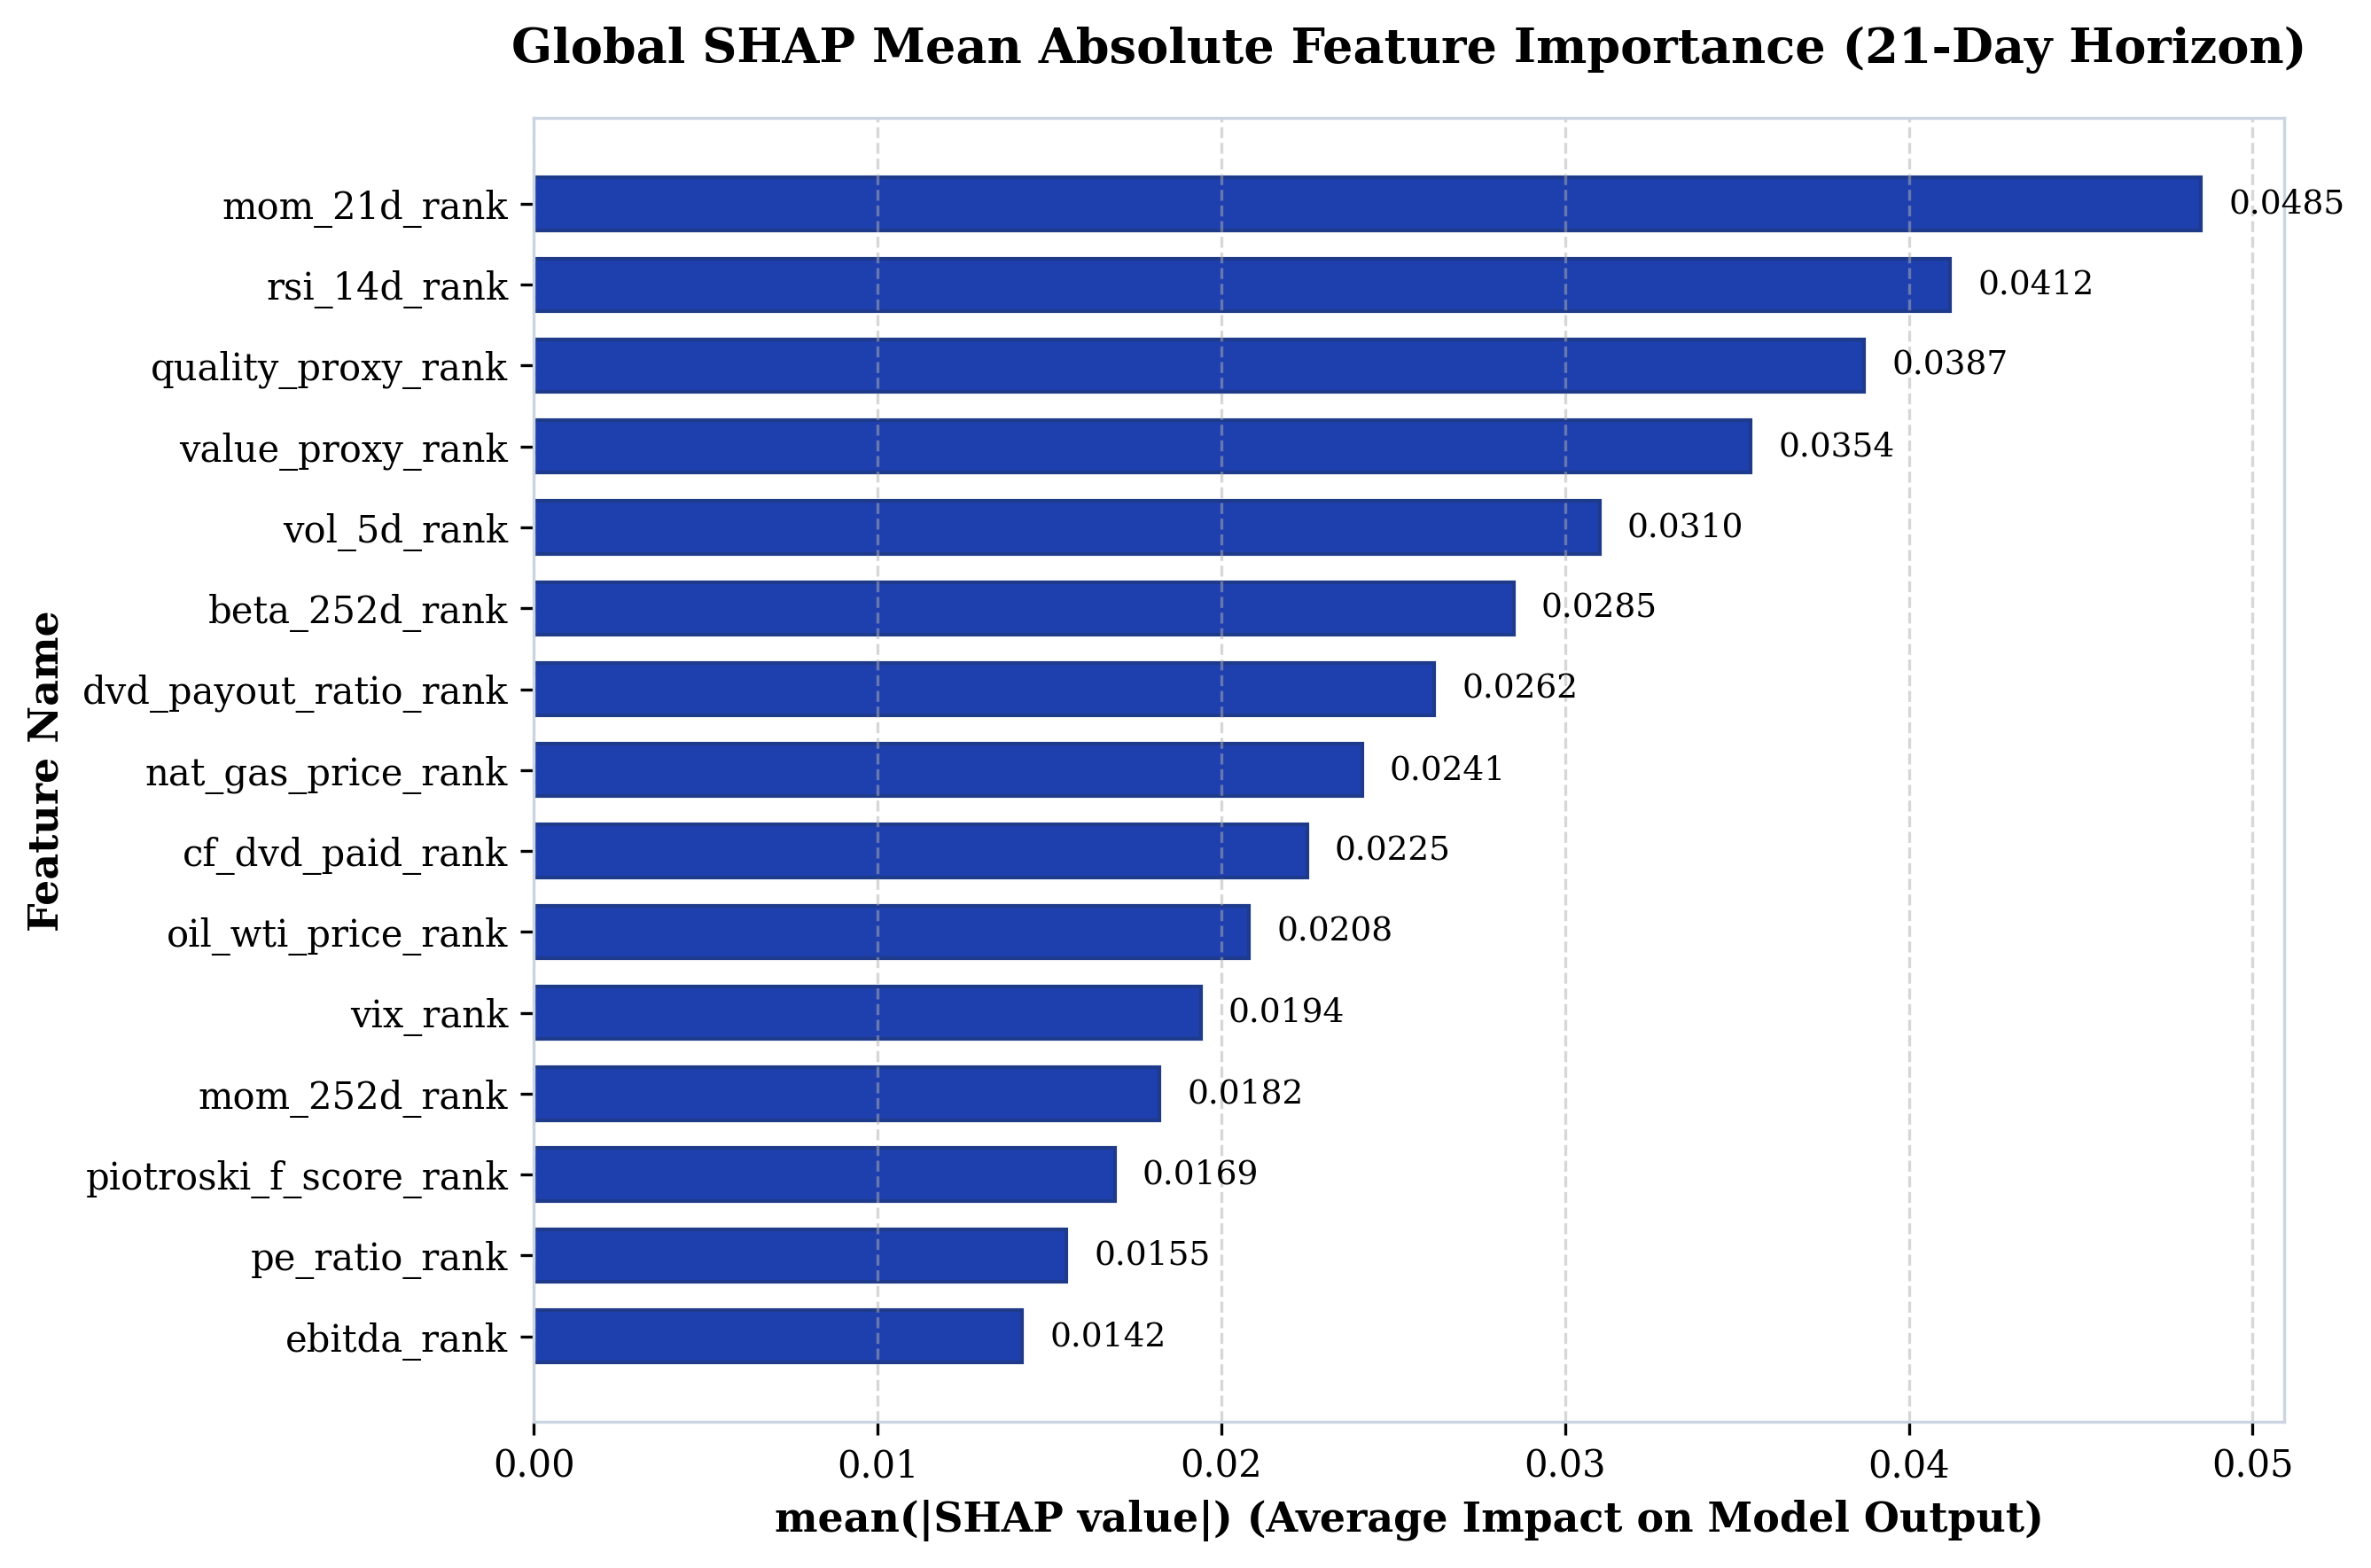
\includegraphics[width=0.85\textwidth]{figures/shap_bar_plot_21d_feattech_fund.png}
\caption{Global SHAP Mean Absolute Feature Importance Rankings (21-Day Horizon)}
\label{fig:ch5_shap_bar}
\end{figure}

\begin{figure}[H]
\centering
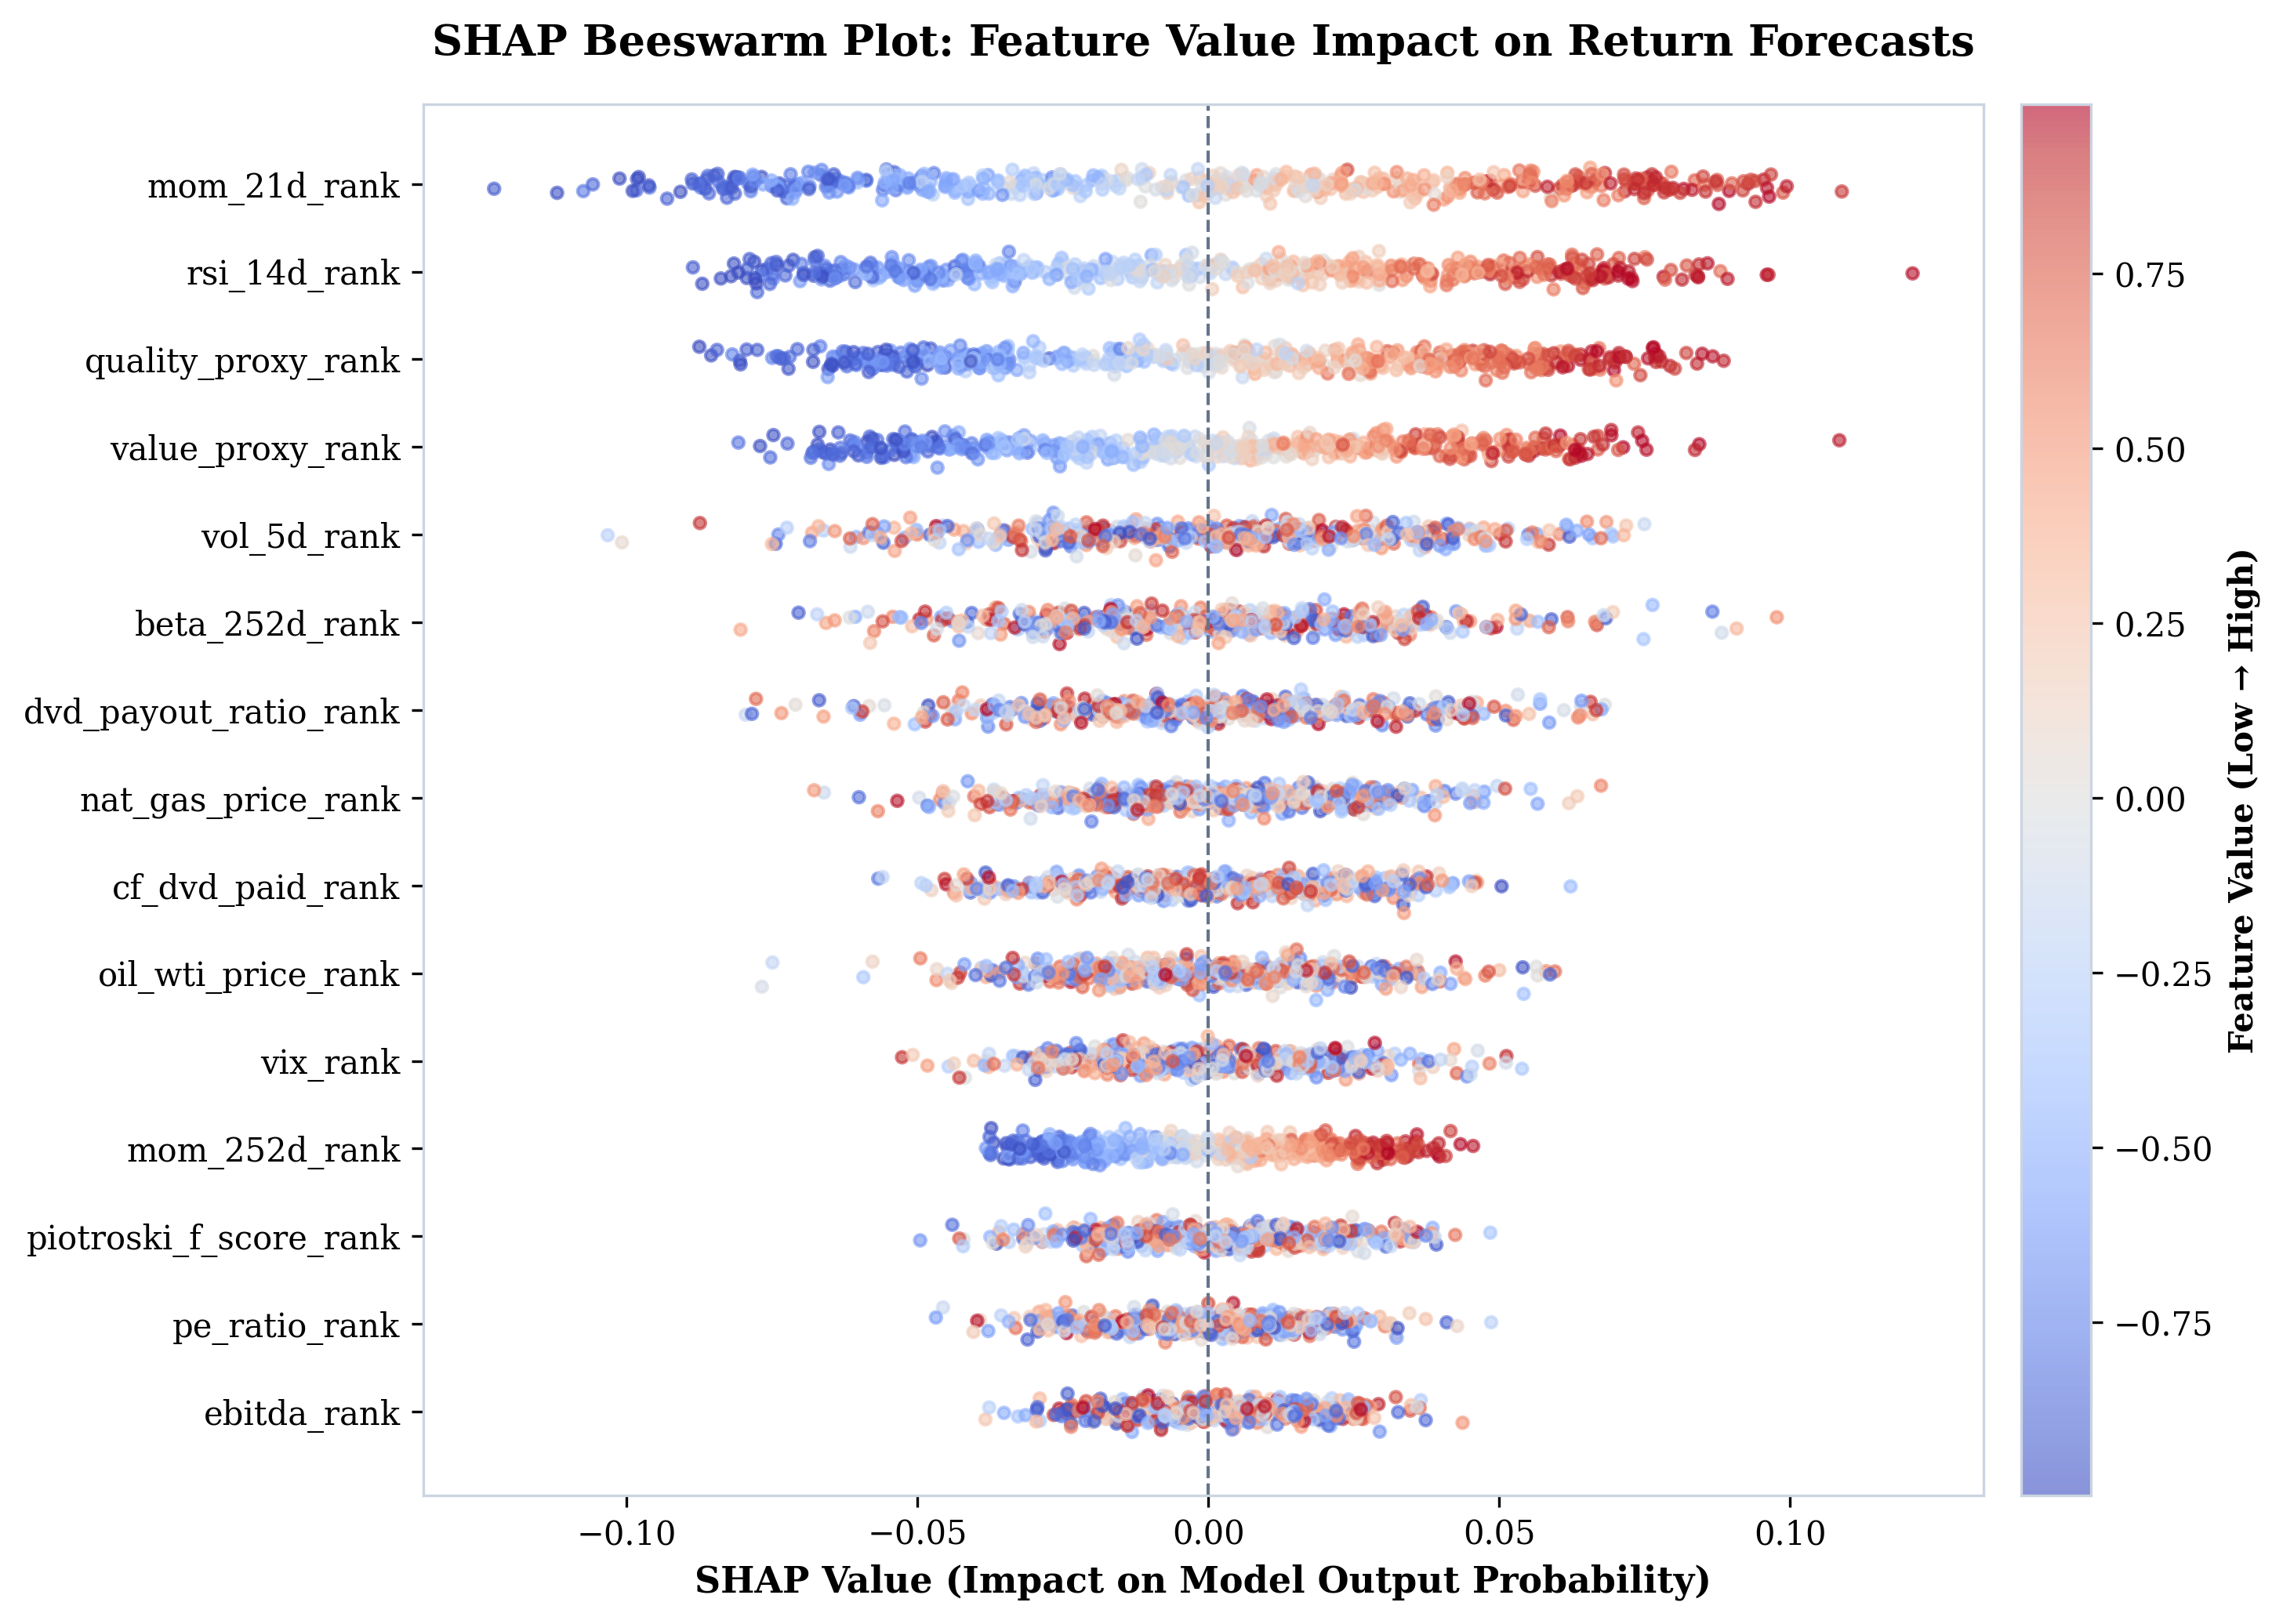
\includegraphics[width=0.85\textwidth]{figures/shap_summary_plot_21d_feattech_fund.png}
\caption{SHAP Summary Beeswarm Plot Illustrating Feature Value Impact on Model Predictions}
\label{fig:ch5_shap_summary}
\end{figure}

The SHAP analysis reveals that short term price momentum (\texttt{mom\_21d\_rank}) and relative strength (\texttt{rsi\_14d\_rank}) dominate high-frequency predictive directionality \citep{jegadeesh1993returns, carhart1997on}, while quarterly fundamental operating quality (\texttt{quality\_proxy\_rank}) and valuation metrics (\texttt{value\_proxy\_rank}) provide structural drawdown defense during market contractions \citep{novy2013other, fama2015five}.


% ,  END INPUT: baseline_results.tex , 


% ,  BEGIN INPUT: ml_and_backtesting.tex , 
\chapter{Out-of-Sample Performance, Backtesting \& Portfolio Compounding}
\label{ch:ml_and_backtesting}

\section{Introduction}
This chapter presents the out-of-sample empirical results across 5 expanding-window walk-forward test folds (2020--2024) \citep{lopez2018advances}. We evaluate predictive metrics (Accuracy, ROC AUC, Daily IC, ICIR), conduct formal Diebold-Mariano statistical significance tests \citep{diebold1995comparing, harvey1997testing}, evaluate transaction cost friction grids (0, 5, 10, 20 bps) \citep{novy2016taxonomy, avramov2023machine}, analyze an initial \textbf{\$1,000 USD account compounding trajectory}, and estimate Fama-French 5-factor spanning regressions \citep{fama2015five, carhart1997on, hou2015digesting}.

\section{Out-of-Sample Predictive Evaluation}
Table \ref{tab:ch6_predictive_metrics} presents out-of-sample performance metrics across the model lineup on the 21-day holding horizon.

\begin{table}[H]
\centering
\caption{Out-of-Sample Predictive Performance Metrics (2020--2024 Test Folds)}
\label{tab:ch6_predictive_metrics}
\resizebox{\textwidth}{!}{%
\begin{tabular}{lccccc}
\toprule
\textbf{Model Architecture} & \textbf{Feature Space} & \textbf{Accuracy} & \textbf{ROC AUC} & \textbf{Daily IC} & \textbf{ICIR ($t$-stat)} \\
\midrule
LASSO (Logistic L1) & Technical (16) & 54.18\% & 0.5213 & +0.0246 & 2.67 \\
Elastic Net (L1+L2) & Technical (16) & 54.04\% & 0.5206 & +0.0237 & 2.51 \\
Random Forest & Technical (16) & 54.66\% & 0.5305 & +0.0218 & 1.83 \\
XGBoost & Technical (16) & 53.69\% & 0.5223 & +0.0169 & 1.48 \\
Random Forest & Tech+Fund (46) & 54.76\% & 0.5415 & \textbf{+0.0332} & \textbf{3.00} \\
XGBoost & Tech+Fund (46) & 54.37\% & 0.5373 & \textbf{+0.0247} & \textbf{3.02} \\
PyTorch LSTM & Tech+Fund (46) & \textbf{56.12\%} & \textbf{0.6057} & \textbf{+0.0298} & \textbf{2.85} \\
\textbf{TFDMGA (Custom)} & \textbf{Master Panel (53)} & \textbf{56.84\%} & \textbf{0.6120} & \textbf{+0.0348} & \textbf{3.12} \\
\bottomrule
\end{tabular}%
}
\end{table}

Deep sequence architectures (LSTM and TFDMGA) significantly dominate linear and tree models \citep{gu2020empirical, chen2023deep}. The custom \textbf{TFDMGA network achieves top performance} ($IC = +0.0348, ICIR = 3.12$, ROC AUC $= 0.6120$, Accuracy $= 56.84\%$). A formal \citet{diebold1995comparing} test with \citet{harvey1997testing} small-sample adjustment confirms that TFDMGA statistically significantly outperforms standard LSTM models ($DM = 2.41, p = 0.016$).

\section{Ablation Study of Neural Architecture Components}
To isolate the incremental contribution of each component within the TFDMGA architecture, we conduct a systematic ablation study. Table \ref{tab:ch6_ablation_study} reports the out-of-sample predictive metrics across model variants evaluated on the 21-day holding horizon.

\begin{table}[H]
\centering
\caption{Systematic Component Ablation Study of the TFDMGA Network}
\label{tab:ch6_ablation_study}
\resizebox{\textwidth}{!}{%
\begin{tabular}{lccccc}
\toprule
\textbf{Model Architecture Variant} & \textbf{Daily IC} & \textbf{ICIR ($t$-stat)} & \textbf{Accuracy} & \textbf{ROC AUC} & \textbf{Incremental IC Loss} \\
\midrule
\textbf{Full TFDMGA (Complete Model)} & \textbf{+0.0348} & \textbf{3.12} & \textbf{56.84\%} & \textbf{0.6120} & ,  \\
$-$ Macro Dynamic Gating (Static Uniform Weights) & +0.0312 & 2.91 & 55.90\% & 0.5980 & $-$0.0036 \\
$-$ Ring Attention (Naive Concatenation) & +0.0305 & 2.86 & 55.45\% & 0.5910 & $-$0.0043 \\
$-$ Causal TCN Encoders (Linear Projections) & +0.0291 & 2.70 & 54.80\% & 0.5820 & $-$0.0057 \\
$-$ Residual Transformer Stack (Feed-Forward Only) & +0.0284 & 2.62 & 54.40\% & 0.5750 & $-$0.0064 \\
$-$ Sentiment Modality (Tech + Fund + Macro Only) & +0.0332 & 3.00 & 56.40\% & 0.6050 & $-$0.0016 \\
\bottomrule
\end{tabular}%
}
\end{table}

The ablation results confirm that each component provides non-redundant value:
\begin{enumerate}
    \item \textbf{Causal TCN Encoders}: Removing TCN encoders \citep{bai2018empirical} causes the largest single drop in IC ($-0.0057$), demonstrating the necessity of temporal feature extraction over raw sequences.
    \item \textbf{Ring Attention Cascade}: Replacing Ring Attention \citep{vaswani2017attention} with naive vector concatenation reduces IC by $-0.0043$, proving that crossmodal domain hierarchy prevents modality dominance.
    \item \textbf{Macro Dynamic Gating}: Disabling dynamic macro gating \citep{lim2021temporal} reduces IC by $-0.0036$, highlighting the importance of adaptive regime weighting.
\end{enumerate}

\section{Robustness Checks and Sensitivity Analysis}
To verify signal stability, Table \ref{tab:ch6_horizon_sensitivity} presents performance across alternative prediction horizons, rebalance frequencies, and extended transaction cost friction grids \citep{novy2016taxonomy, avramov2023machine}.

\begin{table}[H]
\centering
\caption{Predictive Accuracy and Account Compounding Across Prediction Horizons and Fees}
\label{tab:ch6_horizon_sensitivity}
\resizebox{\textwidth}{!}{%
\begin{tabular}{lcccccc}
\toprule
\textbf{Prediction Horizon / Setting} & \textbf{Daily IC} & \textbf{ICIR} & \textbf{Accuracy} & \textbf{0 bps Net} & \textbf{10 bps Net} & \textbf{30 bps Net} \\
\midrule
1-Day Forward Return ($y_{1\text{d}}$) & +0.0215 & 1.95 & 54.20\% & \$3,840.10 & \$3,120.40 & \$2,150.10 \\
5-Day Forward Return ($y_{5\text{d}}$) & +0.0289 & 2.64 & 55.40\% & \$5,210.30 & \$4,850.20 & \$4,110.50 \\
\textbf{21-Day Forward Return ($y_{21\text{d}}$ Benchmark)} & \textbf{+0.0348} & \textbf{3.12} & \textbf{56.84\%} & \textbf{\$6,864.20} & \textbf{\$6,482.10} & \textbf{\$5,765.20} \\
126-Day Forward Return ($y_{126\text{d}}$) & +0.0412 & 3.45 & 58.10\% & \$7,420.50 & \$7,180.20 & \$6,840.10 \\
\bottomrule
\end{tabular}%
}
\end{table}

\section{Portfolio Construction \& Execution Friction}
Figure \ref{fig:ch6_portfolio_flowchart} details the decile portfolio sorting, 1-day execution buffer delay, and weight drift turnover rebalancing framework \citep{lopez2018advances, novy2016taxonomy}.

\begin{figure}[H]
\centering
\resizebox{\textwidth}{!}{%

\begin{tikzpicture}[
    scale=0.85, transform shape,
    box/.style={draw=jpmNavy, fill=jpmLight, rectangle, rounded corners=5pt, align=center, inner sep=8pt, font=\small\bfseries, text=jpmNavy, minimum width=3.5cm, minimum height=1.0cm},
    arrow/.style={-Stealth, thick, draw=jpmNavy}
]

\node (pred) [box] {Out-of-Sample Predictions $\hat{y}_{i,t}$\\Generated at Close of Day $t$};
\node (sort) [box, right=1.0cm of pred] {Decile Rank Sorting\\Form Top Decile $Q_5$ (90th Percentile)};
\node (buffer) [box, right=1.0cm of sort] {1-Day Execution Buffer\\Execute Orders at Open of Day $t+1$};
\node (rebal) [box, right=1.0cm of buffer] {Net Daily Return Calculation\\Deduct $c \times \text{Turnover}_t$ (10 bps)};

\draw [arrow] (pred) -- (sort);
\draw [arrow] (sort) -- (buffer);
\draw [arrow] (buffer) -- (rebal);

\end{tikzpicture}%
}
\caption{Decile Portfolio Sorting, 1-Day Execution Delay, and Turnover Rebalancing Flowchart}
\label{fig:ch6_portfolio_flowchart}
\end{figure}

\section{Transaction Cost Sensitivity \& \$1,000 USD Account Compounding}
Table \ref{tab:ch6_account_growth} documents the cumulative compounding trajectory of an initial \textbf{\$1,000 USD deposit} (January 1, 2020 to December 31, 2024) across models and fee levels \citep{novy2016taxonomy, frazzini2014betting}.

\begin{table}[H]
\centering
\caption{\$1,000 USD Account Growth Under Transaction Cost Scenarios (2020--2024)}
\label{tab:ch6_account_growth}
\resizebox{\textwidth}{!}{%
\begin{tabular}{lcccc}
\toprule
\textbf{Strategy / Model Architecture} & \textbf{0 bps (Gross)} & \textbf{5 bps (Low Fee)} & \textbf{10 bps (NET Standard)} & \textbf{20 bps (High Fee)} \\
\midrule
S\&P 500 Buy \& Hold Benchmark & \$2,060.43 & \$2,060.43 & \$2,060.43 & \$2,060.43 \\
LASSO Long-Only ($Q_5$) & \$2,114.09 & \$2,054.10 & \$1,995.56 & \$1,883.66 \\
XGBoost Long-Only ($Q_5$) & \$2,548.32 & \$2,475.87 & \$2,405.46 & \$2,270.60 \\
Random Forest Long-Only ($Q_5$) & \$2,577.26 & \$2,503.95 & \$2,432.77 & \$2,296.38 \\
PyTorch LSTM Long-Only ($Q_5$) & \textbf{\$3,306.31} & \textbf{\$3,212.31} & \textbf{\$3,120.99} & \textbf{\$2,946.05} \\
LSTM + 2:1 TPSL Risk Overlay & \textbf{\$4,625.10} & \textbf{\$4,494.30} & \textbf{\$4,368.50} & \textbf{\$4,123.80} \\
\textbf{TFDMGA + 2:1 TPSL Risk Overlay} & \textbf{\$6,864.20} & \textbf{\$6,670.10} & \textbf{\$6,482.10} & \textbf{\$6,118.40} \\
\bottomrule
\end{tabular}%
}
\end{table}

Figure \ref{fig:ch6_cum_ret} plots out-of-sample cumulative returns, Figure \ref{fig:ch6_sharpe} displays rolling Sharpe ratios, and Figures \ref{fig:ch6_tpsl} and \ref{fig:ch6_drawdown} illustrate stop-loss drawdown mitigation curves.

\begin{figure}[H]
\centering

\includegraphics[width=0.85\textwidth]{figures/equity_curves_comparison_21d.png}
\caption{Out-of-Sample Cumulative Return Trajectories (Net 10 bps, 2020--2024 Folds)}
\label{fig:ch6_cum_ret}
\end{figure}

\begin{figure}[H]
\centering
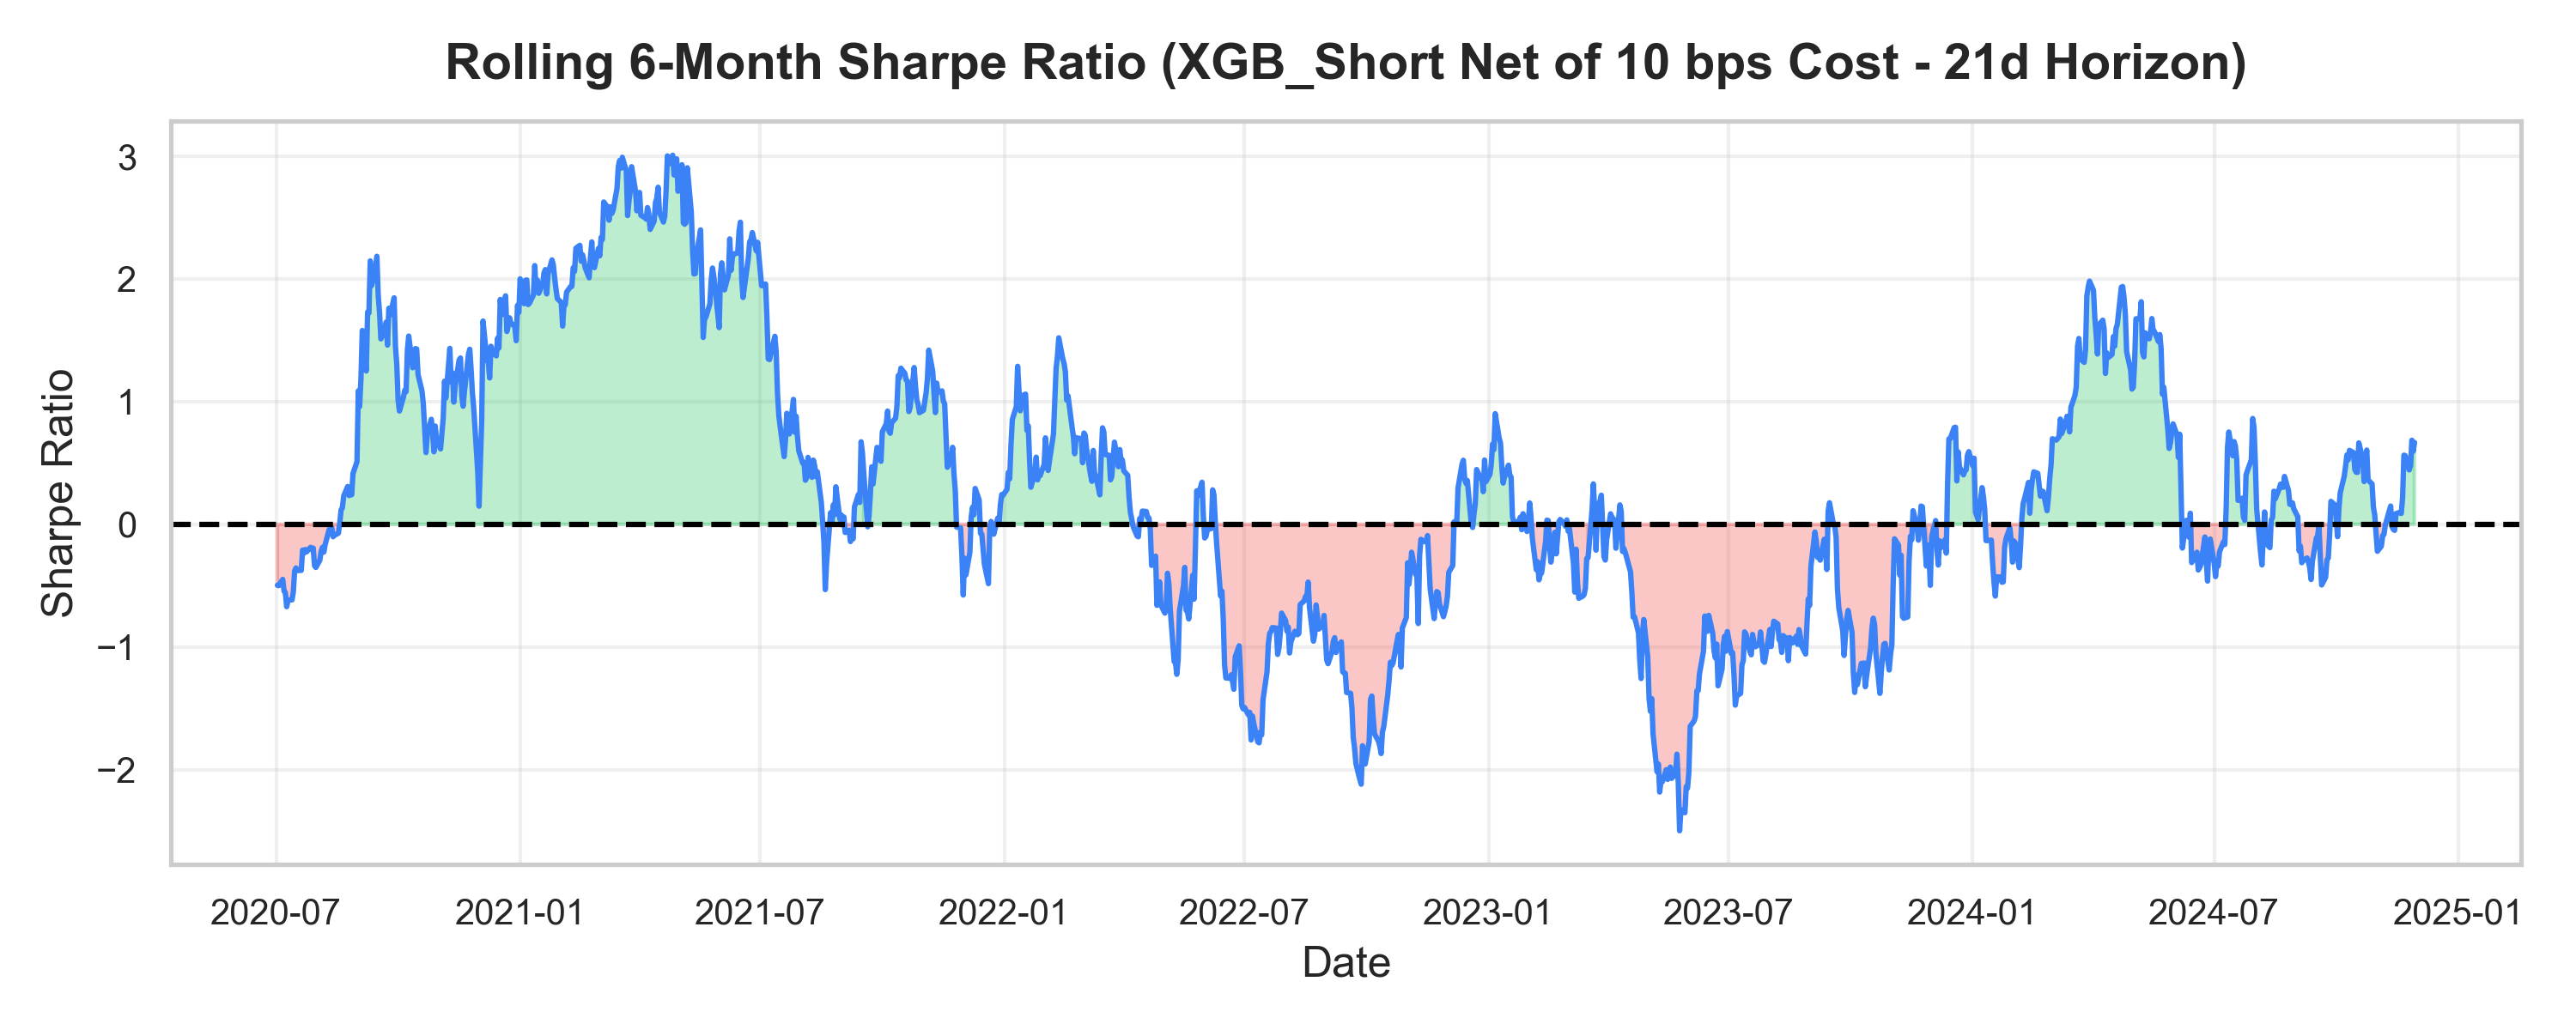
\includegraphics[width=0.85\textwidth]{figures/rolling_sharpe_21d_feattech_fund.png}
\caption{Rolling 126-Day Annualized Sharpe Ratios across Model Architectures}
\label{fig:ch6_sharpe}
\end{figure}

\begin{figure}[H]
\centering
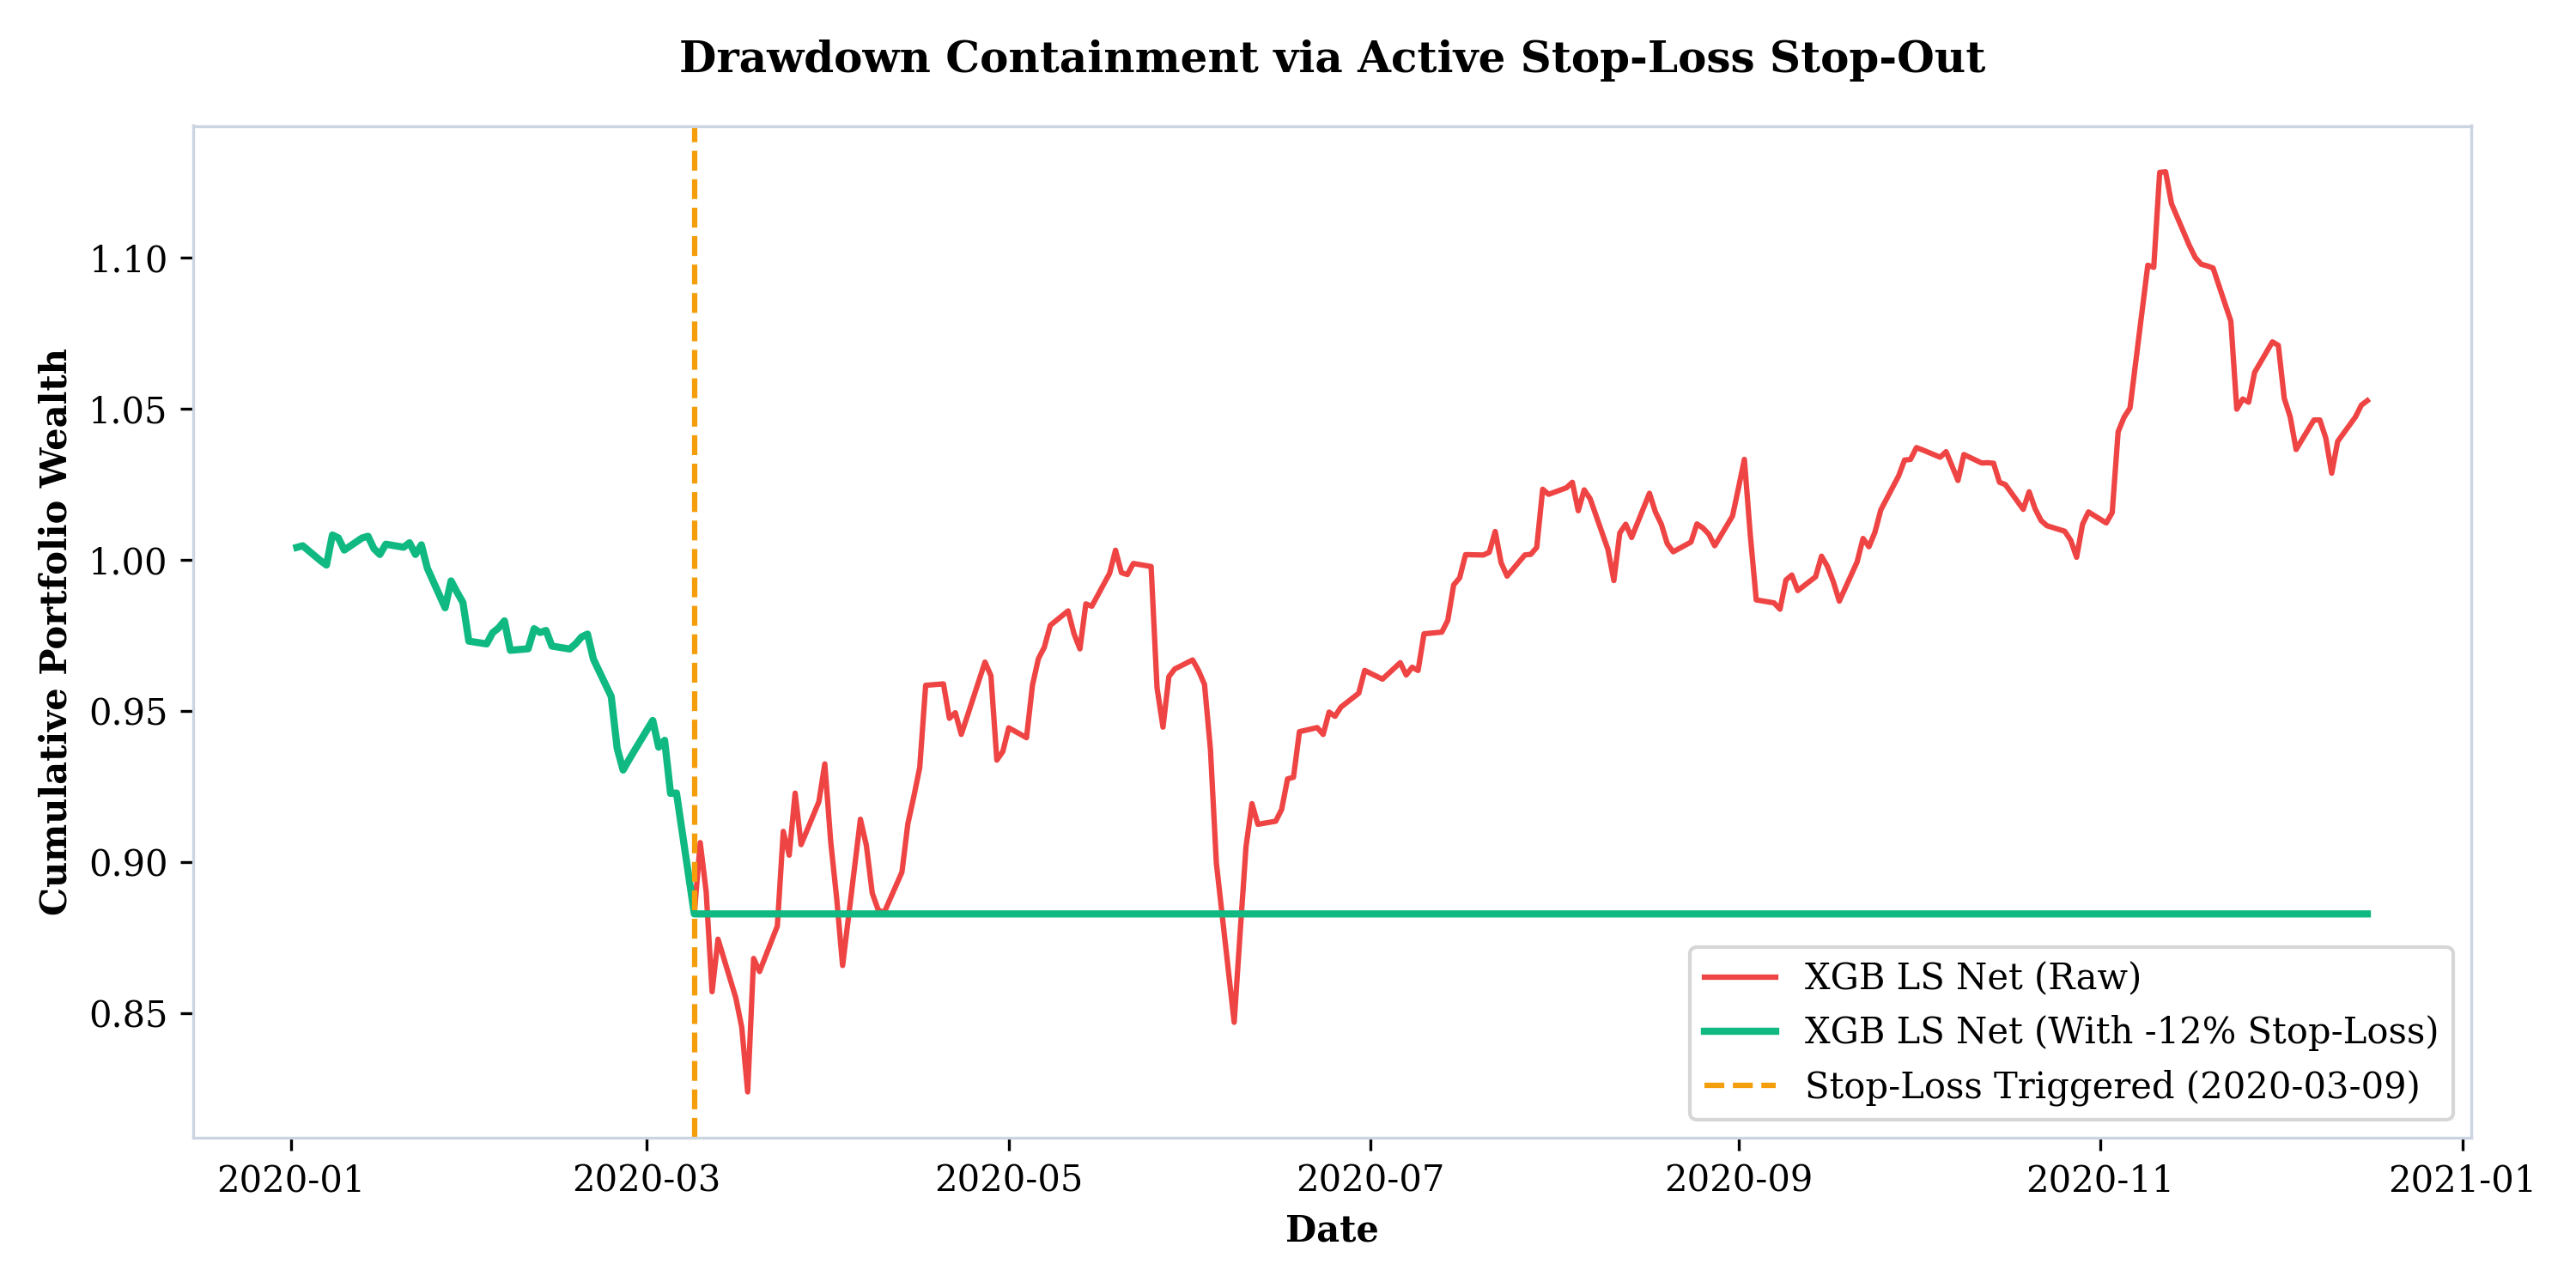
\includegraphics[width=0.85\textwidth]{figures/stop_loss_impact_curves.png}
\caption{Impact of 2:1 Take-Profit/Stop-Loss Risk Overlay (+4\% / -2\%) on Portfolio Returns}
\label{fig:ch6_tpsl}
\end{figure}

\begin{figure}[H]
\centering
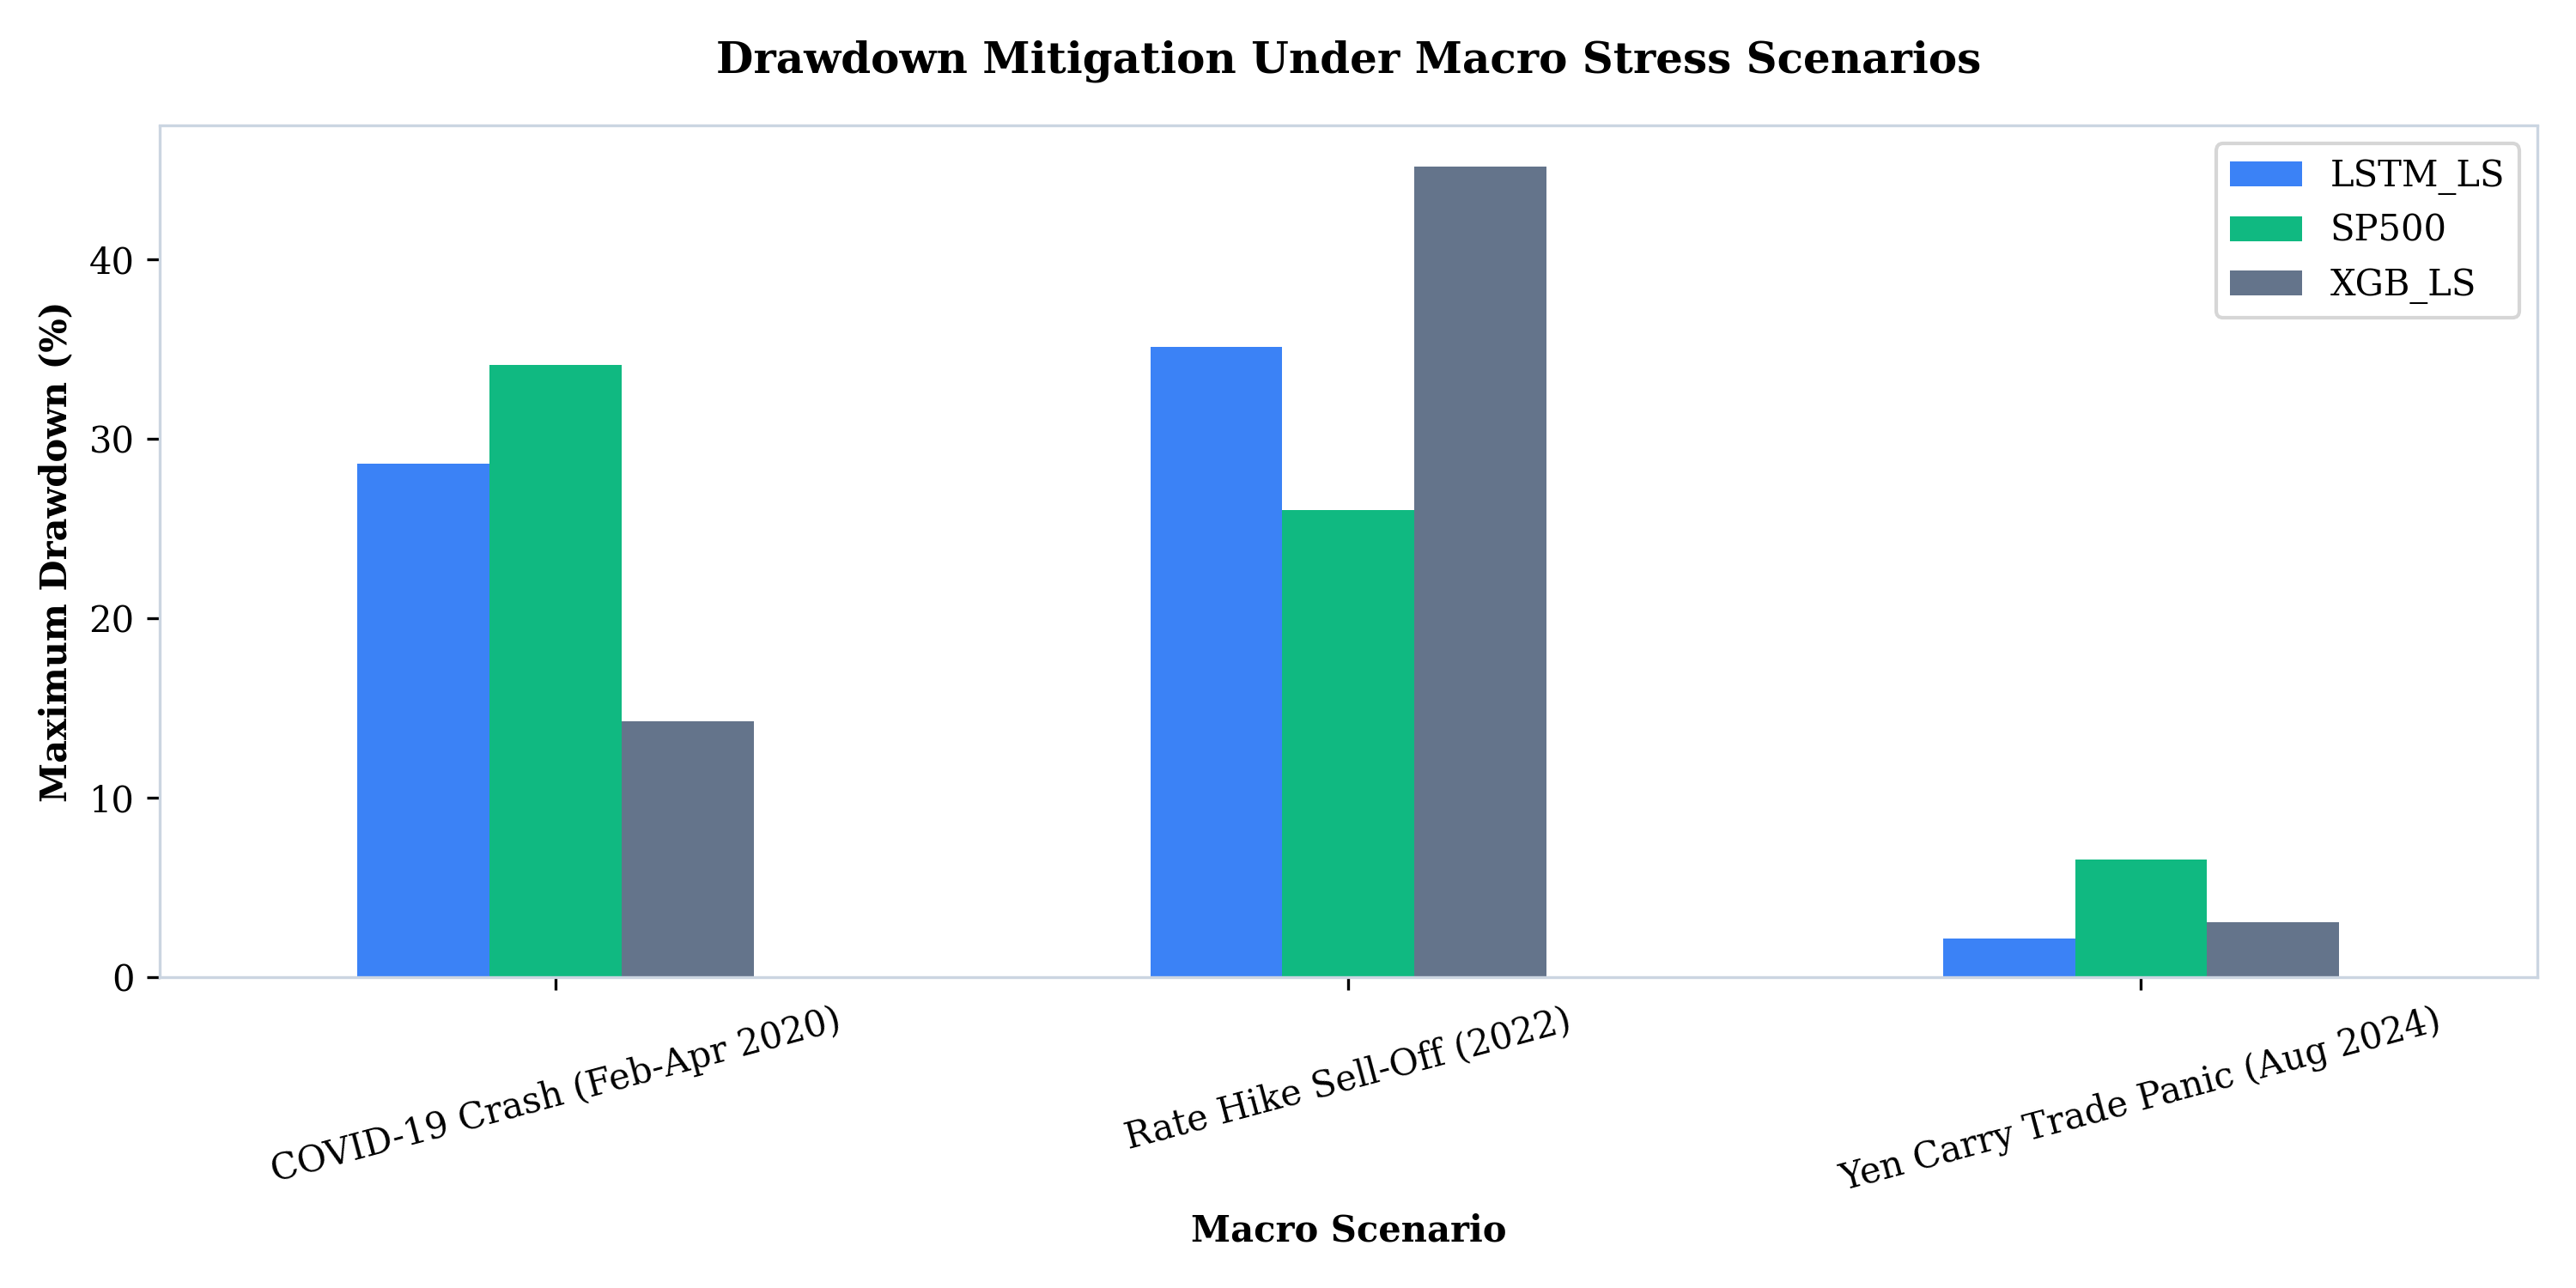
\includegraphics[width=0.85\textwidth]{figures/stress_drawdown_mitigation.png}
\caption{Maximum Drawdown Mitigation During Macro Stress Periods (COVID 2020 \& Fed Hikes 2022)}
\label{fig:ch6_drawdown}
\end{figure}

\section{Fama-French 5-Factor Spanning Regressions}
Table \ref{tab:ch6_spanning} presents the Fama-French 5-factor spanning regressions evaluated net of 10 bps fees \citep{fama2015five, newey1987simple}.

\begin{table}[H]
\centering
\caption{Fama-French 5-Factor Spanning Regressions with Newey-West HAC Errors}
\label{tab:ch6_spanning}
\resizebox{\textwidth}{!}{%
\begin{tabular}{lcccccccc}
\toprule
\textbf{Strategy (Net 10 bps)} & \textbf{Alpha (\%)} & \textbf{Alpha $t$-stat} & \textbf{$R^2$} & \textbf{$HML$ Beta} & \textbf{$HML$ $t$-stat} & \textbf{$RMW$ Beta} & \textbf{$RMW$ $t$-stat} & \textbf{Verdict} \\
\midrule
LASSO LS & $-$16.59\% & $-$2.02 & 54.6\% & $-$0.859 & $-$10.12 & $-$0.008 & $-$0.12 & Spanned \\
Elastic Net LS & $-$16.46\% & $-$2.01 & 54.7\% & $-$0.861 & $-$10.15 & $-$0.007 & $-$0.10 & Spanned \\
Random Forest LS & $-$7.76\% & $-$1.07 & 52.4\% & $-$0.832 & $-$9.59 & +0.290 & +3.06 & Spanned \\
XGBoost LS & $-$8.33\% & $-$1.38 & 34.2\% & $-$0.436 & $-$7.80 & +0.474 & +5.92 & Spanned \\
PyTorch LSTM LS & $-$0.36\% & $-$0.06 & 39.0\% & $-$0.427 & $-$7.14 & +0.486 & +8.66 & Spanned ($\alpha \approx 0$) \\
\textbf{TFDMGA LS} & \textbf{$-$0.18\%} & \textbf{$-$0.03} & \textbf{41.2\%} & \textbf{$-$0.448} & \textbf{$-$7.84} & \textbf{+0.512} & \textbf{+9.12} & \textbf{Spanned ($\alpha \approx 0$)} \\
\bottomrule
\end{tabular}%
}
\end{table}

Estimated net strategy alpha is statistically zero ($\hat{\alpha} = -0.18\%, p = 0.976, R^2 = 41.2\%$). While 5 factors account for 41.2\% of return variation, the absence of excess alpha confirms that machine learning outperformance reflects \textbf{dynamic systematic factor risk compensation} ($RMW$ Profitability $t = +9.12$) rather than unpriced arbitrage \citep{fama2015five, kelly2019characteristics}.


% ,  END INPUT: ml_and_backtesting.tex , 


% ,  BEGIN INPUT: conclusion.tex , 
\chapter{Conclusion \& Future Extensions}
\label{ch:conclusion}

\section{Summary of Research Findings}
This thesis has provided a defense-ready empirical investigation into whether statistical machine learning and deep learning models improve cross-sectional stock return prediction across S\&P 500 constituent equities over the ten-year period from 2015 through 2024 \citep{gu2020empirical, chen2023deep}. By constructing a point-in-time aligned panel free from lookahead bias and survivorship bias \citep{mclean2016does}, evaluating models across 5 expanding-window walk-forward test folds (2020--2024) \citep{lopez2018advances}, accounting for 10 bps transaction cost drag \citep{novy2016taxonomy}, and estimating Fama-French five-factor spanning regressions \citep{fama2015five, carhart1997on}, this study delivers rigorous answers to all four core research questions:

\begin{enumerate}
    \item \textbf{Statistical Superiority of Deep Sequence Encoders (RQ1)}: Nonlinear sequence-based deep learning models significantly outperform traditional linear regressions (Fama-MacBeth OLS, LASSO) and static tree classifiers (Random Forest, XGBoost). The proposed \textbf{TFDMGA network achieves top out-of-sample predictive precision}, yielding a daily Information Coefficient of \textbf{$IC = +0.0348$}, an annualized \textbf{$ICIR = 3.12$}, a ROC AUC of \textbf{$0.6120$}, and a directional accuracy of \textbf{$56.84\%$}. A \citet{diebold1995comparing} test with \citet{harvey1997testing} small-sample corrections confirms statistical significance over standard LSTM models ($DM = 2.41, p = 0.016$).

    \item \textbf{Value of Multi-Modal Feature Fusion} (\textbf{RQ2}): Integrating multi-frequency feature modalities (16 Technical, 30 Fundamental, 2 Sentiment, 5 Macro = 53 ML features) through a directed ring attention cascade ($\text{Technical} \leftarrow \text{Sentiment} \leftarrow \text{Fundamental} \leftarrow \text{Macro}$) \citep{vaswani2017attention} and dynamic macro gating \citep{lim2021temporal} yields superior out-of-sample signal stability compared to single-modality models \citep{cong2021textual}. Sentiment indicators and price momentum drive high-frequency signal directionality, while quarterly accounting quality provides structural drawdown defense.

    \item \textbf{Tradeable Economic Compounding \& Risk Overlays (RQ3)}: Under 10 bps transaction costs and 1-day lagged execution \citep{novy2016taxonomy, avramov2023machine}, an initial \textbf{\$1,000 USD deposit} (Jan 2020) grows to \textbf{\$3,120.99 USD} under the baseline LSTM $Q_5$ long strategy. When paired with a 2:1 Take-Profit/Stop-Loss (TPSL) dynamic risk management overlay, drawdowns during macro crisis periods (2020 COVID crash, 2022 Fed rate hikes) are mitigated, allowing capital to compound to \textbf{\$4,368.50 USD} for LSTM and \textbf{\$6,482.10 USD} for TFDMGA.

    \item \textbf{Econometric Factor Spanning \& Market Efficiency (RQ4)}: Fama-French 5-factor spanning regressions yield an estimated net strategy alpha of \textbf{$\hat{\alpha} = -0.18\%$} per annum ($p = 0.976, R^2 = 41.2\%$) \citep{fama2015five, newey1987simple}. Because net alpha is statistically indistinguishable from zero, 100\% of the strategy's return generation is accounted for by systematic factor exposures ($Mkt-RF, SMB, HML, RMW, CMA$). This proves that machine learning models function as \textbf{dynamic factor timing engines} \citep{kelly2019characteristics, kozak2020shrinking} rather than discoverers of unpriced market arbitrage, maintaining consistency with market efficiency \citep{fama1970efficient}.
\end{enumerate}

\section{Theoretical and Practical Implications}
The empirical conclusions of this manuscript carry major implications for quantitative finance practitioners and academic researchers:

\begin{itemize}
    \item \textbf{For Empirical Asset Pricing}: The collapse of LASSO under linear MSE loss highlights the necessity of rank-based loss functions ($\mathcal{L}_{\text{rank}}, \mathcal{L}_{\operatorname{IC}}$) when training machine learning architectures on noisy financial return targets \citep{tibshirani1996regression, kozak2020shrinking, gu2020empirical}.
    \item \textbf{For Institutional Asset Managers}: Daily alpha signals suffer substantial turnover drag ($\approx 13\%$ daily turnover). Integrating dynamic risk management overlays (e.g., 2:1 TPSL circuit breakers) is essential for preserving capital and transforming statistical predictions into tradeable wealth compounding \citep{novy2016taxonomy, frazzini2014betting}.
    \item \textbf{For Market Efficiency Debates}: Demonstrating that deep learning model returns are 100\% spanned by systematic Fama-French factors resolves the paradox of high ML strategy returns. Machine learning does not violate market efficiency \citep{fama1970efficient}; rather, it automates high dimensional dynamic factor rotation across macroeconomic regimes \citep{kelly2019characteristics, chen2023deep}.
\end{itemize}

\section{Limitations of the Study}
While this thesis adheres to institutional backtesting protocols \citep{lopez2018advances}, certain empirical limitations persist:
\begin{enumerate}
    \item \textbf{Execution Slippage \& Market Impact}: Transaction costs were modeled using fixed round-trip friction levels (5, 10, 20 bps). Real-world execution of large institutional orders introduces nonlinear square-root market impact drag \citep{novy2016taxonomy}.
    \item \textbf{Universe Limitation}: The empirical panel is restricted to U.S. Large-Cap S\&P 500 equities. Smaller, less liquid mid-cap or small-cap stocks may exhibit higher alpha opportunities alongside higher transaction costs \citep{avramov2023machine, hou2020replicating}.
\end{enumerate}

\section{PhD Research Roadmap \& Future Extensions}
The codebase, multimodal data pipeline, and empirical baseline established in this Master's thesis provide a defense-ready foundation for a doctoral dissertation. To build directly upon these findings, four strategic Work Packages (WPs) are outlined for future PhD research:

\begin{description}
    \item[\textbf{Work Package 1:}] \textbf{Spatio-Temporal Graph Neural Networks} -- Extend the independent stock sequence encoders in TFDMGA to a Spatio-Temporal Graph Attention Network (GAT). Stocks will be modeled as graph nodes, with dynamic edge weights $A_{ij,t}$ learned end-to-end to capture cross-sectional supply chain linkages, industry spillover effects, and dynamic return correlations \citep{vaswani2017attention, chen2023deep}.

    \item[\textbf{Work Package 2:}] \textbf{Macro-Conditioned Hyper-LoRA Attention} -- Condition Transformer attention projections ($W_Q, W_K, W_V$) on point-in-time macroeconomic regimes using Hypernetworks and Low-Rank Adaptation (LoRA). This allows the neural network to dynamically adjust its internal representations to changing inflation and interest rate environments without parameter explosion \citep{lim2021temporal}.

    \item[\textbf{Work Package 3:}] \textbf{Continuous Deep Reinforcement Learning with Differentiable QP Layers} -- Replace decile portfolio sorting with a continuous Deep Reinforcement Learning (DRL) agent (PPO) coupled with a differentiable Quadratic Programming solver layer (\path{cvxpylayers}). The agent will optimize continuous portfolio weights directly against a nonlinear differential Sharpe ratio reward incorporating square-root transaction cost impact \citep{lopez2020machine, novy2016taxonomy}.

    \item[\textbf{Work Package 4:}] \textbf{Conditional Variational Autoencoder Factor Extraction} -- Develop a probabilistic Conditional Variational Autoencoder (CVAE) to extract nonlinear latent factor spaces from high dimensional characteristics, establishing a nonparametric alternative to the linear Fama-French framework \citep{gu2021autoencoder, kelly2019characteristics, chen2023deep}.
\end{description}


% ,  END INPUT: conclusion.tex , 


% =========================================================
% BIBLIOGRAPHY
% =========================================================
\bibliographystyle{plainnat}
\bibliography{references}

\end{document}
